%%%%%%%%%%%%%%%%%%%%%%%%%%%%%%%%%%%%%%%%%
% Masters/Doctoral Thesis 
% LaTeX Template
% Version 1.41 (9/9/13), modified by David Rector
%
% This template was originally downloaded from:
% http://www.latextemplates.com
% before modification.
% 
% Original authors:
% Steven Gunn 
% http://users.ecs.soton.ac.uk/srg/softwaretools/document/templates/
% and
% Sunil Patel
% http://www.sunilpatel.co.uk/thesis-template/
%
% License:
% CC BY-NC-SA 3.0 (http://creativecommons.org/licenses/by-nc-sa/3.0/)
%
% 
%
%%%%%%%%%%%%%%%%%%%%%%%%%%%%%%%%%%%%%%%%%

%----------------------------------------------------------------------------------------
%       PACKAGES AND OTHER DOCUMENT CONFIGURATIONS
%----------------------------------------------------------------------------------------

\documentclass[12pt, a4paper, oneside]{Thesis} % Paper size, default font size and one-sided paper

\graphicspath{{Figures/}} % Specifies the directory where pictures are stored
\usepackage{enumerate}% http://ctan.org/pkg/enumerate
\usepackage[square, numbers, comma, sort&compress]{natbib} % Use the natbib reference package - read up on this to edit the reference style; if you want text (e.g. Smith et al., 2012) for the in-text references (instead of numbers), remove 'numbers' 
\usepackage{listings}
\usepackage{times}
\ifpaper
	\hypersetup{urlcolor=black, colorlinks=false, pdfborder={0 0 0}} % Makes links black, for better printing.
\else
	\hypersetup{urlcolor=blue, colorlinks=true} % Makes hyperlinks blue
\fi
	

\title{\ttitle} % Defines the thesis title - don't touch this

\usepackage{setspace}
\usepackage{lipsum}% just to generate filler text

\iffinal
	% Do nothing
\else
	% DWR: watermark package
	%\usepackage{draftwatermark} %use this and not next line if you want watermark on every page
	\usepackage[firstpage]{draftwatermark} % if watermark only desired on first page
\fi



\begin{document}

%DWR: Draft watermark
\iffinal
	\clearpage
	% Do nothing here
\else
	\SetWatermarkText{DRAFT}
	\SetWatermarkLightness{0.9}
	\SetWatermarkScale{2}
\fi

\frontmatter % Use roman page numbering style (i, ii, iii, iv...) for the pre-content pages

%\setstretch{1.1} % Line spacing of 1.3



% Define the page headers using the FancyHdr package and set up for one-sided printing
\fancyhead{} % Clears all page headers and footers
%\rhead{\thepage} % Sets the right side header to show the page number
\lhead{} % Clears the left side page header

\pagestyle{fancy} % Finally, use the "fancy" page style to implement the FancyHdr headers

\newcommand{\HRule}{\rule{\linewidth}{0.5mm}} % New command to make the lines in the title page

% PDF meta-data
\hypersetup{pdftitle={\ttitle}}
\hypersetup{pdfsubject=\subjectname}
\hypersetup{pdfauthor=\authornames}
\hypersetup{pdfkeywords=\keywordnames}


% TITLE PAGE (to edit format, see titlePage.tex; to edit names/values, see docVars.tex)

%----------------------------------------------------------------------------------------
%       TITLE PAGE
%----------------------------------------------------------------------------------------

\begin{titlepage}
\begin{center}

\HRule \\[0.5cm] % Horizontal line

{\large \bfseries \ttitle} % Thesis title
\HRule % Horizontal line
\linespread{1.1} \\~\\[0.2cm]
  \textit{A Thesis Submitted to the Faculty\\in partial fulfillment of the requirements for the\\ degree of\\ \degreename}\\[0.2cm] % University requirement text
\textit{in}\\[0.3cm]
\fieldname\\[0.3cm] % Research group name and department name
 
%\begin{minipage}{0.4\textwidth}
%\begin{flushleft} \large
\large\emph{by}\\\Large
\textsc{\authornames}\\ % Author name - remove the \href bracket to remove the link
%\end{flushleft}
%\end{minipage}
 \textsc{\large \univname}\\ % University name
 \normalsize \citystatenames\\
 { \today}\\[2.0 cm] % Date
%\textsc{\Large Master's Thesis}\\[0.5cm] % Thesis type


\begin{minipage}{1.0\textwidth}
\begin{flushright} \large
\normalsize \emph{Examining Committee:} \\~\\
\underline{\hspace{6cm}}\\\small (chair) \textsc{\commchairname} \\~\\~ \underline{\hspace{6cm}}\\ \small\textsc{\commadvtwoname} \\~\\~ \underline{\hspace{6cm}}\\ \small\textsc{\commadvthreename}  
% to add a fourth advisor, follow format above, then adjust spacing, e.g. space after date, so that it fits on one paeg
\end{flushright}
\end{minipage}\\[1cm]

\begin{minipage}{1.0\textwidth}
\begin{flushleft} \large
\underline{\hspace{6cm}}\\ \small\textsc{\deangradstudiesname}\\
Dean of Graduate Studies
\end{flushleft}
\end{minipage}
 
 
\vfill
\end{center}

\end{titlepage}
\clearpage
\newpage\null\thispagestyle{empty}\newpage

%----------------------------------------------------------------------------------------
%       ABSTRACT PAGE
%----------------------------------------------------------------------------------------

\singlespacing
\clearpage
\thispagestyle{plain}
\pagestyle{plain}
\pagenumbering{roman}
\setcounter{page}{2}

\addtotoc{Abstract} % Add the "Abstract" page entry to the Contents

\abstract{\addtocontents{toc}{\vspace{1em}} % Add a gap in the Contents, for aesthetics
\thispagestyle{plain}
\pagestyle{plain}
\pagenumbering{roman}
\setcounter{page}{2}
\abstracttextfull
}

\clearpage % Start a new page



%----------------------------------------------------------------------------------------
%       QUOTATION PAGE
%----------------------------------------------------------------------------------------

%\pagestyle{empty} % No headers or footers for the following pages

\null\vfill % Add some space to move the quote down the page a bit
\null\vfill

\textit{\quotetextfull}

\begin{flushright}
\quoteattrname
\end{flushright}

\vfill\vfill\vfill\vfill\vfill\vfill\null % Add some space at the bottom to position the quote just right

\clearpage % Start a new page


%----------------------------------------------------------------------------------------
%       ACKNOWLEDGMENTS
%----------------------------------------------------------------------------------------

\setstretch{1.3} % Reset the line-spacing to 1.3 for body text (if it has changed)

\acknowledgments{\addtocontents{toc}{\vspace{1em}} % Add a gap in the Contents, for aesthetics
\acknowtextfull
}
\clearpage % Start a new page

%----------------------------------------------------------------------------------------
%       LIST OF CONTENTS/FIGURES/TABLES PAGES
%----------------------------------------------------------------------------------------

\pagestyle{fancy} % The page style headers have been "empty" all this time, now use the "fancy" headers as defined before to bring them back

\lhead{\emph{Contents}} % Set the left side page header to "Contents"
\hypertarget{contents}{}
\tableofcontents % Write out the Table of Contents

\lhead{\emph{List of Figures}} % Set the left side page header to "List of Figures"
\listoffigures % Write out the List of Figures

%\lhead{\emph{List of Tables}} % Set the left side page header to "List of Tables"
%\listoftables % Write out the List of Tables

%----------------------------------------------------------------------------------------
%       ABBREVIATIONS
%----------------------------------------------------------------------------------------

%\clearpage % Start a new page

%\setstretch{1.5} % Set the line spacing to 1.5, this makes the following tables easier to read

%\lhead{\emph{Abbreviations}} % Set the left side page header to "Abbreviations"
%\listofsymbols{ll} % Include a list of Abbreviations (a table of two columns)
%{
%\textbf{LAH} & \textbf{L}ist \textbf{A}bbreviations \textbf{H}ere \\
%\textbf{Acronym} & \textbf{W}hat (it) \textbf{S}tands \textbf{F}or \\
%}

%----------------------------------------------------------------------------------------
%       PHYSICAL CONSTANTS/OTHER DEFINITIONS
%----------------------------------------------------------------------------------------

%\clearpage % Start a new page

%\lhead{\emph{Physical Constants}} % Set the left side page header to "Physical Constants"

%\listofconstants{lrcl} % Include a list of Physical Constants (a four column table)
%{
%Speed of Light & $c$ & $=$ & $2.997\ 924\ 58\times10^{8}\ \mbox{ms}^{-\mbox{s}}$ (exact)\\
% Constant Name & Symbol & = & Constant Value (with units) \\
%}

%----------------------------------------------------------------------------------------
%       SYMBOLS
%----------------------------------------------------------------------------------------

%\clearpage % Start a new page

%\lhead{\emph{Symbols}} % Set the left side page header to "Symbols"

%\listofnomenclature{lll} % Include a list of Symbols (a three column table)
%{
%$a$ & distance & m \\
%$P$ & power & W (Js$^{-1}$) \\
% Symbol & Name & Unit \\

%& & \\ % Gap to separate the Roman symbols from the Greek

%$\omega$ & angular frequency & rads$^{-1}$ \\
% Symbol & Name & Unit \\
%}

%----------------------------------------------------------------------------------------
%       DEDICATION
%----------------------------------------------------------------------------------------

\setstretch{1.1} % Return the line spacing back to 1.3

\pagestyle{empty} % Page style needs to be empty for this page

\dedicatory{\large{\dedicationtext}} % Dedication text

\addtocontents{toc}{\vspace{2em}} % Add a gap in the Contents, for aesthetics

%----------------------------------------------------------------------------------------
%       THESIS CONTENT - CHAPTERS & APPENDICES
%----------------------------------------------------------------------------------------

\doublespacing % if you want a copy that is single spaced, use \singlespacing.  If you want 1.5 spacing, use \onehalfspacing
\mainmatter % Begin numeric (1,2,3...) page numbering
\pagestyle{fancy} % Return the page headers back to the "fancy" style

%----------------------------------------------------------------------------------------
%       THESIS CONTENT - CHAPTERS
%----------------------------------------------------------------------------------------

% ----------------------------------------------------------------------------------------
% INTRODUCTION
% ----------------------------------------------------------------------------------------
\chapter{Introduction}\label{introduction}
\lhead{\chaptertitlename\ \thechapter. \emph{Introduction}}
% ----------------------------------------------------------------------------------------



\section{a custom aesthetic}

Music and electronics are ``comfortably interrelated'' \citep{kettelkamp1984}. The space within which electronics are conceptualized and developed is defined by the technical means available to the designer and manufacturer. Advances in hardware specifications allow for increasingly sophisticated implementation of analog and digital signal processing techniques, as well as more robust, elegant or inspiring human/machine interfaces.  
	
Audio devices, as a subset of consumer electronics, are bound by those technical limitations. Both corresponding markets see product updates every time a significant subset of those limitations evolve. Beyond those common boundaries, however, audio electronics design and a generalist engineering practice exhibit different approaches to innovation and renewal. 

In the 1960's, transistors rendered the dangerous and inefficient vacuum tube obsolete in most devices except for very high frequency circuits and audio amplifiers \citep{barbour1998}. The latter case is an early example of inefficient systems being maintained for aesthetic considerations: vacuum tubes produced specific nonlinearities, internalized as a cultural bias that has perpetuated the relevance of an otherwise antiquated technology \citep{barbour1998}. That favoritism is based in subjectivity - some music practitioners prefer solid state amplifiers for an arbitrary subset of qualities the technology offers \citep{hamm1973}. Different musical backgrounds and experiences inform the technical choices made in the design of each musician's specific setup. Specifically, they influence which limitations, materialized as imperfections, are acceptable in a personal musical system. Vacuum tubes are only one instance of this phenomena amongst many: discrete transistors, analog synthesizers, low-resolution digital audio, etc.  

The task of designing electronic music instruments can not be reduced to a set of performance requirements for a circuit, algorithms, or both. Viewing instruments as optimal machines does not do justice to their potential as catalysts of poetic experiences - interesting results arise when designers explicitly address them as post-optimal objects \citep{dunne2005}. Successful instruments must inspire their users, helping them to transform abstractions and intuitions into a concrete sonic output, with limitations often proving inspirational \citep{evens2005,rovan2009}. Don Buchla, in designing his \"music boxes\", describes himself as a builder of instruments rather than of machines. He is intentionally addressing a limited market of small commercial potential \citep{pinch2001}. Nic Collins brings this one step further by coining the term silicon luthier, the craftsperson of electronic music \citep{collins2008}. By intentionally limiting a user base, Buchla and Collins both suggest that electronic music instruments can benefit from a small-scale, custom approach in both the design and manufacturing processes. 

This benefit is compounded by the constantly evolving nature of electronic hardware and the digital software it often hosts. Technological advances are not correlated to changes in aesthetics of music: compelling uses of a new instrument are as important as the design of the instrument itself \citep{braun2000}. Designing an instrument for a specific person or use increases its chances of successfully empowering a creative process. Addressing the issues inherent to ubiquitous performance and composition systems today is more efficiently done on a case-by-case basis \citep{armstrong2006,haslett2005}. 

That personal, inspiringly imperfect vision of electronic music instrument design materialized in various forms through the 20th century: invention, do-it-yourself (diy), hacking, circuit bending. Today, this set of historical practices joins back with trends in general hardware design, with movements such as the open source and maker movements ~\citep{mellis2014,perner2011}. Practitioners meet in FabLabs, which replace the garage and basements of previous generations ~\citep{mellis2011}. Both appear as symptomatic of a similar interest across user-bases: a desire take advantage of emerging technologies to create personal, more inspiring experiences for themselves and their audiences ~\citep{hermans2014}. The primary goal of this thesis is to contextualize and analyze the work of designers who fit within this vision of audio hardware, aware of precedents but challenging tradition and expectations through inspiring if imperfect uses of electronics.

\section{Motivation}

This work exists because of a deep curiosity for the instruments that makes a music electronic, their creators, and their place in today's art world. It hopes to foster future interdisciplinary research in the field of electronic music hardware and encourage open, experimental devices that blur the line between composition and design. 

Diy music instrument communities are based on sharing designs, advice and results. Successful resources document projects from start to end, with more than enough information to tackle any eventual mistake. These attributes find clear parallels in open source hardware design practices, as defined by the open source hardware association (OSHWA, w2015). By documenting and contextualizing relevant projects, one can contribute back to both communities. Furthermore, presenting this material in an academic context helps link these practitioners to some of the driving forces behind those emerging technologies. Some of the devices that have encouraged those communities still require strong corporate or academic backing (Arduino, Raspberry Pi). 

This ethnography of design practices in musical technologies should also illustrate an aspect of the interdisciplinary nature of music technology, allowing further comparisons and connections with other designers, trends and fields. By rooting contemporary electronic music practice to the hardware that enables it, a stronger bond to the developing field of sound art is favored ~\citep{cluett2013}. A more explicit connection is drawn to the people who make audio electronics, whether they are boutique designers or factory workers ~\citep{rylan2015}.  Issues arising from a direct transferal of design practices from an engineering based in market economies and cult of performance can be better identified, addressed, and solved for the further development of inspiring interfaces ~\citep{ghazala2004,christensen2005,Feldman2007,silver2009,perner2011,hertz2012,riis2013,jackson2014}.

\section{Scope and structure}

This work wishes to contextualize and analyze a selection of audio electronic systems as products of a technological, cultural and social environment. By acknowledging the products, prototypes, tools, and people involved in this process, a more accurate description of these ecosystems of invention can be achieved \citep{vinck2003}. This, in turn, allows for a clearer view of the possibilities and futures for the field of devices for musical expression. 
	
	For this clear description to emerge, this document will introduce a selective history of formative practices paralleling the history of modern electronics \citep{holmes2002}. Starting with the isolated forefathers of the field and their \"spirit of invention" \citep{dunn2001}, useful references through to Nic Collins' Handmade Electronic Music \citep{collins2006} will allow us to discuss the concepts of component design, system design and interaction design in a musical context. In this discussion, do-it-yourself, hacking and circuit bending are important, both in terms of general design and in how they apply to musical practices. We will then present the current incarnation of this spirit of invention and experimentation, in the greater context of making and musical cultures. This will be done through an analysis of specific projects from the last five to ten years and of interviews with their authors. As we'll see, open innovation \citep{christensen2005} and more specifically open hardware made and make electronic instrument design an ecosystem of invention. This ecosystem is thriving. 

	Linking this back to the field of experimental music, the paper concludes with a set of experiments based on those analyses of existing projects and provides documentation for those who might wish to develop ideas presented here.

\section{Retrospective}

Hacking is pervasive \citep{paradiso2008}. Open source hardware practices, which share a deep link to hardware hacking \citep{williams2012}, are the bridge between longstanding methods in electronic music instrument designs and innovations in the field of accessible invention and fabrication. Through the work undertaken in this project and the writing that came out of it, it was most important to convey that making instruments could be as deeply personal and creative as composition, with endless inspiring parallels, an activity no longer reserved to academics or professionals. The goal isn't to create perfect products, rather, it is to produce something you are happy to use for musical purposes, regardless of its hypothetical shortcomings. In an age where the White House organizes its on maker faire and half of the documented projects are artistic (White House, w2014), this work will not be alone.
	



% Note that you don't necessarily need to use parts; you can just list chapters in order.  But it is easy to separate into parts.

\clearpage % be sure to have clearpage before each new part, so links work right.  If not using parts, not necessary.
\part{Past: the infancy of musical electronics}  %Whenever you want a new part, just put it in like this; part page & toc will auto-generate
% ----------------------------------------------------------------------------------------
% CHAPTER TITLE
% ----------------------------------------------------------------------------------------
\chapter{Experimental electronic systems in the musical arts: design concepts and history}\label{background}
\lhead{\chaptertitlename\ \thechapter. \emph{Background}}
% ----------------------------------------------------------------------------------------
\begin{quote}
	
	...not as descriptive of an act to be later judged in terms of success and failure, but simply as of an act the outcome of which is unknown. 
	
	\cite[p.13]{cage1961}
	
	\end{quote}
	
If experimental music is an act of uncertain consequences, transferring the concept over to engineering appears as counterintuitive. Great effort goes into making commercial electronics consistent, predictable and uniform. The same largely holds for electronic instruments - ``one-offs" with unpredictable behaviors or cryptic functions drastically reduce the overall adoption of the device, and therefore, their commercial potential \cite[p.5]{haslett2005}. In this context, the gap between the determinism of product design and the desire for originality of musical performances is bridged by the musician. ``Finding your sound" is about finding an instrument and using it effectively.  

Making, modifying or otherwise altering electronics is one option to better understand the tools at their disposal and make the most of them. Numerous historical precedents for personalized instruments will be presented in the upcoming chapter, while contemporary instances will be developped in the next. All of them were developed out of a concern for originality, costs, or simple curiosity. Throughout those examples, we'll see how electronic instrument design practices have developed from the example set by the electron pioneers, explored the different levels for experimentation within that space, and how those modern practices converge with contemporary digital technologies. By becoming more accessible to the general public, these technologies bring electronic instruments towards an increasingly personalized musical field of expression \citep{hermans2014}.

\section{An organology of electronic instruments?}  

The development of electronics defined what could be done by artistically-inclined tinkerers, while pre-existing instruments and musical traditions shaped what those tinkerers implemented. The influence of acoustic music traditions is still clearly visible on electronic music today. One could consider the electronic instruments to be a continuation of and response to the acoustic music. 

The fabrication of acoustic instruments is a craft. Organology, formalized in 1914 by the Hombostel-Sachs system \citep{von1961}, was an attempt at classifying musical instruments of the time. By considering the mechanical differences between each instruments, the system separated music-making devices into four categories: 

\begin{itemize}
	\item idiophones, or self-supporting vibration systems
	\item membranophones, with a vibrating membrane
	\item chordophones, using vibrating strings
	\item aerophones, relying on vibrating volumes of air
\end{itemize}

The materials and their geometry clearly define a mechanism, and that mechanism defines the instrument. This is a purely physical parameter space, which takes advantage of the complexities of the real world to develop sophisticated systems. Classification helps exploration: organology provides a context within which a luthier could easily understand the boundaries of their craft. 

What separates acoustic and electronic instruments is also what limits organological classification. Indeed, it is difficult to expand to electronic instruments because the physical phenomena behind oscillations (sound) in these instruments is more difficult to categorize. In attempts to modernize organology, electronic instruments are simply designated as electrophones \citep{hugill2012}. As Hugill notes, this system does not give justice to categories such as extended acoustic instruments, gestural interfaces, and infra-instruments \citep{bowers2005}. It appears difficult to design a robust classification system without shifting from a focus on mechanical engineering to an approach referencing electrical and mechanical systems equally \citep{haslett2005}. 

	Although instrument design could still be considered a craft, electronic music drastically redefined the concept of what an instrument could be and how it could be conceptualized \citep{pinch2002}. This discussion focuses on the expanded skillset that comes with the introduction of electro-mechanical hybrids in the matter of creating sound, and exposes some of its consequences for the silicon luthier. 

\section{Circuit design. innovation at multiple levels: component, system, interaction}

The design parameters of electronic instruments is a newer space, defined by the electronic components available. This has two consequences for every electronic instrument maker since the rise of publicly available electronics in the nineteen-twenties:

\begin{itemize}
	\item electronic instrument and their pre-manufactured electronics offer an additional degree of separation from the organic world. 
	\item design plans go from being a representation of the final product to an schematic abstraction. The two offer different liberties in the fabrication process.
\end{itemize}
	
The question of experimentalism in electronic music hardware implies the following: to what extent has the standardization of resistors, capacitors and other basic electric building blocks standardized the space of possibilities for electronic music instruments?

To better discuss the world of audio electronics design, let us introduce some basic concepts involved in those processes. The design of instruments includes elements of electrical engineering and product design, both of which can be informed by some musical tradition or system. A completed schematic gives enough information to reproduce a device, often complimented by a bill of materials, a circuit board etching plan, and a diagram for the physical layout of parts. In case of a digital device, some component will be a microcontroller loaded with executable code. 

\begin{figure}[h!]
  \caption{schematic of tube preamplifier designed by the author}
  \centering
    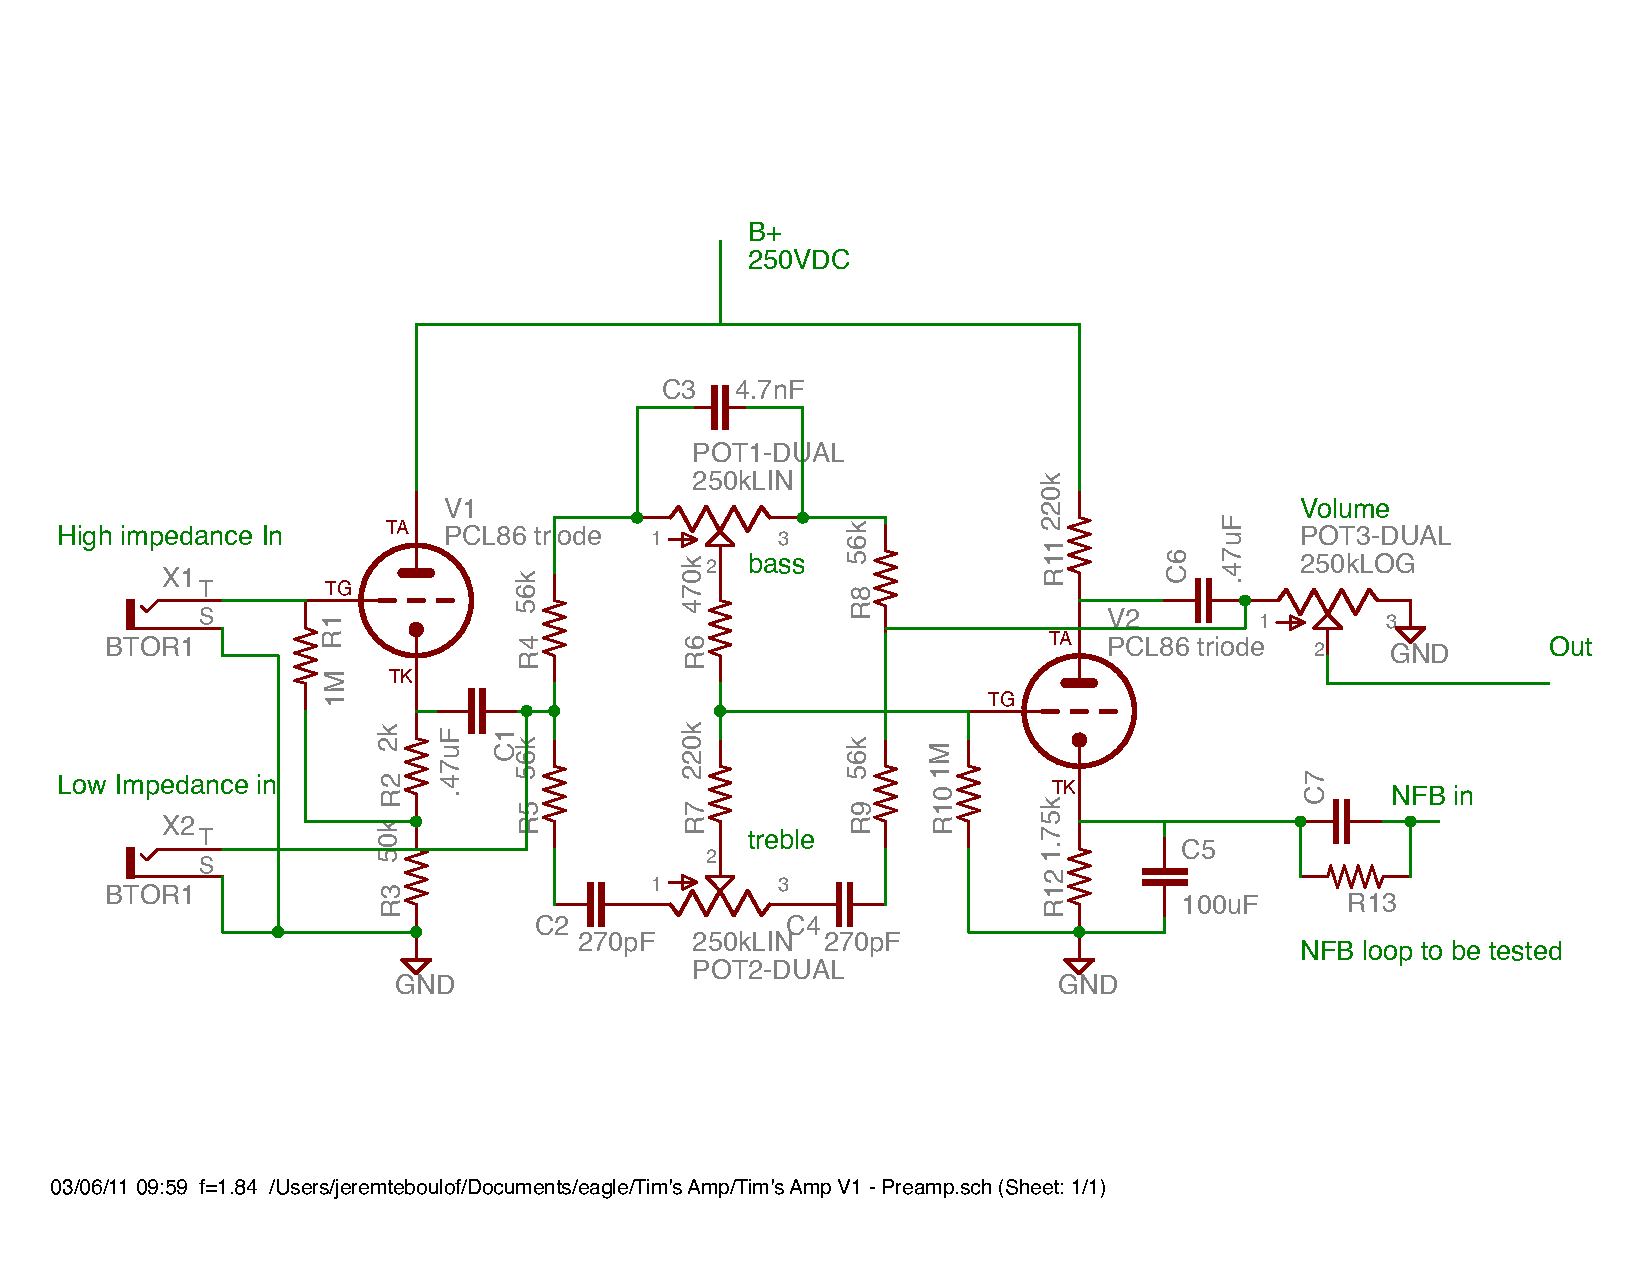
\includegraphics[width=1\textwidth]{timsamp}
\end{figure}

\begin{figure}[h!]
  \caption{bill of materials for that preamplifier}
  \centering
    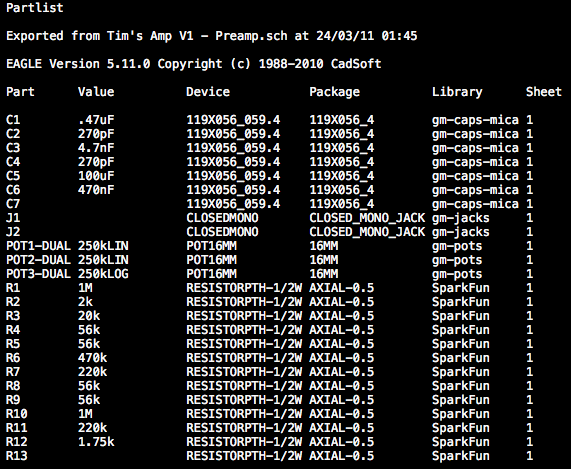
\includegraphics[width=1\textwidth]{bompre}
\end{figure}

The ubiquity of digital devices today cannot be overstated. This is particularly true in musical devices - the versatility of artistic computing is discussed at length by musicians in the upcoming chapters. 

Software design offers a rich tradition of experimentalism for audio. Max Mathews acts as the forefather of a long line of extensively-studied composers who either programmed their own instruments, or worked closely with engineers to do so. Those efforts effectively redefined the world of electronic music, and as we'll see excluding digital from a discussion of contemporary audio hardware in music would be as toxic as it would be difficult. Open source originates in software- this thesis wishes to expose the possibilities of interdisciplinary design approaches. 

	By looking at the role of experimentalism in electronic music hardware, one can get a sense of how hardware can complement the speed of innovation that characterizes software. Improving physical music devices can take three forms:  
	
\begin{itemize}
	
\item component innovation

\item system innovation 

\item interaction innovation  

\end{itemize}

Historically, electrical engineers have been concerned with those first two points, while the latter is more open to interpretations from various sources. The New Interfaces for Musical Expression (NIME) conference has developed out of a desire to unite efforts in that field. Software affects all three levels, blurring the distinction between component and system while re-labeling interaction design as UX/UI design (user experience/user interface). 

Looking at the historical development of those three types of innovation in electronic music and electronics gives us a better sense of where the field is today. 

\section{Electronic music as invention}

	Before 1915 and the beginning of commercially available vacuum tubes, electronic music relied on a spirit of adventure and experimentalism close to the later works of Tudor, Kuivila, Collins and Ghazala. Dunn's pioneers developed system because they invented or developed interesting forms for the basic components of an electronic circuit (the resistor, the capacitor, the inductor). 
	
\paragraph{Thomas Edison}

	\begin{figure}[h!]
	  \caption{one of Edison's ``Tone Tests'', 1918 \cite{thompson1995}}
	  \centering
	    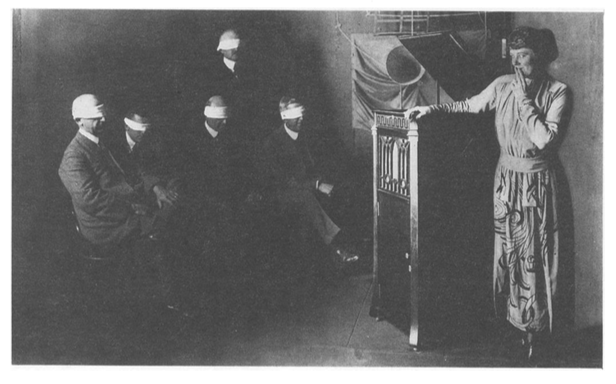
\includegraphics[width=.5\textwidth]{tonetest}
	\end{figure}
	
Edison was, in addition to his involvement in the electrification of western countries in the early 20th century, an accomplished inventor and tinkerer. The phonograph he toured to advertize in the United States through \emph{tone tests} emphasized the intelligibility of the voices it reproduced. Although critics pointed out the impressive but imperfect reproduction from the device, Edison maintained that they couldn't accurately distinguish one from the other \cite{thompson1995}. 

There could not have been a better link between Aristotle's acousmats and Schaeffer's listening techniques - and this context sets the framework within which electricity and music would live up to this day. It is difficult to imagine or think of the synthesized without referring to the ``natural'', almost as it is easy to disregard the point or the honesty of electronic instruments. And yet, purely electrical instruments developed. Whether by accident, rigorous research, or haphazard guesses, the early inventors of electronic music were also trying to convince others that their work was, at the very least, asking interesting questions. 
	
\paragraph{C.G. Page}

	C.G. Page “toyed” with horseshoe magnets, spools of copper wire and batteries - in 1837, he would publish one of the first reports of electronic sound, which he called galvanic music without being able to explain it \citep{page1837}. 
	
\paragraph{Elisha Gray}

	Elisha Gray, in 1874, was the first electronic musician to tour his home country. His invention, the musical telegraph, was invented after he realised he could control the pitch of the hum produced by a vibrating metal strip attached to his bathtub while running experiments with his nephew. After touring once with it, he ignored its musical potential and failed when he attempted to use a modified version of the device as an early iteration of what would then become the multiplexer \citep{holmes2002}. 
	
	\begin{figure}[h!]
	  \caption{Gray's Electro Harmonic Telegraph patent}
	  \centering
	    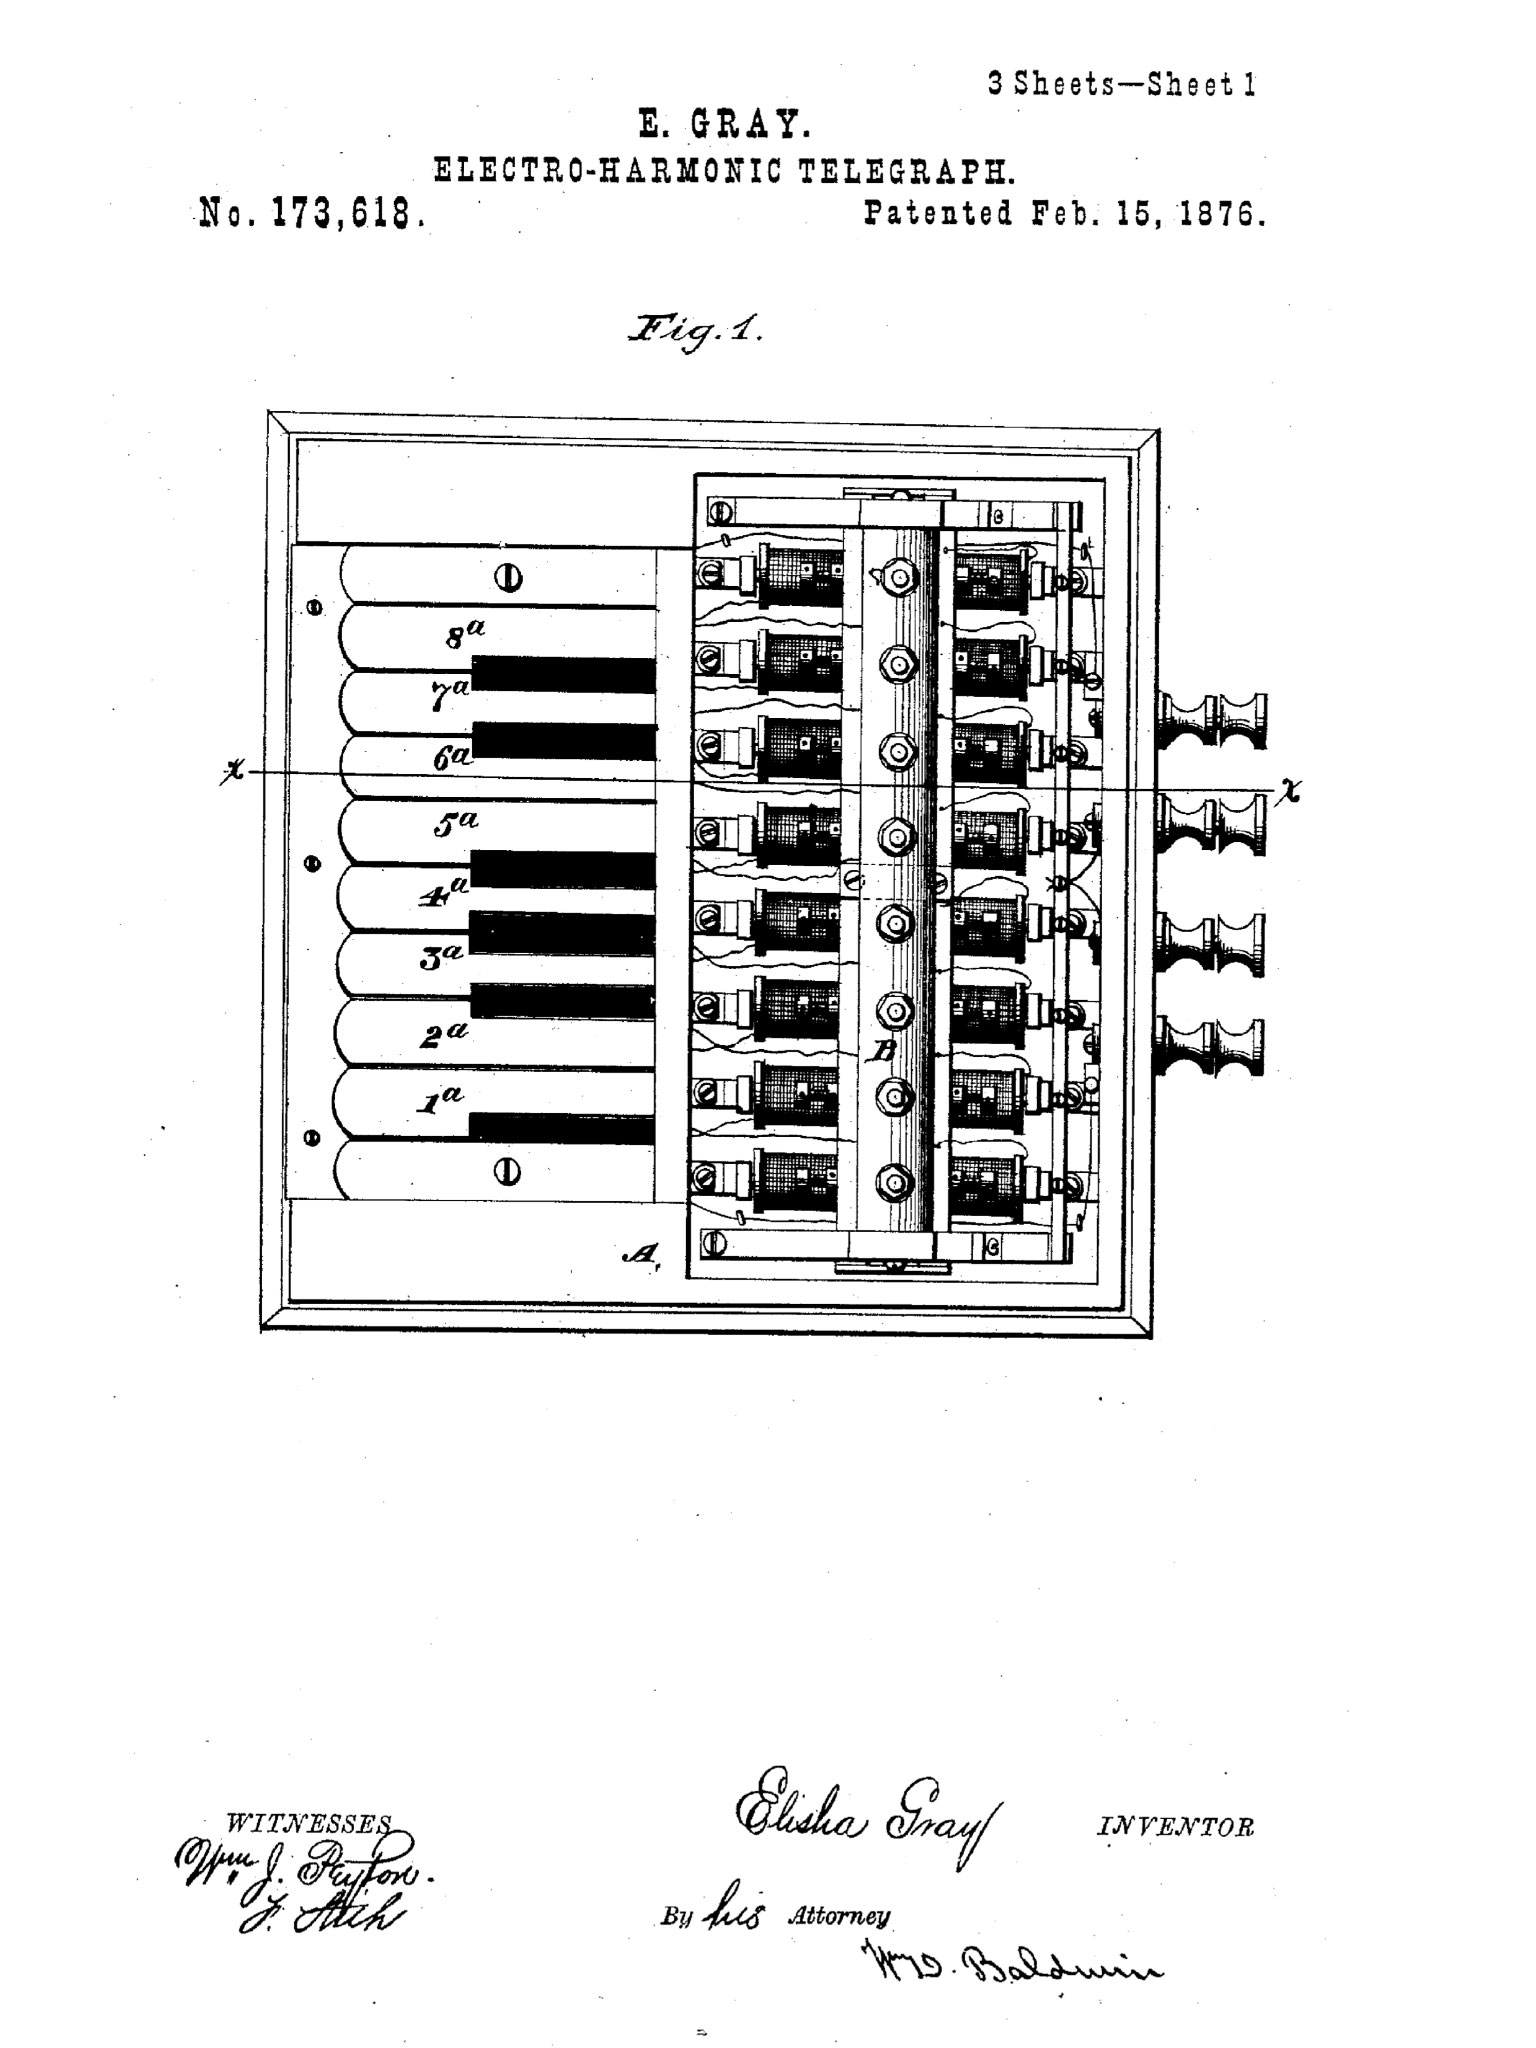
\includegraphics[width=.5\textwidth]{mustel}
	\end{figure}
	
\paragraph{William Dudell}

	William Duddell’s 1899 ``singing arc'' offered pitch control for the audible hum of carbon-arc light bulbs. Here again, the musical application was coincidental - he was originally trying to get rid of the unwanted buzzing sound \citep{nasmyth1908,holmes2002}. 
	
	\begin{figure}[h!]
	  \caption{Illustration of the singing arc}
	  \centering
	    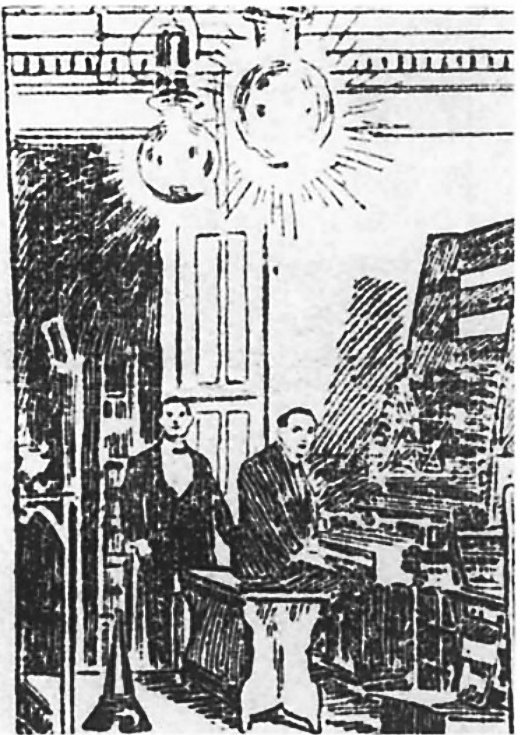
\includegraphics[width=0.5\textwidth]{singarc}
	\end{figure}

\paragraph{Thaddeus Cahill}

	Thaddeus Cahill’s Telharmonium, patented in 1896, was the first successful massive undertaking of electronic music hardware. In its full form, the two-hundred ton instrument was a sophisticated electro-mechanical polyphonic instrument, developed and assembled for the sole purpose of entertainment. With Cahill rises the persona of musical inventor as businessman, effectively becoming one of handmade electronic music’s earliest father figure \citep{holmes2002}. 
	
	\begin{figure}[h!]
	  \caption{Some of the Tellharmonium's tonewheels}
	  \centering
	    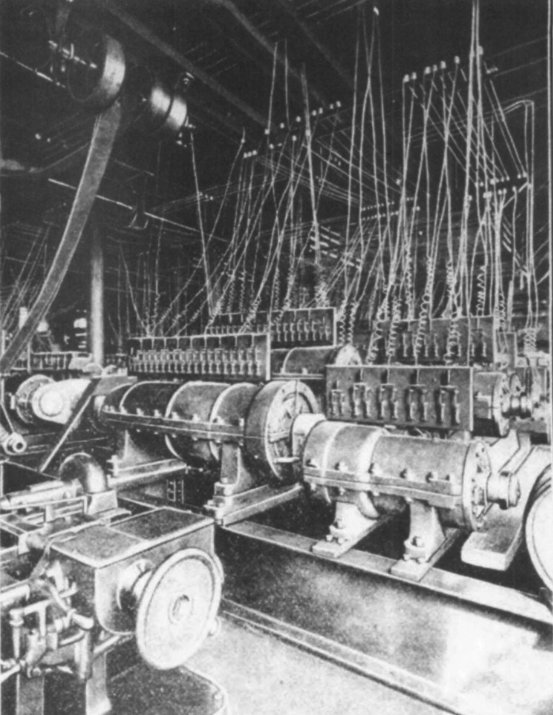
\includegraphics[width=0.5\textwidth]{dynamo}
	\end{figure}

	This short list describes only some of the inventors who were much comfortable with raw materials and physical experimentation than most of today’s electro-acoustic or digital music community. Interestingly enough, none of the signal generation methods described above (electromagnetic oscillation, RLC-circuit oscillation, spark-gap oscillation, electromechanical oscillation) are common in the following generations of electronic music hardware experiments. 

	With electronics still in their infancy - no design tradition, few formal structures -  experimentation is the only option. By operating in an effectively anelectronic context, Cahill and his peers established the baseline for electronic creativity. This is the origin of electronic music, where the promise of the new medium was enough for people to blindly experiment. 

\section{Electronic music as an institution}

In the period following the first world war, the popularization of radio went with the development of not only standardized parts, but also of hobby electronics. It was more cost-effective to buy a kit and build a radio yourself rather than purchase the completed product. In 1922, a Freshman “masterpiece” radio cost \$17 as a kit, while a completed set cost \$60. This corresponds to \$240 v. \$850 in 2014 (radioblvd.com, w2014; data.bls.gov, w2014). 

	\begin{figure}[h!]
	  \caption{advertisement for the Freshman radio kit}
	  \centering
	    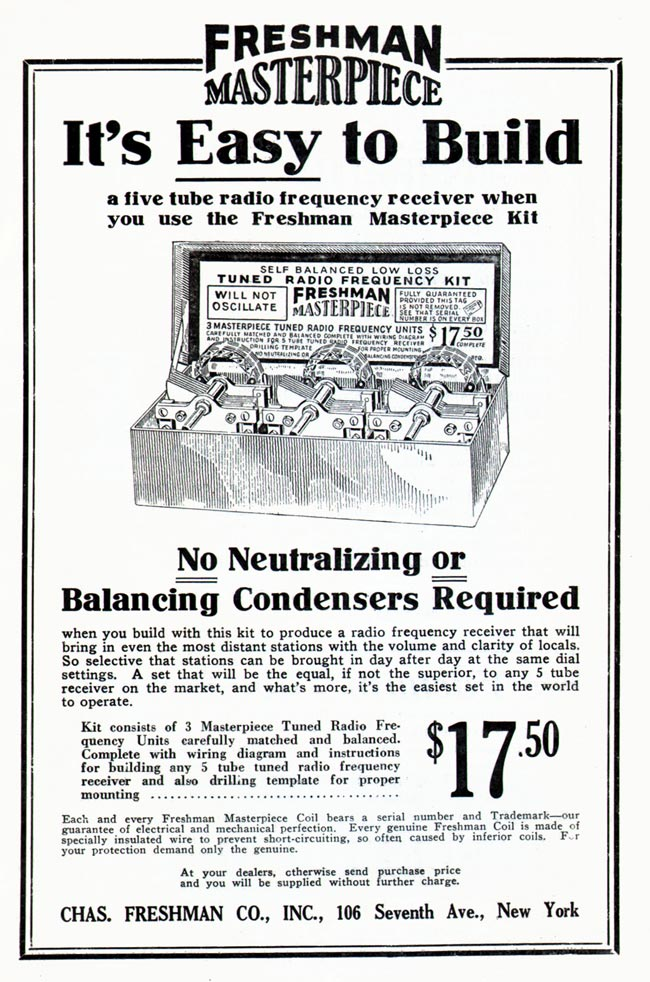
\includegraphics[width=.5\textwidth]{freshman}
	\end{figure}

This was facilitated in the U.S.A. by companies like Radio Shack and Allied Electronics. Both companies, amongst many, sell the parts - resistors, inductors, capacitors, transformers, tubes - and the tools necessary to assemble a variety of consumer audio and radio electronics. 

Radio Shack’s first catalog (w2014) from 1939, contained 80\% kits, parts and tools and 20\% completed products. The increasing availability of parts and tools solidified after the second world war, with catalogs like Radio Shack’s growing from 1939’s 72 pages to 110 in 1946. Heathkit, a major electronics kit focused on high fidelity audio and radio equipment, was founded in 1947. Popular Electronics \#1, which compiled articles on those kits and the various technological developments available to the patient home-builder, was published in 1954. 

	\begin{figure}[h!]
	  \caption{Front cover of Radio Shack's 1939 catalog}
	  \centering
	    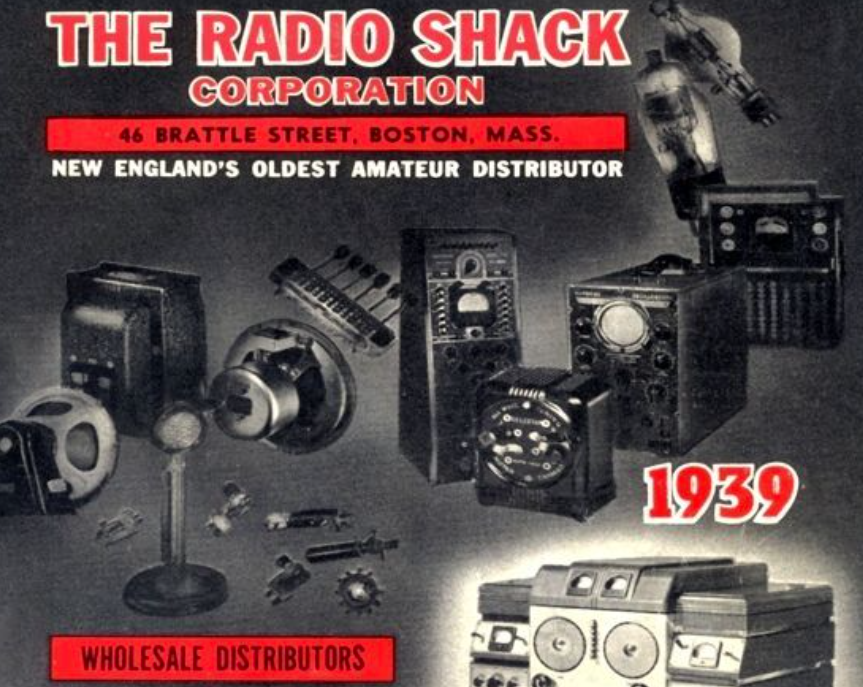
\includegraphics[width=1\textwidth]{radioshack}
	\end{figure}

This resulted in a generation of engineers and musicians growing up with electronics, who were both eager to take advantage of the relatively positive post-war atmosphere \citep{holmes2002}. The father of a certain Robert Moog, whom we will discuss in an upcoming section, was one of the first American amateur radio operators \cite[p.12]{pinch2002}. 

At that time, signal processing was one of the main research areas in the thriving field of electrical engineering. The 1953 edition of the Radiotron Designer's Handbook \citep{langford1953} dedicated a third of its 1500 pages to audio electronics. Schematic, tools, methods and designs are optimized, thoroughly investigated and standardized. Building off their industrial successes, Institutions serve as the breeding ground for most renowned artistic applications of technology. This results in the emergence of the French (ORTF), German (WDR), and Italian (RAI) experimental music studios, all housed by public radio stations. In the U.S., RCA and Columbia University composers collaborated to develop the RCA synthesizer, closer to the telharmonium in scale than anything in the first half of the 20th century. Max Matthews, after being trained as a Navy radio repairman, found work at Bell Labs with music enthusiast John Pierce, whose fostering would mark the beginning of computer music \citep{park2009}. Most of the technology used in those musical systems was a byproduct of the war research effort: it seems natural for the first wave of artists and designers to be involved with those organizations \citep[p.81]{holmes2002}. 

	\begin{figure}[h!]
	  \caption{the RCA Mk.II with its inventors}
	  \centering
	    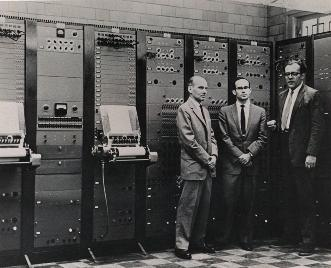
\includegraphics[width=.5\textwidth]{rcamkii}
	\end{figure}

\paragraph{Hugh Le Caine}

Hugh Le Caine’s Electronic Sackbut and its concept of voltage-control proved to be an inspiration for the Moog, and a foreshadow of most electronic music systems. Started in 1945, he worked on the monophonic system until 1971, by which time it possessed two important characteristics: 
\begin{itemize}
	\item the oscillator could be modulated in both timbre and pitch. Furthermore, some settings would create unpredictable variations. Those changes were done through the earliest implementation of voltage control. 
	\item the interface of the instrument allowed for expressivity and ease of use still difficult to achieve today: the piano keys could move side to side to control vibrato, and sense how hard they were pushed down to control amplitude. The left hand that controlled the oscillator parameters did so in way that was particularly rapid to become accustomed to \citep{holmes2002}. 
	
	The Sackbut was a voltage controlled monophonic instrument with specific timbral controls and effective gestural mapping that incorporated controlled amounts of uncertainty. Although it was a failed commercial endeavor, voltage control and touch-sensitivity would emerge in the fifties and sixties as essential components of synthesizers, while impredictability or uncertainty in an instrument would be the concern of Tudor and his cohort. Le Caine sets the example for originality and independence within the institutionalized practice of electronic music and electronic instrument design\cite[p.147]{holmes2002}. 

	\begin{figure}[h!]
	  \caption{Le Caine's Electronic Sackbut}
	  \centering
	    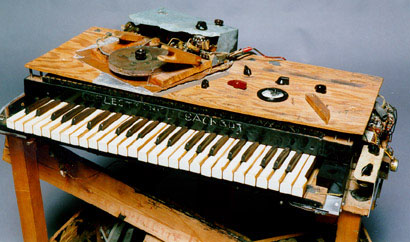
\includegraphics[width=1\textwidth]{sackbut}
	\end{figure}

Le Caine's Sackbut is in the direct continuation of Dudell's experiment - crude electronics combined with the familar keyboard interface. Thoroughly independent research in audio synthesis at the time is limited, but two interesting instances can be presented: 

\paragraph{Raymond Scott}

Raymond Scott was a self-taught hobbyist with the additional motivation, funds and time provided by his successful career as a composer of electronic music for commercials. Having independently developed one of the earliest multi-track tape recorders (7 to 14 tracks), amongst a number of other inventive projects, he would also ultimately receive visits from an impressed Robert Moog. However, he would fail to turn his technological expertise into a successful business. 

As a designer of personal electronic music systems, Scott's vision was most condensed in his \emph{Electronium}. The device is described as being a self-composing device that could be influenced by the user \citep[p.142]{holmes2002}. He sais of the apparatus that is not a synthesizer, as it has not keyboard. By inputting a theme through the hundreds of knobs, permutations on that theme are generated and played - when a satisfactory iteration is produced, the user could activate the record mode and the system would compose independently. ``...the Electronium adds to the composer's thoughts, and a duet relationship is set up between man and machine'' \citep{chusid1999}. The Electronium ``is not played, it is guided''\citep{darter1984}. The device in effect included an analog sequencer and algorithmic composition system, both of which could function together by 1960. 

	\begin{figure}[h!]
	  \caption{Mark Mothersbaugh bought the only electronium from Motown and is restoring it}
	  \centering
	    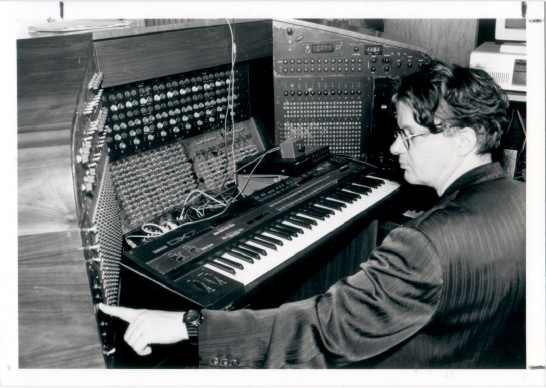
\includegraphics[width=1\textwidth]{electronium}
	\end{figure}
	
Scott's Electronium is an interesting example of independent workers who built off an interest and expertise in science and engineering to push the boundaries of what could musically be done with the available technology. His notorious paranoia with regards to sharing the design (even his attempt at patenting the device failed because of a technicality) meant that little came out of his innovation. From a design perspective, Scott built on the information available to him as a composer and recording engineer to develop his instruments without the technical or financial support of an institution. This is an example of how shared information can still produce advances in instrument design, regardless of whether or not discrete products are shared as well - the open source ecosystem is a robust mechanism that can survive even if it remains static. 

\paragraph{Louis and Bébé Barron}

Louis and Bébé Barron provided soundtracks for films such as 1956’s Forbidden Planet. They were innovative in their implementations of vacuum-tube based synthesis, creating systems based on equations from a cybernetics book by Norbert Wiener. They would describe the resulting devices as ``alive'', an interesting parallel with Scott’s Electronium. In the tradition of Duddell and Gray, the circuits that Louis built were accidently overdriven and eventually failed. These decaying sound processes would be used as the basis for their composition, which they assembled in a way similar to Schaeffer’s concrète process \citep{dunbar2010}.

	\begin{figure}[h!]
	  \caption{Louis and Bébé Barron in the studio}
	  \centering
	    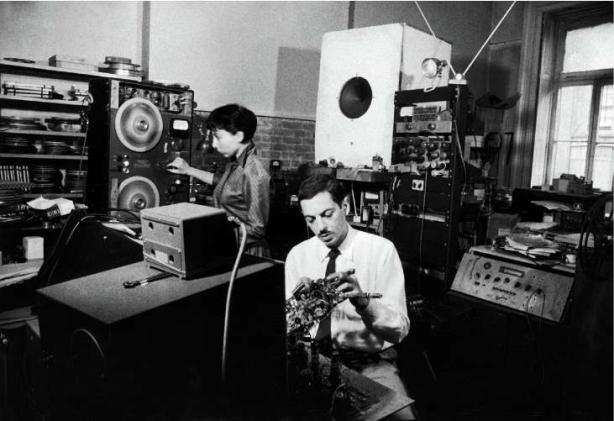
\includegraphics[width=1\textwidth]{barrons}
	\end{figure} 
	
The Barron's and Scott's work, although not immediately influential in terms of instrument design, appear in hindsight as symptoms of the artistic need to tinker and experiment with the concept of electronic music devices as more than tools, but honest instruments if not full-blown artificial composers. Echoes of this intuition will be visible in chapters 3 and 4, as some contemporary practitioners describe there designs as the other half in their musical duets. 

That concept would be explicitly and perhaps more visibly developed by a set of avant-garde musicians in New York City, Michigan and the american west coast. 

John Cage’s experiments throughout the 50’s would incite his collaborator David Tudor to abandon the piano that brought them together in favor of an experimental approach to music through homemade electronics \citep{holzaepfel1994,collins2004}. Unlike our two previous examples, however, Tudor and Cage would have strong affiliations with academia and indirectly, industry. 

As musical systems beneficiated from technological advances developed by the military and major research bodies, fewer people were operating independently with enough success to be documented. Work during the vacuum tube age had undeniable impact: Stockhausen, Schaeffer, Oram, or the Columbia Music Center stand as landmarks in the development of experimental music, arguably solidifying the field as a worthy academic pursuit. However, their efforts were out of the public's possibilities, and often, technical grasp. From a design standpoint, one could describe the ORTF, RAI and WDR studios, as well as the RCA Mk2 as fitting within Dunne's concept of the optimal: an efficient, versatile machine. 

\section{electronic music as a living system}

\subsection{Tudor and Cage: electronics speak for themselves}

	Before being within the reach of the general public, electronic music instruments had to find an audience in that public. In that process, two converging trends contribute to our next development. 
	
	First, the avant-garde continues its exploration of technological possibilities, while reconsidering its limitations and preconceptions. Variations II is a 1960 piece by John Cage, “the greatest degree of abstraction of a compositional and notational model that Cage developed over the period from 1958 to 1961.”
	
\begin{figure}[h!]
  \caption{An instance of setting the score for Cage's \emph{variations II}}
  \centering
    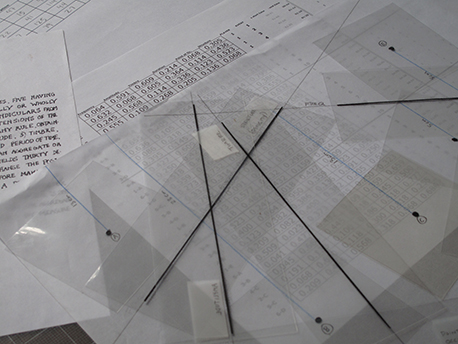
\includegraphics[width=1\textwidth]{variationsii}
\end{figure}
	
	 It was extensively studied, then performed in 1961 by David Tudor, for whom Cage effectively wrote the piece. The extent to which the work was internalized by Tudor has led to some to consider him as the piece’s co-composer \citep{pritchett2004}. It included the use of a complex system of signal processing electronics, designed to implement some of Cage’s ideals of compositional indeterminacy. “You could only hope to influence the instrument”, said Tudor in describing his use of the device \citep{nakai2014}. 
	 
 	\begin{figure}[h!]
 	  \caption{Tudor performing Variations II}
 	  \centering
 	    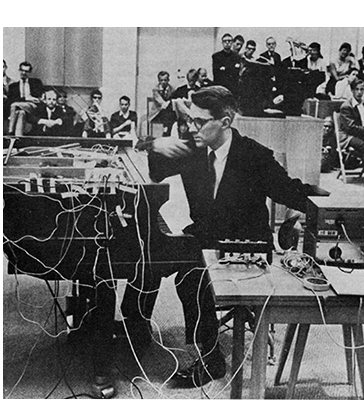
\includegraphics[width=0.5\textwidth]{tudorvar}
 	\end{figure}

Tudor’s debuts are not independent of public or private groups. Fluorescent Sound is commissioned in 1964 by Robert Rauschenberg and sees its sole performance in Stockholm’s Moderna Museet. \emph{Bandoneon!}, his second piece, premiered in 1966’s Nine Evenings of Theatre and Engineering. Instigated by Rauschenberg and facilitated by Bell Laboratories, this event gave artists from the american avant-garde a chance to collaborate with some of the world’s most productive engineers in New York’s Armory building \citep{kuivila2004}. The collaboration would prove instrumental in fostering the experiments in art and technology (EAT) series. 
	
Reminiscent of Barron’s living circuits, Tudor described his second piece as “composing itself out of its own composite instrumental nature.”  \citep{tudor,kuivila2004}. Tudor, through various collaborations, develops an affinity for circuits which ultimately make some of the compositional decisions themselves. 

Cage had been using electronics in performance since the late 30’s, with pieces such as the Imaginary Landscapes series or 1959’s Water Walk. Reich’s 1965 It’s Gonna Rain proved that process-based composition rooted in solely in technology held musical value. Tudor, with his implementation of Variations II, Bandoneon!, and the Rainforest series, legitimizes a compositional approach based explicitly on materiality. “The objects should teach you what it wants to hear”, he states after performing Rainforest IV (1973). Cage will echo the statement in 1987 with the following response: “the components, the circuitry is the music, and it comes alive when it is performed” \citep{nakai2014}. 

Tudor was in a unique position of artistic experience and legitimacy that enabled his experiments to become regarded as groundbreaking and foundational \citep{collins2004}. Through collaborations with Gordon Mumma, David Behrman, Hugh Le Caine, John Fulleman, and John Driscoll, and thorough personal investigation, he gathered enough experience to masterfully implement one of the first documented uses of chaotic electronics in music \citep{kuivila2004}.  Like Cage, he would not be attached to the idea of considering himself a composer \citep{kuivila1998}. Tudor is the model for multiple generations of hobbyists, independent scholars and experimenters who situate themselves somewhere between self-taught artistic systems designer and musician. 

A common thread in Tudor’s work was the spotlighting of electronics customarily hidden during performances, \"composing inside electronics\" ~\ref{appendixA}. In trying to take advantage of the sculptural aspects of the instruments through sonification by using contact microphones or transducers, his work also developed a notion of sound art which challenges the distinction between installation and performance \citep{driscoll2004}. His approach was different from Lucier’s: where the latter focuses each piece on a specific physical phenomenon, Tudor’s work was rarely concerned with minimalist systems \citep{collins2004,driscoll2004}. 

	\begin{figure}[h!]
	  \caption{Performing amidst electronics for \emph{Bandoneon!}}
	  \centering
	    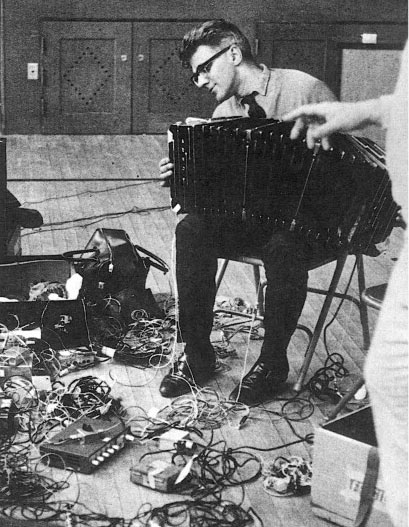
\includegraphics[width=0.5\textwidth]{tudorband}
	\end{figure}

Another manifestation of his originality was his coercion of general-purpose abstraction borrowed from electrical engineering, then adapted for the performance of his pieces and equipment \citep{kuivila2004}. This repurposed set of abstract notations would blur the line between schematic and score, just like Cardew and Earle Brown proposed the use of abstract art as basis for musical performance. In doing so, his performances became more and more personal - Tudor’s oeuvre is “practiced, not preserved” \citep{kuivila1998}. This “musical practice based on constant modification and innovation” \citep{driscoll2004} is a direct foreshadowing of the methods which define online do-it-yourself communities active today. 

	\begin{figure}[h!]
	  \caption{Tudor's diagram for his \emph{Rainforest IV} in effect describes the piece}
	  \centering
	    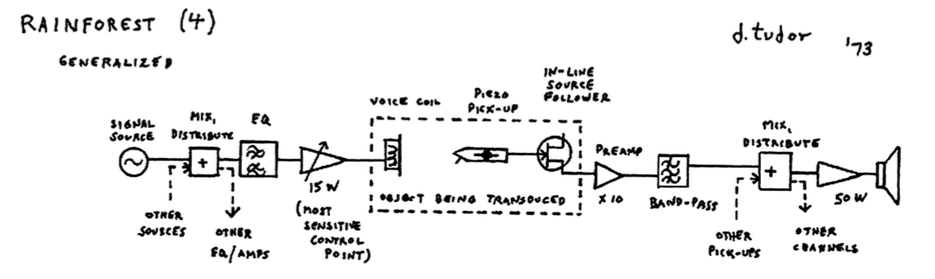
\includegraphics[width=1\textwidth]{rainforest4}
	\end{figure}

	\begin{figure}[h!]
	  \caption{Tudor's score for \emph{Untitled}}
	  \centering
	    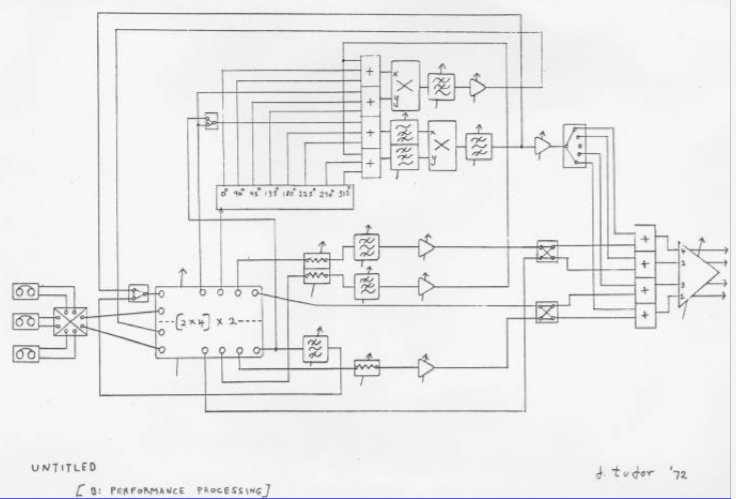
\includegraphics[width=1\textwidth]{untitled}
	\end{figure}

If Tudor defined a practice of experimental electronic music systems that complements Cage’s sonic uncertainty, it is largely thanks to semiconductors (Collins, in\ref{AppendixA}. Transistors and integrated circuits offered the functionality of vacuum tubes without the latter’s size, weight, price and high voltage hazards. These became commercially available and well documented as he started using custom electronics \citep{collins2004}, with Texas Instruments selling their first silicon transistor in 1947 (texas instruments, w2014) and integrated circuits (ICs) becoming available in the 1960’s.  

The easily replaceable, cheaper components would make prototyping musical electronics more accessible, also allowing Tudor to easily enroll help for performances. Starting with 1973’s performance of Rainforest IV, his group of collaborators would solidify as the Composers Inside Electronics group (C.I.E., w2014). The group, reformed for Tudor’s death in 1996 is still active today. Their approach is resumed by Tudor in 1976: 

\begin{quote}
						
Electronic components and circuitry, observed as individual and unique rather than as servomechanisms, more and more reveal their personalities, directly related to the particular musician involved with them. The deeper this process of observation, the more the components seem to require and suggest their own musical ideas, arriving at that point of discovery, always incredible, where music is revealed from ``inside,'' rather than from ``outside.'' \citep{tudor1976,nakai2014}

\end{quote}

Tudor’s innovative methods and C.I.E.’s ever growing cast have guaranteed the relevance of their work in scholarship of musical hardware leading up to the current decade \citep{collins2004,collins2006,collins2008,collins2010,nakai2014,driscoll2004,kuivila2004}. Through the learning, supplying and sharing tools offered online, Tudor’s ideals of experimentation and collaboration have come to be more relevant and accessible than ever. As the E.A.T. experiments failed, the public's appreciation and understanding of overwhelmingly complex electronic art fell \citep{burnham1979}, giving some of the stage to artists who managed to blend adventurous electronics with popular traditions. Voltage control and modular systems became commercially available, giving some leeway to the talented but reclusive experimenters that had not become engineers for Bell Labs or European studios. 

\subsection{The rise of voltage control}

With the development of solid state electronics, audio signal synthesis and processing becomes a more manageable endeavor. As Hugh Le Caine intuited and implemented, but failed to popularize, signals could serve both as raw audio signal or as control information for paramaters of that audio signal. 

Bob Moog, building off of the experience he accumulated assembling, selling and distributing theremin kits, develops that capability in an expensive but publicly available package: the Moog modular synthesizer. Each module serves a primary function and communicates with other modules using those formatted control voltages. The parallel with computer music is straightforward: unit generators are the equivalents of voltage control oscillators (VC0) and their low frequency equivalents (LFO), ring modulation is multiplication, add/substract units are mixers, etc. 

	\begin{figure}[h!]
	  \caption{A schematic for the minimoog's VCO circuit, along with a rough circuit board layout}
	  \centering
	    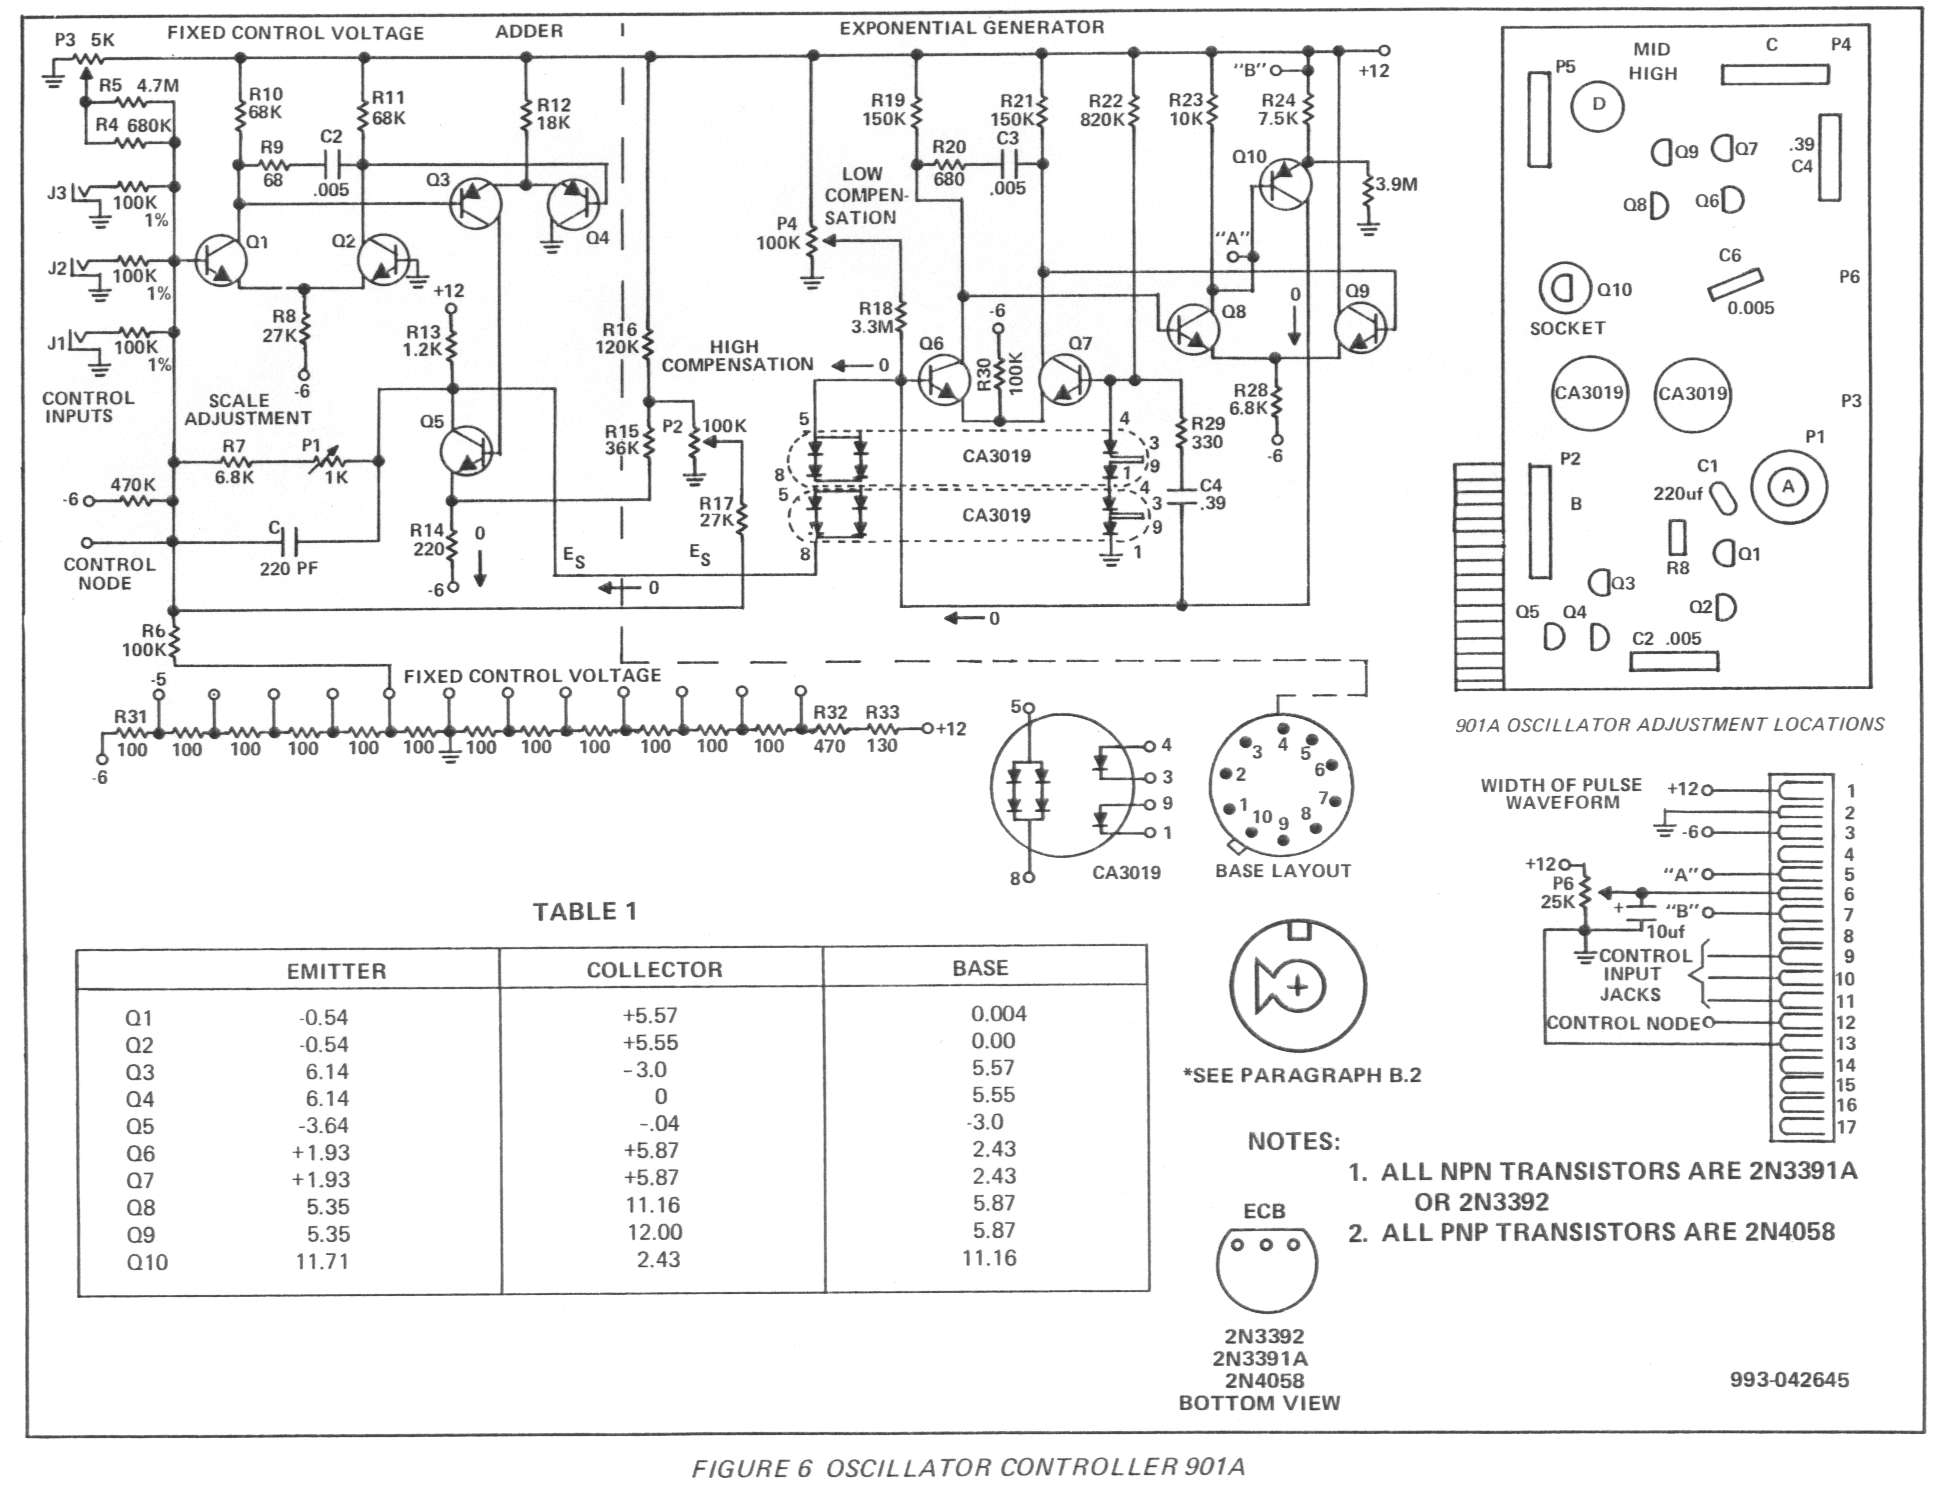
\includegraphics[width=1\textwidth]{minimoogVCO}
	\end{figure}

One can see in the commercial modular synthesizer a first opportunity for the public to ``build'' personalized instruments for popular music. Although the number of modules is limited (not to mention the prohibitive cost), the end user is responsible for the final layout of their device. 

	\begin{figure}[h!]
	  \caption{Klaus Schulze's moog-based system, mid 1970's}
	  \centering
	    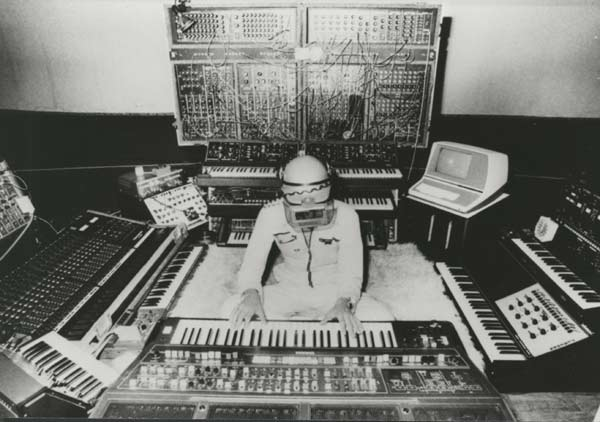
\includegraphics[width=1\textwidth]{schulze}
	\end{figure}

Although Moog is not the only manufacturer of modular systems, the quality of his system, his choice to pair his devices with the more musically familiar keyboard and some public relations skills make him the bridge between classical tape and electronic composers. What Wendy Carlos sees as the tools of ``ugly music'' can now be used for ``appealing music you could listen to.'' \cite[p.169]{holmes2002} As Carlos fine-tuned her own Moog system, she eventually went to get a custom version of the system made to her specifications. 

	\begin{figure}[h!]
	  \caption{Carlos and her Moog 55 system}
	  \centering
	    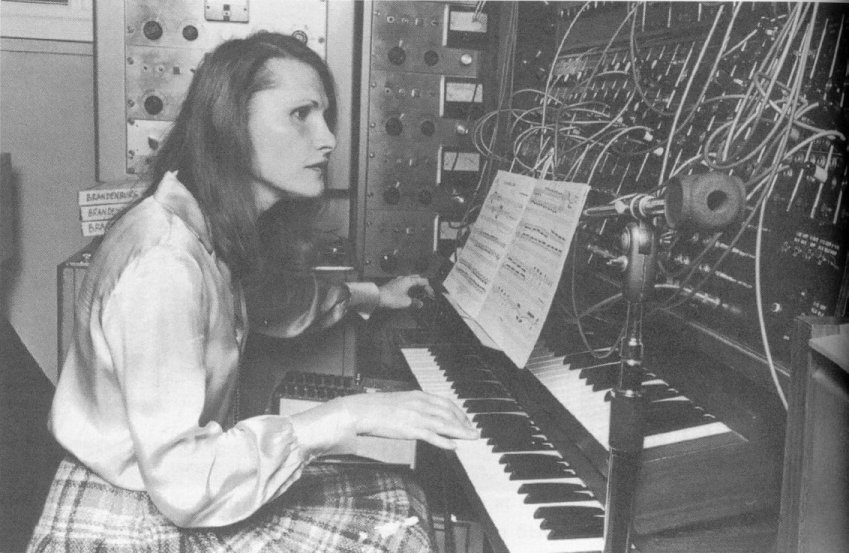
\includegraphics[width=1\textwidth]{carlos}
	\end{figure}

A number of other musically inclined inventors also developed comparable systems, each with their own specificities. Two American complements to Moog are Serge Tcherepnin, designer of the Serge modular system, and Donald Buchla, responsible for the Buchla synthesizer. The latter is most relevant in our discussion. 

As mentioned in the introduction, Buchla viewed himself as a luthier, designer of instruments, rather than the engineer of machines \citep{pinch2001}. His decision to develop new methods of interacting with his circuitry rather than relying on pre-existing schemes like Moog's keyboard severely limited his user-base, but the quality of his luthery would ultimately appear as inspiring for circuit designers up to today \citep{rylan2015}, \ref{AppendixA}. ``The Buchla box was designed for musicians who wanted to produce a complex piece of music in real time.'' \cite[p47]{pinch2002}. If Moog's modular model is the template for much of the additive synthesis audio software and hybrid hardware today, Buchla's interface and interactive system design work are still being digested and re-used. 

	\begin{figure}[h!]
	  \caption{Buchla's distinctive arbitrary function generator (recent model)}
	  \centering
	    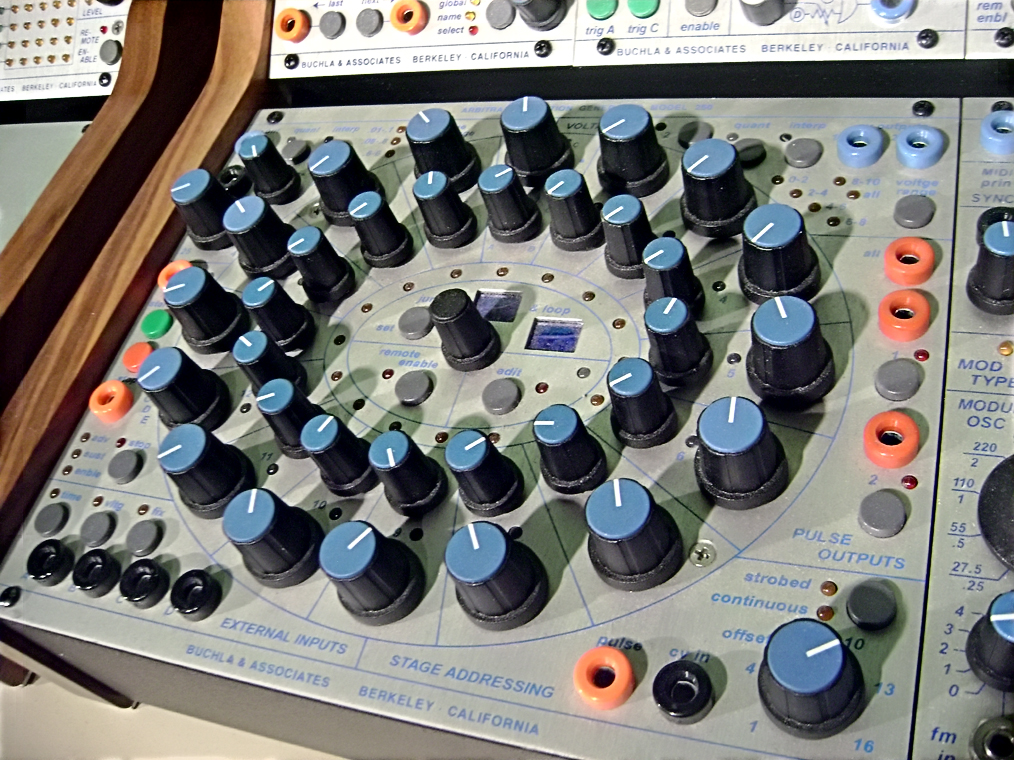
\includegraphics[width=1\textwidth]{buchlaarb}
	\end{figure}

Ultimately, Pinch concludes: ``Designers `script' or `configure' ideal users into their machines.(...) Scripts try to contain the agency of users, but users can exert agency, too, and can come up with their own alternative scripts." \cite[p.311]{pinch2002}. The complex interplay between designer and user takes on a significantly different meaning when those two personas belong to the same person. In that sense, being both the designer of the system and the user allows for more varied processes to emerge, as well as a more original set of parameters for those processes. The ease with which tools permit this dual role directly influences the variety of the instrument design ecosystem and its evolution cycles. 

\subsection{Brian Eno: uncontrolled versus unintentional realizations of music}

A prime example of avant-garde, personal electronic music techniques coming to a popular forefront with relatively little technical support is the British composer Brian Eno and his development of the system later known as \emph{Frippertronics}. His process on \emph{Discreet Music} is clearly related to Tudor's: 

\begin{quote}
	If there is any score for the piece, it must be the operational diagram of the particular apparatus I used for its production. \citep{eno1975}
\end{quote}



\begin{quote}

even though it is correct to say that composing process music does not require electronics, the use of electronic instrumentation often inspires its creation. The very nature of electronic music instruments, old and new, encourages a composer to think in terms of a process, whether that process is a hardwired patch of cables, a virtual patch inside a computer, or the turning of dials to various increments that shape the development of a piece of music. \cite[p.237]{holmes2002}

\end{quote}


If Tudor operated between the component and system levels, Eno is somewhere between system and interaction. However, Tudor's wish to see personality emerge from circuits is echoed by Eno's  ``acceptation of that passive role'' which characterizes the first half of \emph{Discreet Music}. 

This record allows us to briefly discuss the role of intentionality in composition with autonomous or semi-autonomous musical systems. If Eno's practice at that time is implicitly linked to Tudor's, he is also explicitly acknowledging the unintentional nature of his process: 

\begin{quote} ... having laid down, I realized that the amplifier was set at an extremely low level, and that one channel of the stereo had failed completely. Since I hadn't the energy to get up and improve matters, the record played almost inaudibly. This presented what was for me a new way of hearing music - as part of the ambience of the environment.
	
	\citep{eno1975}
	\end{quote}

He combined this new vision of Satie's \emph{Furniture Music} \citep{satie} with an interest for tape-loop based delays dating back to the previous decade, creating the following system: 

\begin{figure}[h!]
  \caption{Operational Diagram for Discreet music}
  \centering
    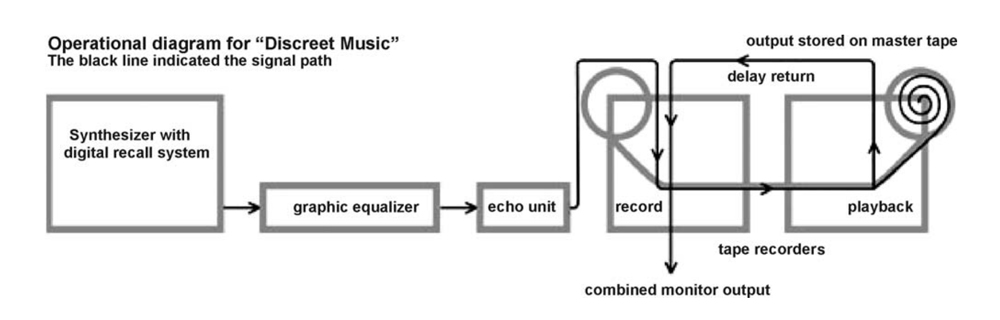
\includegraphics[width=1\textwidth]{discreetdiagram}
\end{figure}

Eno would keep combining this approach to listening with evolved versions of this 1975 system, eventually yielding elements of the \emph{Ambient} series \citep{eno1978,eno1980,eno1980b,eno1982}. This also developed beyond the studio: if \emph{Discreet Music} was originally intended as a backing track for improvisations by Robert Fripp, the latter would eventually use the system extensively through to this day. \emph{Frippertronics} is both a performance, composition and installation medium, a flexible, adaptive and personalized instrument.  

The compelling nature of this release is undeniable. \emph{Discreet Music } holds high value as a prototypical ambient record, an instance of hardware-based process music, and an example of a semi-autonomous electronic music instrument. If Tudor blurred the line between composition and performance through his interpretation of Cage and subsequent live electronics works, Eno's work develops this further by legitimizing curated unintentionality as a compositional prompt. 

More so than Tudor's various devices, \emph{Frippertronics} serve as the archetype of personal electronic music instruments. It illustrates the amount of resources, technical knowledge and musical intuition and luck necessary to make the medium of electronic music one's own. 

At this point, it seems valid to hypothesize that when the ``ideal user'' is the designer, some tend to create systems that have a capacity for independently creating musical material. This hypothesis will be discussed in the upcoming section and chapters.  

\section{Elecronic sound as craft} 

	Tudor as a composer would be largely ignored until his death [Collins, app.A]. As a teacher, he had tremendous impact on what technically inclined artists should or could do. 
	
\subsection{Paul DeMarinis}

Paul DeMarinis worked on the electronics of the 1973 Rainforest IV installation. This period of cohabitation with Tudor's generation of collaborators (John Cage, Robert Ashley, David Behrman) proved to be a formative experience for the Mills College graduate student. Having described them as ``incredibly generous'', they gave him an appreciation of audio electronics that proved to be original for his time. By 1973, he said, ``I wasn't interested in building synthesizers. I was much more interested in building pieces.'' \cite{ouzounian2010}
	
	His first major solo work, the \emph{pygmy gamelan}, has severel important defining features: it was generative, pulling noise from background radiation to produce shifting five-note melodies. It used a combination of early digital and analog ICs, and finally, it wished to ``refer to a culture other than that of high technology.''
	
	 \begin{figure}[h!]
	   \caption{Schematic for \emph{Pygmy Gamelan} \cite[p.107]{beirer2011}}
	   \centering
	     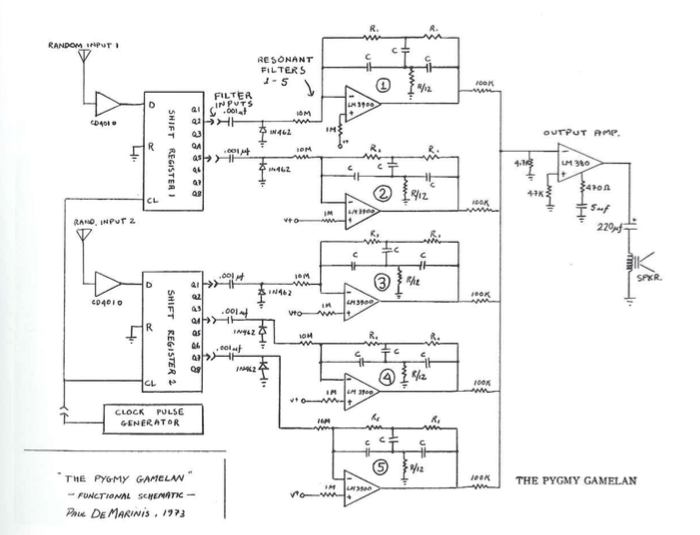
\includegraphics[width=1\textwidth]{pygmyschem}
	 \end{figure}
	 
	 \emph{Pygmy Gamelan}'s importance in our discussion comes from its relative independence from the larger bodies that made it technologically possible \cite[p.27]{beirer2011}. Misuse or re-use of components made for larger consumer devices would prove popular amongst a significant subset of american experimental artists dealing with electronics. 

\subsection{Nic Collins: Handmade Electronic Music} 

Academically, the essence of Tudor’s successors’ would be captured by fellow C.I.E. member Nic Collins. \emph{Handmade Electronic Music} was first published in 2006, presenting an extensive amount of information on homemade electronic instruments with insight from years of experience, references and sources. By completing this project, Collins not only proved that blending academic, commercial and hobbyists attitudes could be successful in all three of those areas, but also linked decades of practices in the do-it-yourself electronic music world to the “maker” movement. The latter started to coalesce around a similar time with publications such as “Make” magazine.

	The values of this book - concepts of imagining, prototyping, assembling from your home - find a strong precedent in pre-industrial craftsmen and the world of boutique electronic music vendors.   \citep{collins2006,ghazala2005,kuivila2004}. 

Although Collins’ introduction hints at the advantages of this approach in the context of electronic music, the advantages of a craft approach to instrument design and fabrication can be further resumed in the potential for personalization, transparency, and skill-transfer \citep{perner2011}. Conversely, the fascination for Collins’ hacking or Ghazala’s more clearly defined circuit-bending can be explained as a desire to fill a need unsatisfied by commercial products \citep{dunne2005}, a process that has shown its ability to serve as the source for entire sub-genres of the musical arts \citep{dunne2005,kelly2009,novak2013}. 
\begin{quote}
“The circuit— whether built from scratch, a customized commercial device, or store-bought and scrutinized to death— became the score.”
\citep{collins2004}
\end{quote}

	Discussing Tudor and Mumma and Kahn, Collins describes the origin of his interest in music hacking, which references the origin of experimental electronics as a legitimate ground for musical composition: 

\begin{quote}
“I learned from Tudor and Mumma that you did not have to have an engineering degree to build transistorized music circuits. David Tudor’s amazing music was based partly on circuits he did not even understand. He liked the sounds they made, and that was enough.” 
- David Berhman \cite[p.ix]{collins2006}  
\end{quote}

\paragraph{the art of hardware hacking}

A look at the structure and content of the work reveals six parts: starting, listening, touching, building, looking, and finishing. Those consist of between two and eight chapters, for a total of 30. Each covers a specific theme such as ``tape heads: playing credit cards'' or ``a little power amplifier: cheap and simple'', revolving around a few schematics, diagrams, guidelines and suggestions for implementations. Historical background is added when appropriate (``David Tudor and Rainforest'', p40; ``Circuit Bending'', p91…). 

There are more pictures than schematics, and what should be striking to anyone already familiar with building electronics is that there rarely are any values or names for parts in schematics - another consequence of Tudor irreverently defacing the key document of electrical engineering. Devising 264 pages of electronics for music involving solely circuits simple enough to describe in a few lines of text appears as a feat in itself. 

	\begin{figure}[h!]
	  \caption{Collins' Light Controlled Mixer circuit}
	  \centering
	    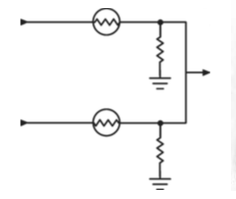
\includegraphics[width=0.3\textwidth]{lightmix}
	\end{figure}

The self-deprecating “keep it stupid” attitude of the introduction rapidly turns into rules number 1 and 2 of hardware hacking, “Fear not!” and “don’t take anything apart that plugs into the wall” (p225). In other words, an electromechanical understanding of electronic music is empowering, and you should experiment as long as you do not risk hurting yourself. This hints at another trope of the open hardware movement, mentioned in the introduction: simple, homemade hardware facilitates sharing and learning, thereby encouraging its practice.

\begin{quote}

“Finally Tim-Berner’s Lee birthed the World Wide Web and a hundred Fuzztones flowered.” 
	
\cite[p211]{collins2006}

\end{quote}

This book can almost serve as an entirely self-contained introduction to electronics in music (falling just short of a soldering iron and a speak \& spell). Collins however made sure that it also is aware of the resources that can compliment it through a list of printed hyperlinks that is fairly exhaustive for its time. In that sense, “Handmade…” also relates to more general current practices in open hardware design. Indeed, it is precisely the open sharing platforms allowed by the world wide web that have fostered the communities which collectively comprise the maker movement. The appendices also reflect loosely broad categories of resources important to both practices: previous documented work. Appendix B appears in retrospect as a paper instructables or hackaday, if every project was hosted on a different homepage. Resources for buying parts and tools are listed in appendix C, where the essentials have not changed and already included allelectronics, jameco, and radioshack. Finally, inspiration: appendix E describes the tracks on CD sold with the book and appendix D lists the rules of hardware hacking and the avant-garde. 
	
	Before discussing the influence of Collins’ book on following publications in related books and articles, it seems important to mention the availability of the book in various digital forms. The original draft for the book, a compilation of class notes, is freely available for download off of the author’s website (w2014). The first result for “handmade electronic music pdf” on most search engines will give a pdf of book.

	By tolerating or passively encouraging open access to resources, Collins contributes directly to the community he has helped shape. More than writing the book on hardware hacking for non-engineers, he’s an essential force in making open hardware design the self-sustaining cycle it aspires to be through the maker movement. By publishing this through a large company while in a professional academic and musical position, he also lends the weight of a more widely recognizable figure to a movement and methodology that challenges the necessity for those very institutions.

\paragraph{impact}  

\begin{quote}

“Collins’s Handmade Electronic Music details many ways in which human interaction can be built into music and sound making devices.” \citep{mills2010}

\end{quote}

	Measuring the influence of this book through simple academic metrics, such as the number of times it is cited in publications following it \citep{harzing2008} yields the following results. “Handmade…” seems to have been referenced in 88 publications (google scholar). For comparison, Road’s “Computer Music Tutorial”, published 10 years earlier, returns 1267 citations, the “Art of Electronics” (a standard circuit design text from 1989) returns 3640, and Gharzala’s “Circuit Bending” from 2005 returns 45. 

	When it is cited, “Handmade…” is rarely commented upon directly. It is referred to in surveys of contemporary sound art, music, and music technology practices \citep{kelly2011,mills2010,pigott2011,rodgers2010}, and as an inspiration in the development of a specific musical controller \citep{ariza2007,hoadley2010,murphy2010,riis2013,valle2011}.
	
	Overall, the academic impact of the work is fairly confined to the field it wished to solidify (music hardware hacking). Its varied content originated from a set of lecture notes, which have since found their place in other college level classes at other institutions. 

On a community level (“do-it-with-others”, diwo, or “do-it-together”, dit), Collins’ impact is difficult to measure objectively. Highly frequented music hardware hacking forums such as Experimentalist Anonymous, diystompboxes, freestompboxes.org, and electro-music.com all contain mention and praises for the accessibility and simplicity of “Handmade…”, but results usually number between 5 and 50. As a reference, searching for Ray Wilson’s popular “music from outer space” do-it-yourself synthesizer website returns between two to three times more results. Collins’ website numbers the quantity of workshops he’s given based on the book since 2004 to “dozens”, meaning that a significant portion of the sharing could still be happening in-person.  

This appears as indicative of the last, and arguably most important point about homemade electronic music instrument design as part of more general arts and crafts \/ diy \/ maker movements. They are fueled by personal engagement and, more importantly, passion. In those circumstances, theorizing, documenting and commercializing is not the priority of the majority but rather the work of the few who turn their passions into a viable working position. 

\section{re-commercializing diy: the maker movement}  

The latest iteration of homemade electronics culture, the maker movement, is described as a third industrial revolution (The Economist, w2014). Here, Fab Labs, modelled after MIT’s NSF-funded center for bits and atoms, allow the public to benefit from some of the efforts of academia to give fabrication a place in everyone’s lives \citep{padfield2014,blikstein2013}. Through this democratization of invention \citep{blikstein2013}, diy culture expands its reach from sunday inventors and engineers to a wider audience. 

In this context, the idea of open source hardware is essential. 

	Often, compelling uses of rapid prototyping (3D printers, cnc mills and other computer assisted manufacturing techniques) are artistic. D-Shape’s large-scale concrete 3D printer is advertised using a sculpture by Andrea Mongante’s Shiro Studio (Shiro Studio w2014). Makerbot’s frontpage for the replicator displays a picture of the device with a completed red plastic bunny on the extrusion platform - this use falls in the artistic range rather than the utilitarian. 

In June 2014, the White House held a maker faire, with president Obama declaring June 18th “National Day of Making” (White House, w2014). Of the 20 projects displayed on the event’s website, 9 were artistic (including 2 instruments: a violin and a banana-synthesizer), and most displayed some level of aesthetic concern. If the third industrial revolution is a democratization of invention, is that the place the arts (and specifically, sound devices) will have? Does a modern version of 9 Evenings exist, and if not, what would it look like? 

On the sidelines of the maker movement, the technology has changed (shifting to digital or mixed-signal systems) along with its means of delivery. Radio Shack and its ilk have lost most of their importance, with online suppliers like Jameco, Digikey and Mouser providing large parts catalogs. Specialized marketplaces like sparkfun and seeedstudio occupy more hobbyist-oriented markets. To compare, by 1970, a Radioshack catalog offered one or two pages , or around .5\% of the catalog for kits, while thirty pages (20\%) are dedicated to parts. In 2002, the last year the company offered catalogs, it contained 25 out of 450 pages of parts, and no kits. The company is currently closing 1100 of its 7000 locations. While this is in no way due solely to the maker movement, Radioshack’s slow death or reconversion does mark the end of an era. 

The rise of accessible embedded systems (arduino, maple boards, raspberry pi, beagleboards…) and availability of relatively free music software (pure data, chuck, csound, supercollider…) leaves music hardware often reduced to the role of place holder for more malleable software. This comes with its own set of design principles (user experience / user interface design), resulting in versatile controllers meant to be used with a computer (monome, linnstrument). With wearable circuits comes the ability to turn most of anything into a controller using the plethora of sensors available to today’s tinkerer. 

Regardless of objective efficiency and versatility, interest in analog sound generation and old-fashioned interfaces is commonplace in electronic music \citep{collins2006}. The range of possibilities for musical expression has become significantly more fragmented. Each approach, whether it is controllerism, hacking or analog traditionalism is being pushed to their extremes. In exchange for this splintering, online resources provide better documentation than before.

The main academic platform for music hardware after 2002 is NIME, which shares all proceedings freely. Amateurs can also find more informal information on a collection of public or semi-private forums (diyaudio, electro-music forum), databases for some type of digital format of designs (hylander), and repositories ran by benevolent individuals that sometimes also try to run small businesses (music from outer space, ken stone).

Most general hardware hacking websites (hackaday, instructables, arduino projects site) contain a significant number of audio hardware projects (hackaday audio, instructables audio, arduino audio forum). It could be said the tools and knowledge necessary for audio hardware designs are more accessible to anyone with an internet connection and the time to teach themselves electronics and programming. In addition, academia is heavily advertising the potential of open source design and manufacturing tools. However, there is very little organized measure or monitoring of the reach of these technologies. Do they truly beneficiate learners and beginners, or do they simply empower some artists and scientists already working on similar projects? Do they only reach people in higher education or with a higher education, or do they attract mostly people already interested in open access technologies? 

The following sections cover two methods of inquiry for these questions. First, recent projects and a series of interviews with their authors allow us to get a snapshot of current practices. Secondly, responses to those projects are devised and documented. An analysis of the process and the efforts undertaken to share those designs follows.

% ---------------
% To incorporate in this chapter
\begin{unsortedStuff}	
\section*{(TO INCORPORATE)}
	\begin{itemize}
		\item 
	\end{itemize}
\end{unsortedStuff}
		
%Blank page to add written thoughts
\begin{optBlankSpace}
	\newpage
	\mbox{}
\end{optBlankSpace}


% ----------------------------------------------------------------------------------------
% CHAPTER TITLE
% ----------------------------------------------------------------------------------------
\chapter{Selected Recent Works}\label{selrecworks}
\lhead{\chaptertitlename\ \thechapter. \emph{Selected Recent Works}}
% ----------------------------------------------------------------------------------------

This chapter describes a selection of designs from the past few years by makers in electronic music. These designs relate in many ways to the concept of open source as it was discussed in the last chapter, that is, devices which in their creation process create some amount of freely available information that enables future developers.

They were selected because they serve as archetypes of a modern vision of electronic music hardware and a related approach to composition. In some cases where the endeavors were purely commercial or secretive in regards to the audio hardware being used, the idea of freely available information still had its importance. Two categories based on their use of a specific technology are identified: CMOS and microcontroller-based devices. 

\section{Devi Ever FX and Dwarfcraft Devices}

Devi Ever FX was initially ran by a Devi Ever, who designed a long list of different distortion pedals before leaving the business to Louise and Ben Hinz. Devi was particularly appreciated in the online pedal DIY scene for her willingness to share and discuss audio circuit designs. 

One of these designs in particular appears as interesting: the \emph{improbability drive}. 

\subsection{the improbability drive}



``http://freestompboxes.org/viewtopic.php?f=7&t=18157&hilit=devi+ever+fx''

\section{CMOS synthesis: modern incarnations}

\begin{quote}
	
	We can make our ``1"-``0" decisions into just about anything- a musical note, a test waveform, a measured and displayed value, a video presentation, a clock, a game, an industrial control, a toy, a microcomputer, an art form, a community information access service, or just about anything else you can dream up. All it takes is the right number of logic blocks properly connected to do the job.
	\citep[pp-7-8]{lancaster1988}
	
\end{quote}

\emph{Handmade Electronic Music} focuses much of its circuits around the Complementary-Silicon-Metal-Oxide (CMOS) family of integrated circuits. He acknowledges inspiration from Lancaster's CMOS cookbook, quoted above (personal conversation, 2015). In doing so, Collins acknowledges how powerful binary signals - an its continuous counterpart, the square wave - can be in relatively simple synthesis environments. Older examples abound: the Weird Sound Generator, a typical first synthesis project sold as a kit by Ray Wilson from the \emph{Music From Outer Space} website, relies on interconnected CMOS chips for its synthesis \citep{wilson2015}. Beavis Audio, an important diy music website, focuses one of its most interesting blog posts on this family of circuits, naming Collins as an influence \citep{beavis2015}. 

Although Collins is not the only source of these digital logic sound generators, the publication of his book has had a visible impact on many of the low-part-count synthesis circuits seen today. The two following examples exhibit particularly interesting and relevant semi-open projects. 

\subsection{Taylan Cihan: Porcupine (2013)}

http://taylancihan.com/porcupine.html

\subsection{Dwarfcraft: the Robot Devil (2012)}

The relative simplicity of the device is here extremely relevant, as it has lead online community members to relate it to some circuits described in Nic Collins' \emph{Handmade Electronic Music}. 

``http://freestompboxes.org/viewtopic.php?f=7&t=18344&hilit=robot+devil''

The power of CMOS logic chips also serves as a segway into the wider topic of microcontroller synthesis. If Tristan Shone's system exhibited the power of arduinos in the context of controllers, numerous practitioners have also been developing instruments  In this case, embedded systems of various complexity have been used in innumerable synthesis projects, providing low fidelity audio outputs and high potential for customization. Sonically, these projects are very much indebted to the auditory product of CMOS chips combined with basic filtering and effects. 

\section{microcomputer systems}

\subsection{Tristan Shone: Author and Punisher}

A mechanical engineer and sculptor, Tristan Shone is the musician responsible for the one-man band \emph{Author and Punisher}. He released a first album in 2005, \emph{The Painted Army} \citep{shone,2005}, as he was developing his first set of instruments, the Drone machines. His website's subtitle is ``electromechanical destruction since 2004'' \citep{shone2004}.

	\begin{figure}[h!]
	  \caption{Shone's live setup around the release of the \emph{Drone Machines} album}
	  \centering
	    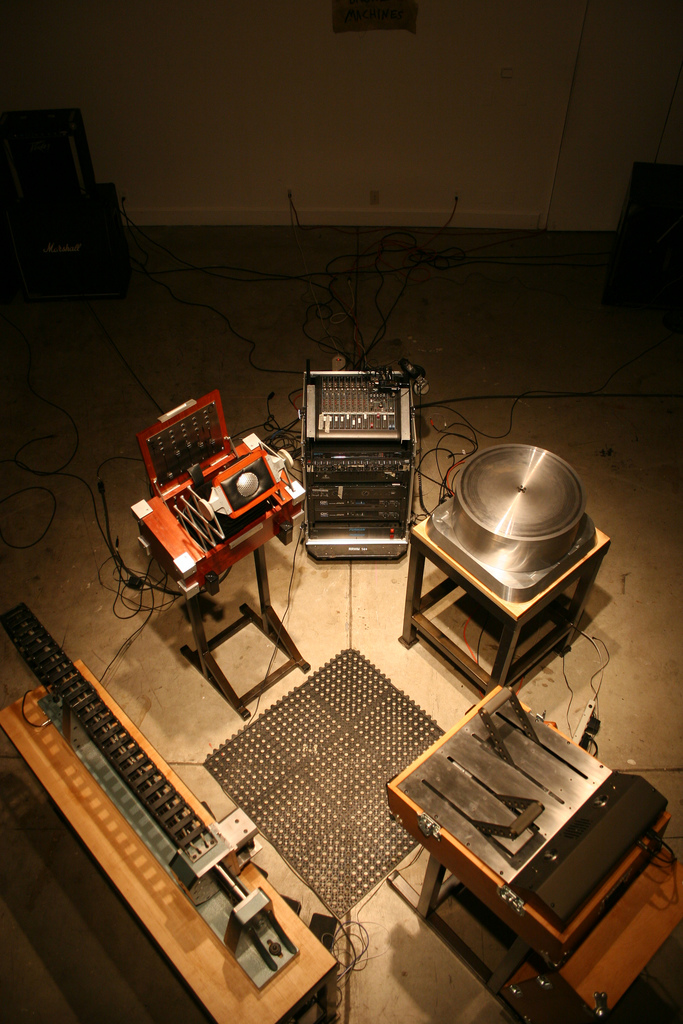
\includegraphics[width=.5\textwidth]{drone}
	\end{figure}
	
He has since released three more full-lengths relying increasingly on hardware he fabricated, in conjunction with a software sampling and synthesis system built around Ableton Live. Most of his devices have evocative names such as \emph{Linear Actuator}, \emph{Big Knobs} or \emph{Bellows}. 

	\begin{figure}[h!]
	  \caption{the \emph{Linear Actuator}}
	  \centering
	    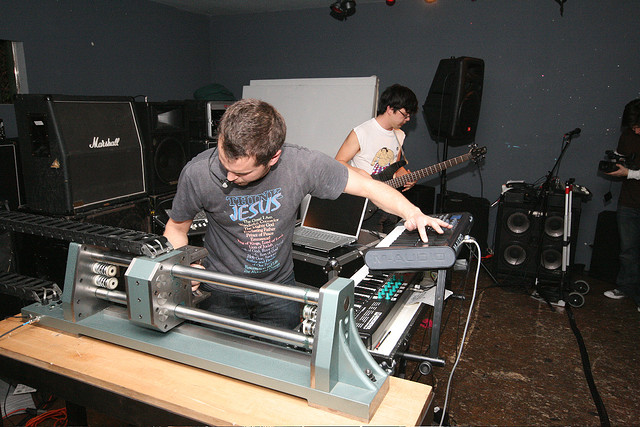
\includegraphics[width=1\textwidth]{linact}
	\end{figure}

	\begin{figure}[h!]
	  \caption{the \emph{Bellows}}
	  \centering
	    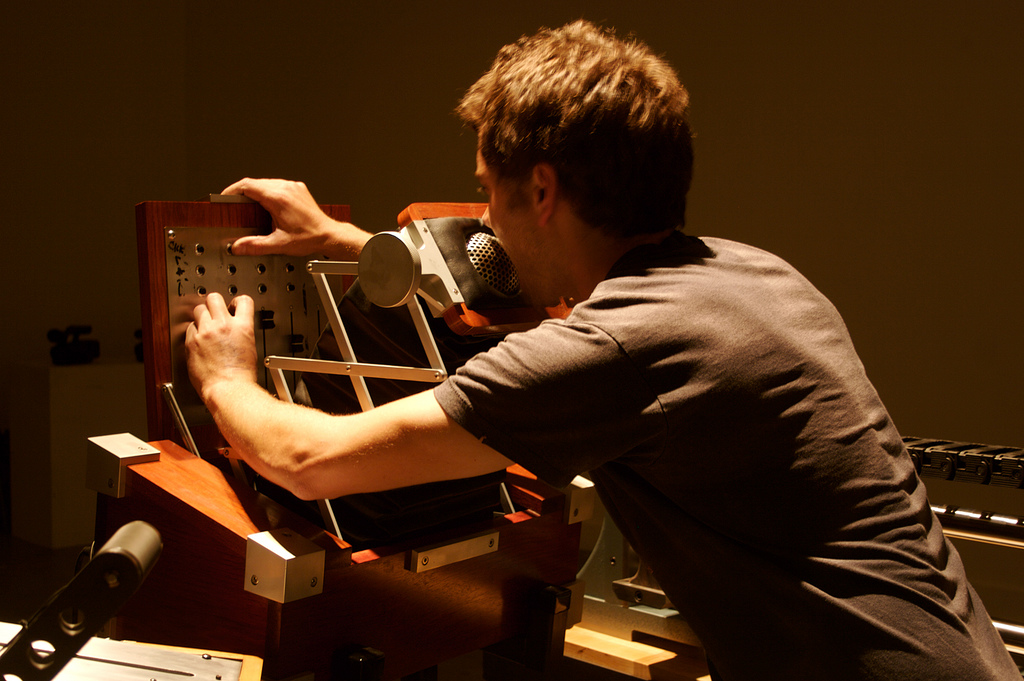
\includegraphics[width=1\textwidth]{bellows}
	\end{figure}

His experience with sculpture and mechanical engineering are clear, although discussing the matter with him makes it clear that he is ultimately making those because they seem like the best way to perform his music. Although he has grown to try and move away from the visual impact of his setup by collaborating with visual artists, his website still provides the curious with a combination of evocative live shots and technical diagrams. 

	\begin{figure}[h!]
	  \caption{a technical diagram for the \emph{Bellows} instrument}
	  \centering
	    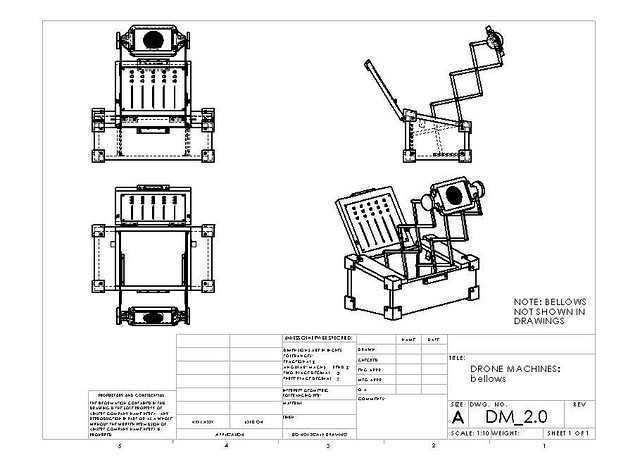
\includegraphics[width=1\textwidth]{bellowsdiag}
	\end{figure}
	
Most of these electromechanical devices act as controllers: they encode movement into a number using a microcontroller. This information is then fed into a computer, which triggers starts, changes and ends for specific sets of pre-composed sounds. 

Shone's microcontroller system is based on the arduino environment, which he uses with custom firmware developed by Dimitri Diakopoulos and featured at NIME in 2011 \citep{diakopoulos2011,diakopoulos2015} . This firmware modification turns a specific strands of the Arduino hardware (the Uno, Due and Mega 2560 boards) into a driverless device, enabling it to send MIDI data over USB without any more setup than a commercial USB-MIDI item. 

However, Shone's live setup is not just centered around controllerism. Shone describes himself as a ``lifelong beatboxer'' and in this context, he's devised a number of ways to detect, record and manipulate his voice \citep{shone2012}. He's currently developing a set of masks (documented on his website are the trachea quad mic, the dither mask, the drone mask and the mute mask), while his previous vocal interface is called the Headgear. That system was the topic of a tutorial written by Shone for the Make Magazine website \citep{shone2012}. 

http://makezine.com/magazine/make-22/seriously-heavy-metal/

\subsection{The Headgear system}

	\begin{figure}[h!]
	  \caption{the Headgear device, wired for operation}
	  \centering
	    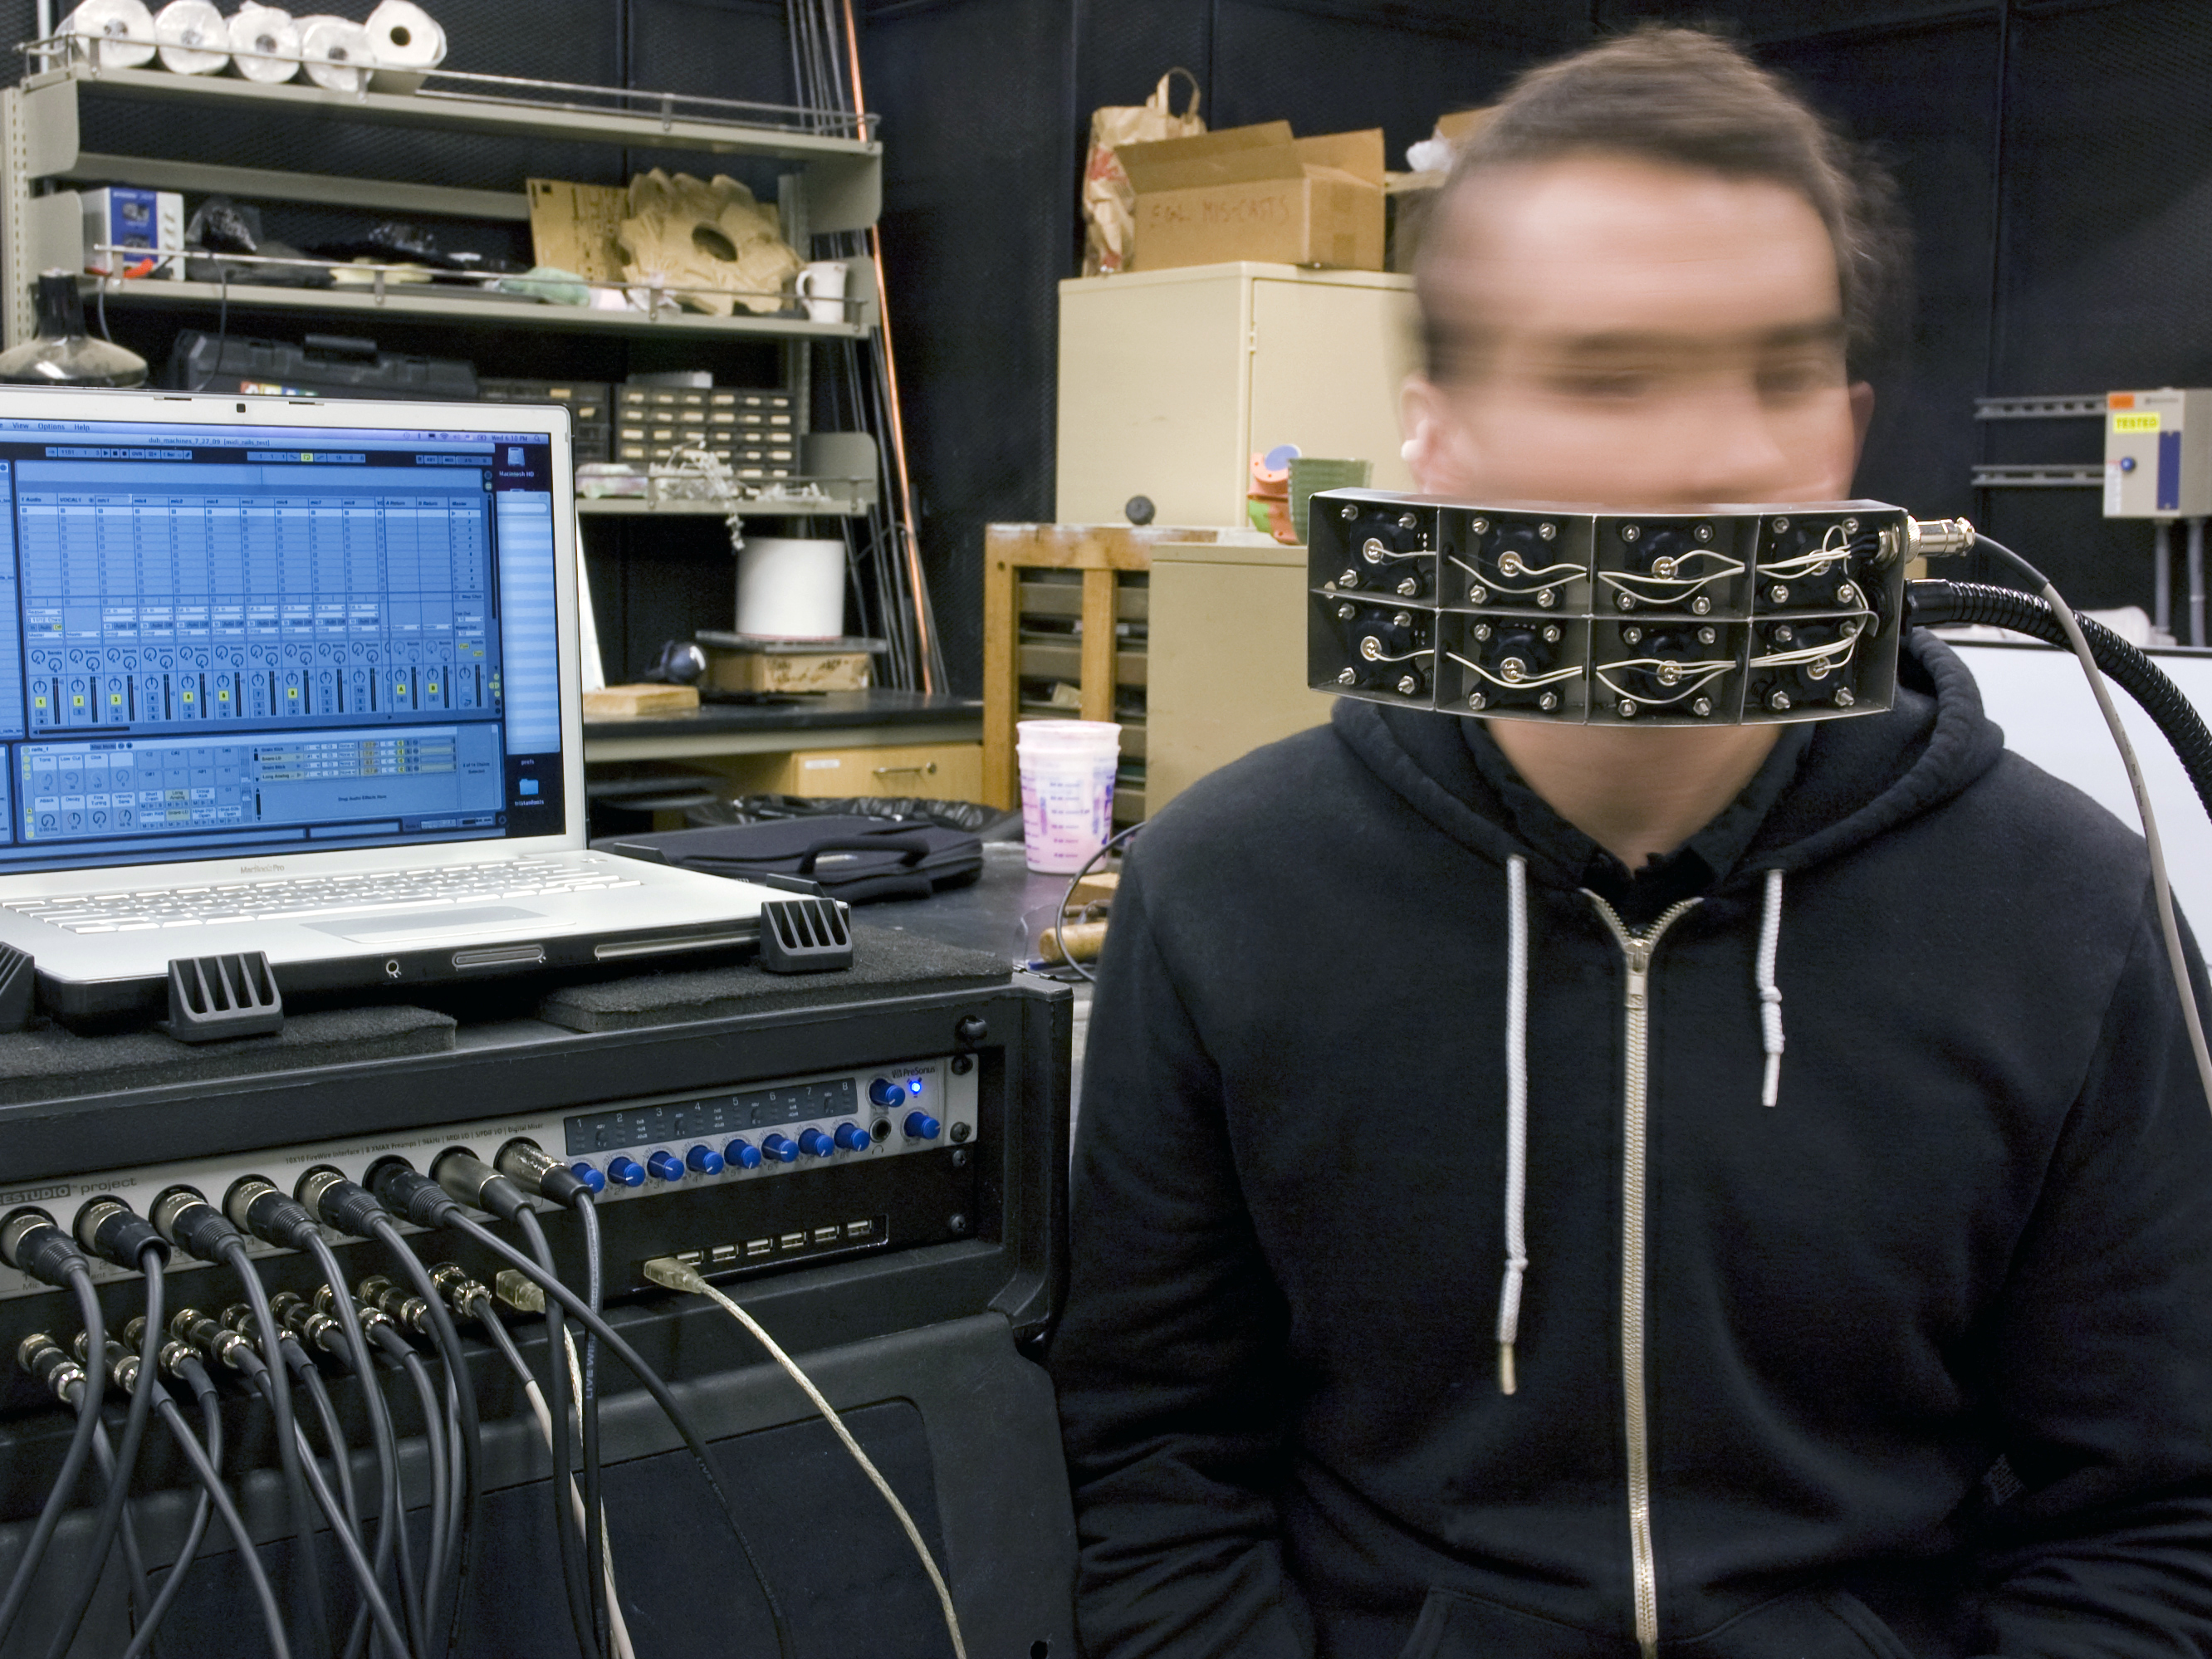
\includegraphics[width=1\textwidth]{headgear}
	\end{figure}

As can be expected in parallel with the rise of microcontrollers as interfaces for turning our environment into a source of control data, recent years have seen a number of initiatives turning accessible, general purpose computing devices into code-based synthesis engines. All these projects are the embodiment of their designer's curiosity, adapted to various degrees of interactivity for performance, composition or commercialisation. 

\subsection{Dan Snazelle, Snazzy FX: the ardcore}

The ardcore is in effect a reprogrammable lo-fidelity oscillator and control voltage generator packaged in a eurorack format and complemented by a set of freely available and editable programs. 

This project was developed by Darwin Grosse and Dan Snazelle. Darwin Grosse is a developper at Cycling `74, while Dan Snazelle is the owner and designer at Snazzy FX. Although the circuit itself isn't publicly available, all the arduino and avr code written by the developers and subsequent public is shared openly. 

https://github.com/eclectics/ardcore

https://github.com/darwingrosse/ArdCore-Code



\subsection{Tristan Perich and Loud Objects}

Tristan Perich's dual approach to music hardware is most clearly divided between his highly predetermined solo work, and the more chaotic performances he presents with Loud Objects. As part of the latter trio, he solders their instrument - a set of microcontrollers - as part of the performance, making the piece a circuit in the most Tudorian sense of the idea. 

As a composer, his work still relies on the binary output of microcontrollers, creating his ``one bit symphonies'' that have been presented as standalone pieces or along acoustic instruments in performances. 

http://vagueterrain.net/journal19/loud-objects/01

\subsection{Martin Howse: the dark interpreters}

Howse's esoteric psychogeophysics exploration is backed by a strong design and programming sense that's allowed him to turn some of his stranger ideas (booting a computer using noise from a metal stake in the ground as some of the BIOS code) into commercial products. 

The dark interpreters is a series of three ARM processor based synthesizer, all available for purchase and with all the documentation for the hardware and the code shared by Howse.  


http://1010.co.uk/manual.pdf

https://github.com/microresearch/dark-interpreter

http://syntone.fr/martin-howse-une-ecologie-des-signaux/

http://www.1010.co.uk/org/darkint.html

http://disnovation.net/bordeaux.html

http://disnovation.net/bordeaux.html

\section{Jessica Rylan, Flower Electronics}

Rylan's circuit design practices present a common dilemna in art-oriented technology today first presented in chapter one: how to make something new and different with the same parts and similar circuits? 

This disatisfaction with the seemingly uniform way modern electronics present audio and think of interfaces is presented as the motivation for a number of designs that wish to address this issue \citep[pp.139-155]{rodgers2010}. 

Inspecting devices sold by her company Flower Electronics over their period of operation (late 2000's to early 2010's) only imprecisely informs one of how this might have been done. Enclosures are still standard Hammond aluminum, and the underlying circuits seem to reference mostly more unusual but known synthesis classics by Buchla, Serge, etc. A clear interest in chaotic oscillators is denoted, but even in that case, it seems difficult to break out of the VCO/VCF/VCA modular mold. 

In some sense, Rylan's work is at its most compelling when it is presented in the context of her own history and musical practice. The personal synthesizer, started in 2004, is the aptly named tool she developed in this quest of alternative design. 

\subsection{the personal synth}

http://vagueterrain.net/journal19/jessica-rylan/01

https://vimeo.com/20051159



\section{Sang Wook ``Sunny'' Nam: Mastering Studio}

Sang Wook Nam is a mastering engineer teaching at Dartmouth College and running a mastering studio at the time of this writing \cite{nam2015}. 

In visiting his studio, it appears that most items in his setup fall within standard categories of equipment: channel selectors, equalizers, amplifiers, high quality analog to digital / digital to analog converters, etc. However, it also becomes clear that all of this equipment is custom made to satisfy Nam's trained and precise ear. In an interesting and probably unintentional nod to David Tudor's mysteriously unlabeled devices, a noted amount of Nam's gear is minimally annotated. 

	\begin{figure}[h!]
	  \caption{Jacob's Well mastering desk}
	  \centering
	    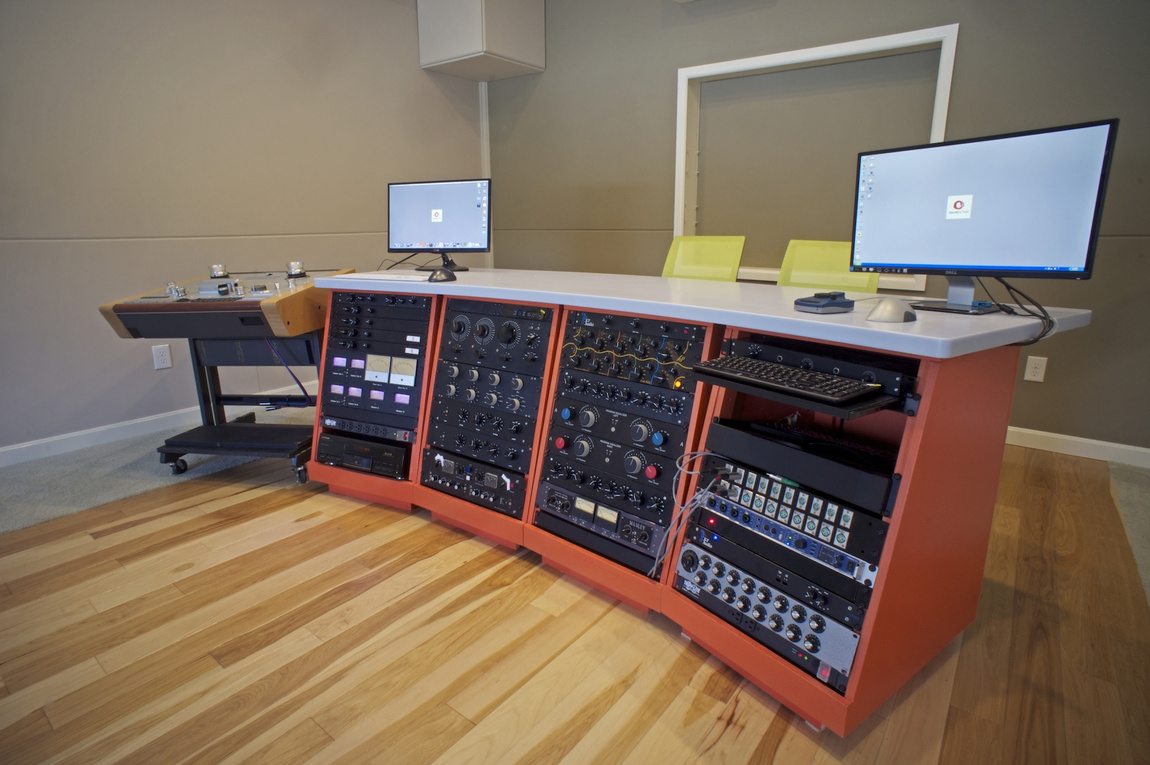
\includegraphics[width=1\textwidth]{sunnystudio}
	\end{figure}
	
Most of this equipment is designed, assembled and tested in collaboration with JCF audio's founder and owner, Joshua Florian \cite{florian2015}. After Nam and Florian worked together at LA's Mastering Lab, Nam came to value Florian's understanding of what they describe as ``yester-tech'' \cite{florian2015b}: older audio hardware circuit designs, usually discrete semiconductor or tube, that were used in high end recording and mastering studios along with the rise and heyday of major labels. A number of parts in Nam's current setup come from A\&R mastering studio, which he purchased when they closed down. 

Therefore, this section does not contain a particular product description. However, this does not mean that Nam's mastering studio has nothing to do with the past and present importance of open source in audio electronics. The very concept of ``yester-tech'' is, perhaps understatedly, at the bottom of the discussion on open-source hardware. Indeed, open-source is mostly defined in opposition to closed-source or proprietary information.

For hardware, this information details the designs of devices, and in most technological economies, this intellectual property is legally protected by copyright, patents. Legally, these expire or have limitations allowing people today to rightfully build and sell their own version of, for example, the API 2520 that Nam mentions in his interview. 

The goals of including comments stemming from my discussion with Nam were simple: prove that secretive designers are still able to succesfully build businesses out of their expertise, expose their use of open-source designs, if any, and that simply taking from publicly available designs was itself a way to perpetuate its importance. In other words, open-source hardware design is a robust practice. 

\section{Design comments}

All these projects are an incredibly limited sample of ideas, yet they appear as varied and interesting in a number of ways. Primary sources range from highly formatted peer review journals to unstable forum posts, mired with dead links and noise.  

%Rather than trying 

% ---------------
% To incorporate in this chapter

\begin{unsortedStuff}	
\section*{(TO INCORPORATE)}
	\begin{itemize}
		\item 
	\end{itemize}
\end{unsortedStuff}
		
%Blank page to add written thoughts
\begin{optBlankSpace}
	\newpage
	\mbox{}
\end{optBlankSpace}



\clearpage
\part{Present: free musical electronics ?}
% ----------------------------------------------------------------------------------------
% CHAPTER TITLE
% ----------------------------------------------------------------------------------------
\chapter{Interviews: highlights and analyses}\label{interviews}
\lhead{\chaptertitlename\ \thechapter. \emph{Interviews}}
% ----------------------------------------------------------------------------------------
\section{Interviews: methodology and highlights}

\subsection{Tristan Shone: Author and Punisher}

\paragraph{highlights}
\paragraph{analysis}

\subsection{Sangwook Sunny Nam}
\paragraph{highlights}
\paragraph{analysis}

\subsection{Louise \& Ben Hinz, Devi Ever FX and Dwarfcraft Devices}
\paragraph{highlights}
\paragraph{analysis}

\subsection{Nic Collins}
\paragraph{highlights}
\paragraph{analysis}

\subsection{Bonnie Jones, Techne}
\paragraph{highlights}
\paragraph{analysis}

\subsection{Jessica Rylan, Flower Electronics}
\paragraph{highlights}
\paragraph{analysis}

\subsection{Martin Howse}
\paragraph{highlights}
\paragraph{analysis}

\subsection{Dan Snazelle, Sanzzy FX}
\paragraph{highlights}
\paragraph{analysis}

\section{Greater context}

\section{trends?}

% ---------------
% To incorporate in this chapter
\begin{unsortedStuff}	
\section*{(TO INCORPORATE)}
	\begin{itemize}
		\item 
	\end{itemize}
\end{unsortedStuff}
		
%Blank page to add written thoughts
\begin{optBlankSpace}
	\newpage
	\mbox{}
\end{optBlankSpace}


% ----------------------------------------------------------------------------------------
% CHAPTER TITLE
% ----------------------------------------------------------------------------------------
\chapter{Expriments}\label{experiments}
\lhead{\chaptertitlename\ \thechapter. \emph{Experiments}}
% ----------------------------------------------------------------------------------------
\section{designing an open source, hybrid and personal framework for signal experimentation: an introduction}

\section{sketches}

\section{drafts}

\section{rehearsals}

\section{results}

\section{to-do}

% ---------------
% To incorporate in this chapter
\begin{unsortedStuff}	
\section*{(TO INCORPORATE)}
	\begin{itemize}
		\item 
	\end{itemize}
\end{unsortedStuff}
		
%Blank page to add written thoughts
\begin{optBlankSpace}
	\newpage
	\mbox{}
\end{optBlankSpace}



% Optional: add gap in contents before conclusion to make it clear it doesnt just belong to last part
\addtocontents{toc}{\protect\addvspace{40pt}}
% ----------------------------------------------------------------------------------------
% Conclusion
% ----------------------------------------------------------------------------------------
\chapter{Future: Conclusion}\label{conclusion}
\lhead{\chaptertitlename\ \thechapter. \emph{Conclusion}}
% ----------------------------------------------------------------------------------------
 
\section{Summary}

In 1950, Lester Paul's radio program explained his peculiar guitar playing sounds with a device, the \emph{Les Paulverizer}. Paul, as a noted enthusiast for innovative uses of technology in music, described this machine as one which could enable him to use ``one guitar, and make it sound like six''. The Les Paulverizer, in reality, was a farce. Its result was fabricated through the use of multiple tape machines and playback speed manipulations ahead of time, then synchronized with Paul's movements on stage. 

Living with the lie of the Paulverizer, its author eventually developed a system that could implement some of its fabled capacities in real time. The \emph{real} Les Paulverizer was in effect a foreshadowing of controllerism - knobs and switches made available to the musician to send controls offstage and trigger various effects\citep{kane2014}. 

Kane makes clear that Paul's style and reputation relied largely on technological innovations such as the Les Paulverizer. Arguably, Paul was succesful in playing with this subterfuge: obfuscation led to commercial and popular success, as well as creative uses of technology. 

Perner-Wilson's third point, \emph{transparency}, has not been much discussed in this work, but is very relevant here: by encouraging everyone to work out the implementation details of a device for themselves, instruments become more transparent.  

%\section{Tutorials}

\section{A note on diversity in audio electronics and this thesis}

This project hoped to address some cultural and social aspects of open hardware design in a musical context: it appears as important to acknowledge the implicit biases present in this process. Most of the people listed here are from the northeastern United States, and arguably all of them have been operating within a western art world. Three of the ten interviewees are women.

\subsection{Geographical Biases}

\subsection{Gender Biases}

\section{Afterword}


Freely shared and discussed technical information in the context of audio electronics was important before the existence of ``open source'' and as such, the tools that have allowed its development have largely been embraced by the musical electronics community. We've seen this embodied in various projects and explicitly expressed by their authors. Arguing the impact of open source, even in its modern sense, could  appear as an redundant task: entire genres are based on experimental, largely unregu


 This debate seems close to ``analog versus digital'', ``tubes versus ICs'' and ``tool versus instrument''. 

The more interesting question has therefore always been to understand the complex technical, cultural and social interplays that characterize the development of new electronic musical instruments. Overall, the ecosystem of invention within which developpers operate offers more background, history and documentation than ever before. Along with that, innovations are presented at breakneck speeds. 

Considering how long the works of Cage, Tudor and Buchla have been capitalized upon, it seems daunting to consider how long it will take for breakthroughs of that caliber to emerge, if ever. However, just like Tudor's work as a composer and circuit designer took the event of his death to really come to a forefront, documentation and responses while these practitioners are working seems crucial. If anything, the only purpose this document wishes to serve is to perpetuate the cycle of information sharing. 



%----------------------------------------------------------------------------------------
%       THESIS CONTENT - APPENDICES
%----------------------------------------------------------------------------------------

%\input{Chapters/sonarch}

\addtocontents{toc}{\vspace{2em}} % Add a gap in the Contents, for aesthetics

\appendix % Cue to tell LaTeX that the following 'chapters' are Appendices

% Include the appendices of the thesis as separate files from the Appendices folder
% Uncomment the lines as you write the Appendices
\part{Appendices}
% Appendix A

\chapter{Interview Transcripts}\label{app:inttrans} % For referencing this appendix elsewhere, use \ref{AppendixA}

\lhead{Appendix A. \emph{Interview Transcripts}} % This is for the header on each page - perhaps a shortened title

These are the full transcripts of the interviews undertaken as part of this thesis. The raw transcripts have been formatted and lightly edited for easier browsing. They are arranged in the order in which replies were received.  

\clearpage 
\section{transcript for interview with Sang Wook Sunny Nam}

The interview was conducted in person in the Digital Musics building at Dartmouth College on October 14th, 2014. 

\textbf{Ezra Teboul}: How did you first get interested in audio technology? What was its part in your learning process as a mastering engineer?

\textbf{Sangwook Nam}: I went to mastering in 2000. There were no resources to learn mastering, but there were books and photos about studios in the US - I was in Korea - and there were tools that known as applicable to mastering. So I used these, mostly digital items like compressors. Plugins were just born by then, so we didn't use them. So we had digital hardware, like waves from swissland (?), and more things from Germany.

After I went to the west coast at the Mastering Lab, they had a completely different concept of the gear they used. I had to learn everything all over again. They're still quite different from regular studios, in those they use mostly off-the-shelf gear. But I had to learn the history of all the recording equipment, because a lot of our designs were based on work from the 60's. I learned how they worked, how they were designed, how to fix and improve them. They're in a smaller form factor now.

\textbf{Ezra Teboul}: Do you hold the distinction between discrete transistor circuits and IC circuits as being important in this context?

\textbf{Sangwook Nam}: Yes - discrete, tubes... transformers, resistors... every part is important. They've all changed, become smaller. The overall quality of the parts and the circuits they're in have been in some sense compromised. I learned how the new technologies, how those smaller form factors damaged the sound of the equipment, and how to keep away from them, all that sort of stuff. What parts I need, how to evaluate them, where to source them...

\textbf{Ezra Teboul}: So you've listened to ceramic vs. tantalum capacitors...

\textbf{Sangwook Nam}: Right. That's easy. But polyester vs polystyrene? What type of polyester? What type of structure? Even with the same structure, what company makes a better polysterene or polyester condenser?

\textbf{Ezra Teboul}: Have you done double blind A-B test for all of those variants?

\textbf{Sangwook Nam}: Yes.

\textbf{Ezra Teboul}: When did you do those tests?

I didn't have any need to do those while working at the mastering lab because my mentor had already done all the listening tests. Wires, switches, volumes, everything. When I left the company, I did it all again myself, because he didn't tell me all of his results. I had seen a few, I knew some of them, but most of them aren't available in the market. In those cases, I had to find old stock from somewhere, and if I didn't find those, I had to find an alternative. So I go on Ebay to look for old parts - from american to russian military to european parts... I went through, bought samples, listened to everything...

\textbf{Ezra Teboul}: I\'ve had to do similar work in the past, and it always seemed like a fun aspect of projects.

\textbf{Sangwook Nam}: It's a fun part, if you're a student. But if you're spending money and time, it becomes more of a problem...

\textbf{Ezra Teboul}: What do you think of your current setup? Is there still work to be done, or are you happy with it?

\textbf{Sangwook Nam}: I'm fairly happy with it. I have some equipment in my mind I'd like to build, still... but my clients are very happy with the outcomes, and I have quite a bit of freedom to do what I need with it, so I'm pretty happy with it.

\textbf{Ezra Teboul}: The fabrication of your custom equipment involves contractors and engineers - most of it isn't built by you. How much do you document this collaborative process?

\textbf{Sangwook Nam}: Well they submit all the schematics and that sort of stuff to me, so I have the final result and a sketch of the design. I also keep all the email correspondence, some notes I take when I evaluate the products...

\textbf{Ezra Teboul}: Do you share any of this documentation?

\textbf{Sangwook Nam}: Oh no. It's a very time and money consuming process. Very good polystyrene condensers cost 200 piece. If I'm testing a stereo pair, I'm spending 400 just for those. Unfortunately, they didn't sound good - so I end up spending 5 to 7 grand just on capacitors. So anybody can do it, but, you know - it's my money and time, and it's really hard for me to share that for free.

\textbf{Ezra Teboul}: Do any of the people you contract for this equipment end up sharing the work they've done through collaborating with you?

\textbf{Sangwook Nam}: The designer and builder of my equipment (Josh Florian - JCF audio) is my close friend, and he's pretty secretive of the information he gets from me. He doesn't use it in his own work or other commissions. Also, its very expensive for mass product, those parts are hard to get...

\textbf{Ezra Teboul}: You've mentioned that learning the equipment was a big part of your education. I'm guessing the other part was training your brain listen to what you want to do, what you need to do with a recording when it comes in your hands. For most projects, what's the technical vs. the mental?

\textbf{Sangwook Nam}: Psychological understanding of what the gear does... will take weeks, months, years. These pieces of equipment I've been using are quite different from modern EQs, compressor... if you've learned how to use commercial standards, you'll have to learn to adapt to mine. I'm using shelf eqs, so I don't have any Q control, any peak curves.

\textbf{Ezra Teboul}: Is it an active circuit?

\textbf{Sangwook Nam}: No, it's all passive. There's only one amplifier at the end. With the parametric EQ most people are used to, it's really easy to go to the frequency you want and take it out, or add something... but you have to be very creative to make something peak- like with a shelf eq. Also the bands are very limited. You need 2 shelf bands to approximate the behavior of one band of parametric EQ, and I have four shelf bands. So I have a very specific strategy to play with the balance of sounds. Also, because those are very wide EQs, you have to get used to that. It's like using nothing but primary colors to paint an image. If you have 48 colors, you just pick up the right one and paint with it, but this is completely different. So I had to learn to adapt my process to these mechanisms, which are very simple but very hard to use for some complex behaviors that more standard equipment can do easily.

\textbf{Ezra Teboul}: Does having a say in the way those items are designed probably helps make it easier for you to use them?

\textbf{Sangwook Nam}: Yes, that's true. Also, certain EQs have some things that they can do better than others. There's two types of filters: LC and RC. LC means you have to use an inductor. If use that, there's a resonance, so you can get a little bit of a peak curve out of it. Also there's the specific sound of the inductor, which will color the output - it might sound a bit more aggressive, or euphonic... so you have to know what this EQ would sound like on a particular sound.

\textbf{Ezra Teboul}: What order filter are you using for your mastering work?

\textbf{Sangwook Nam}: Because it's all passive, I'm using all 6db/octave first order filters. If you want to do 2nd order, you get more parts: more distortion, more non-linearities, more noise. 6dB/oct is more than enough for most cases.

Most EQ slopes in DAWs can get much higher very fast, with 24 or 48 dB per octave being common.

Yes, 24, 48, butterworth... those are common. If I have to do anything that drastic, I can do it in the digital domain, or I can ask for it to be fixed at the mixing stage. If you want to do that at the mastering level, it's a fairly significant problem, so you don't want to do that... That's what's less harmful.

\textbf{Ezra Teboul}: You've worked with Josh as your go to engineer?

\textbf{Sangwook Nam}: He was assistant engineer when he started at the mastering lab. He found at that his interest was in electronics rather than recordings. He's also a great drummer. So he learned a lot from our resident tech back there, what he calls ``yestertech''... tube electronics, discrete, power supply, grounding schemes, all sort of stuff. Then he developed all the new stuff out of that and became the owner of his company that makes great products...

\textbf{Ezra Teboul}: Do you know any other hardware engineers you'd put on the same level?

\textbf{Sangwook Nam}: One of the resident techs went independent thirteen years ago. He's not making any mass-marketed products, but he'll do commissions. His name is Steve Hazleton, in Tennessee. He's another guy that I can go to if Josh is not available. The other people... people who make mass products for consumers had to deal with all the safety issues and regulations that can be problematic for some people. They put a lot of stuff in their designs that ultimately compromise the quality of their work... so I wouldn't call them.

\textbf{Ezra Teboul}: You made it seem like there was a back and forth between you and the designer to get these electronics together, starting with your query for a specific item or modification. Does this process go both ways, and do you listen to some of their recommendations for mastering equipment?

\textbf{Sangwook Nam}: Yes. The equipment that I have... When Josh first listened to what I wanted, the equipment I needed and the topologies I wanted to use, we had to improvise a little bit, which I wanted to do. There's definitely an interplay. He developed a couple of things I didn't think of, and sometimes I'll suggest something he had not considered. That's always going on.

\textbf{Ezra Teboul}: Is there one specific item that illustrates this process well in your studio?

\textbf{Sangwook Nam}: The monitor panel is all custom made. I wanted to listen to what's coming in, and what's coming out. What's coming from the DAW, and compare everything. I told him I wanted those things, so he'll develop a schematic, and explain how each volume is controlled, how to implement mono... how to make those three inputs independent, how to make the panel that has the less contacts. The more connections, the more contacts. Even though we're using very good switches, you'll lose some details. That sort of thing can be more specific points developed by him... ultimately, we decided on three contacts and he built it.

\textbf{Sangwook Nam}: The compressor is another example. I wanted a low pass filter on the side chain so it doesn't see the big bottom end when it compresses it. Since we were using 4 channel switchers, he said we could make it a variable filter, so I decided on four values. 100 Hz, 200 Hz, something else, 400 Hz... That sort of process.

\textbf{Ezra Teboul}: You use only switches and resistor networks, no potentiometers, no faders?

\textbf{Sangwook Nam}: Yes. No faders. Only switches. You can also use relays, or cheaper switches, or any VCA type OPM for switches...

\textbf{Ezra Teboul}: Do you do that?

\textbf{Sangwook Nam}: No, but it's a possibility. But all these alternatives make you lose a lot of low-level detail, so I avoid it. Also the materials of the contact, and their structure... the one I'm using has two contacts. It's military grade silver contacts - gold has a specific sound that's not very useful. So does the copper... Everything has a different sound, and silver is my favorite. It's an expensive switch. It's double sided, so a one pole, twelve out... just one wafer is 60-70... and you have to order thousands of them. The price is just...

\textbf{Sangwook Nam}: Those types of switches were used solely on my console. Volume controls are also only resistive networks.

\textbf{Ezra Teboul}: Do you try to minimize the amount of wiring in the overall studio?

\textbf{Sangwook Nam}: Yes. All hand wired, short. There's still a lot...

\textbf{Ezra Teboul}: Is it all point to point soldering?

\textbf{Sangwook Nam}: Yeah.

\textbf{Ezra Teboul}: So no ceramic boards or circuit boards?

\textbf{Sangwook Nam}: Well, some of the equipment, like EQs... is built with circuit boards. But the console is entirely point to point.

\textbf{Ezra Teboul}: Do you ever take a look at the inside?

\textbf{Sangwook Nam}: Yeah, every three months I'll open it and clean all the contacts.

\textbf{Ezra Teboul}: Do you ever appreciate that wiring as a work of art in itself?

\textbf{Sangwook Nam}: Yes. Fortunately I bought the remnants of A\&M mastering... the founders of that studio were working at the mastering lab and built the console for A\&M studios... So they had all the parts I wanted. And A\&M's philosophy was really similar to the mastering lab's so I was very happy to get that. I had all the good switches, and an already made point to point console. We had to adapt a couple of things, but most of the work was already done. Josh had to do a lot of wiring, but still...

Wiring all those switches... I can't do it. Somehow Josh can do really fast.

\textbf{Ezra Teboul}: Would you ever take out a soldering iron and fix something yourself if it needed it?

\textbf{Sangwook Nam}: No. I'm not good at the smaller things.

\textbf{Ezra Teboul}: How do you know if/when a particular piece of gear is finished? (25min52sec)

\textbf{Sangwook Nam}: We'll discuss the topology. For amplifiers, for example, I usually avoid op-amp designs. Even with discrete op-amp based circuits like the 2520 or 990, those use a lot of feedback, and I don't like the sound of either. So we were talking about discrete amps, like a quad or two push-pulls topology? The shelf EQ has a loss of around 21 dB, so will those circuits have enough gain? He'll build a prototype and we can try it and listen to it. He'll make a test board that has a 21dB loss to test it with, I'll listen to it for a few days, send it back with comments...

After he is done the designs, I listen to for a week or two for anything active. Sometimes he makes a mistake and process stretches a bit, but usually it's just one trip and... done.

At one point, in the very first stage, he sent around 4 different amplifiers with variations for me to try, so I picked my favorite and refined that design. I don't want to overuse one amplifier, because even though they're very transparent, it still has its own sound. I don't want to add the same topology multiple times, otherwise those characteristics compound. So if we need another amplifier, say in the compressor, I'll use a different topology - maybe tubes, or solid state topology.

\textbf{Ezra Teboul}: To what extent do you participate in online audio-enthusiast communities and what role do they play in selecting your equipment, if any?

\textbf{Sangwook Nam}: Human ears can get off-road really quickly. Ears work as comparators. You'll listen to one thing, then another thing, and always compare. If you hear a very bright tune, then a well balanced tune, the balanced one will seem dull. It's very easy to loose objectivity in listening. I had to find a few people that know how to listen to low-levels, to electronics... This is what I usually say: listen to the quality, instead of the quantity. One dB of EQ is the same if you look at the quantity, but every unit has a different sound. People have to pay attention to that, and I haven't found many that do, so I always ask them for a second opinion if I need one. One of them is Bill Schnay, in L.A., and he has a very high resolution recording studio. I listened to capacitors there to pick the ones that sounded the best: we tracked drums in the live room straight into the switch with a very high resolution microphone, and I'll listen to a capacitor with the lowest capacitance to get a sense of what it'll do. He was sitting next to me and helping me, making sure we remained objective. Having a second opinion is really important.

But, online... no. I go there, to find out what the next product is and what people think about it. But the ultimate decision is always with your ear. The people who are lurking... active on those websites... if you're busy, you don't have time to do that. What they're saying is so not true...

\textbf{Ezra Teboul}: Do you measure the performance of your gear electrically, and if yes, what importance do those measurements have?

\textbf{Sangwook Nam}: I do. Good sounding gear has to measure well, but the opposite is not true. Like the 990, it measures well but I don't like the sound. When Jensen first made it, we tried it at the mastering lab, we had a very big live sound at MGM - now it's Sony, back then it was MGM - we put fast instruments like tambourine or any percussion 40 ft. away from the microphone, and rung the bell, or the tambourine. The tails of the sounds decrease, the microphones record that, then we listen to that through high resolution amplifiers that we know with the same gain and it what it does is \"ding\'' then the decay is going on. We can still hear decay all the way down on a good amplifier. The 990 goes \"wiuuuu- ss!...\'' because of the internal feedback. For measurements' sake, you cut out the low level detail, and they think it's noise, and the feedback system cuts it out. But there's still information in that. So measurements isn't a guarantee, but you still need very low distortion measurements to sound good.

\textbf{Ezra Teboul}: Do you look mostly at THD (total harmonic distortion) measurements for this?

\textbf{Sangwook Nam}: The problem with THD and some of those measurements is that they're done using sine waves. What's the easiest thing to measure? Sine waves. What do sine waves have to do with music? Not much. That's another problem of measurement. This can be a good measure of what the amplifier does, but it can't be all of it.
You have favorite topologies of discrete transistor circuits and tube circuits. Do you want to talk about that a bit more?
There's not too much... I like less parts. If I can do with two push pull transistors or tube, I'll use that. If I need more gain, I'll need a stronger design... Tube can be very euphonic, with low distortion, but mostly so at low wattage. Their problem is when they need more power. But if you think about the music, everything is a few watts at most. Drums, or fortissimo would draw a lot of current and require more wattage. But most of the time you're drawing 1, 2, 3, 4 watts. So tubes are great for listening, but not necessarily when you're mixing or mastering those strong transients.
Have you ever considered an hybrid, adaptive amplifier that distributes the load between a single ended vacuum tube amp and a push-pull transistor amp based on the dynamic range of a piece?
I'm not a real designer, so I don't know what that involves. You'd probably need a lot of interfacing between the two sides? I don't know... I have used a tube push-pull amp, and it was really good.

\textbf{Ezra Teboul}: What is most important in your work process?

\textbf{Sangwook Nam}: At the end all that matters is the sound you're getting. It's hard to be objective if you know certain things about your equipment. Forget what it is, listen to what it does and what it can do, where the limits are. It's very bad to have all this technical knowledge without having the listening abilities. I can see a lot of people with that problem, especially on websites. They understand how things work, what's new, but they don't listen.

A funny thing: one guy asked what the best DAW was, and a thousand replies were added on that thread. \"This DAW has this function\", \"that one has another\", but over those thousand replies, no one talked about their sound. That's the current situation of the engineers, and it's really bad. They read the articles and they know the technology... but no listening.

Dither - lots of guys talk about dither. Lots of dithers available. But in my ear, most times dither doesn't work well. For example, if you're using four plugins on one stream, all of those are going to add dithers. If they're using high frequency-boosted dither, even if it's inaudible in one plugin, if you have for or five you can hear that sound and it affects the music. So I tell them to turn of the dither... and they say \"oh no, truncation of errors... no...\". All this information about technology is influencing the way people hear music, and the new technology is always better... In some areas, that might be true, but in music it's not always true. In my opinion, and the history of music says that too, 50-50 is very generous numbers for new technologies. I'd say 20-80. I'd wait 2-3 years after something came out, and trying it in my studio before having an opinion on a particular item. OS, or Pro Tools updates... all sorts of stuff.

\textbf{Ezra Teboul}: In the end, what makes your studio special? You've spent a lot of time listening to everything, and that's why people hire you?

\textbf{Sangwook Nam}: Mastering is special, because in a recording studio you have 48 or so channels to control your quality. If there's a bit of loss in one channel, the consequences aren't always serious. In my studio, my hands are tied to two channels. If I don't use those two channels better than other mastering engineers, I have a big problem to start with.

After that, even if you have a great equalizer, if you play the music wrong, you're doomed. The first thing I can say than my studio can do better than any other studio is play two channels. My DA converter uses a very specific topology different from any other mastering business. It doesn't have any digital filters. You need digital filters to do oversampling - I don't do oversampling in my deck. I don't have digital filters. I have a special process that fixes oversampling and digital filtering that was done during the recording.

So that's the most important part for me. How to play two channels right. In a musical way.

\textbf{Ezra Teboul}: Do you know anyone who has built their own mastering studio from scratch?

\textbf{Sangwook Nam}: All this? Yes, Bernie Grunman. A\&M... which is gone now... the Mastering Lab. So Bernie, Mastering Lab and me would be the three... All the others... I don't know anybody else.

\textbf{Ezra Teboul}: No one who wasn't a professional in the first place is doing this from scratch.

\textbf{Sangwook Nam}: Right. Also, you need to have a tech to build all this, understand the topologies and how to use them.

\textbf{Ezra Teboul}: That's too much for one person?

\textbf{Sangwook Nam}: And too expensive. All the young engineers who build the gear don't have deeper knowledge of yestertech. Everything I see today has remnants of a 2520 or a 990. Some people work with the quad-type amp. But those three represent most of the designs. So it's a pretty limited knowledge base. Now if you have the resources to look for more original things, you have a lot more to work with. The encyclopedia of audio - the first edition, from the 50's. That's the real treasure.

\newpage

\clearpage 
\section{transcript for interview with Nicolas Collins}

The interview was conducted in person at the Native Bean in New York City on February 7th, 2015. 
					
(conversation informally starts on a discussion of headphones, earmuff padding, and the suggestion that the two recordings of the chat will be used with one out of phase to create a composition):
					
\textbf{Nic Collins}: ... In some concert halls, they have devices to jam cell phones. This is known. I’ve seen a handful of references to circuits that do this. this isn’t like building a nuclear centrifuge, anyone should be able to do it. The only tricky thing is working at such high frequencies that cell phones operate at. It’s not as easy as building a fuzztone - the level at which I work.So I see a couple of versions of this, small ones not powerful enough to fill a whole hall, but I love the idea of carrying something the size of an iphone that creates a black hole around, wherever you go, so that in a 3 meter circumference everyone’s cellphone’s stop working.		
					
\textbf{Ezra Teboul}: Have you ever read the Pirate’s Dilemma? It opens with a discussion of the ethical implications of using those ipod radio-emitters for your car. They could jam a frequency not only in your car, but in a 2-3 vehicle radius around you.
					
\textbf{Nic Collins}: There’s so much interest in what’s called s``ilence studies'' in the last ten years. This is cyclical. There’s a Cage / Rauschenberg moment in the 60’s, then it came back with a vengeance... It took so long for Cage’s ideas... not to be accepted, but rather internalized. For example, people from many aesthetics could view silence as a positive element, rather than as the absence of something. It hit something, at the turn of the millennium, when all these people realized you could carve things out of all those negative spaces... and in some fields this had been accepted for a long time. Graphic design... It’s one of those things that follows a zeitgeist or a pattern or a cycle... That idea comes up a lot in hacking. That idea of injecting something or removing something...
					
\textbf{Ezra Teboul}: I’d like to try and go through a few questions, hopefully we can develop that as we go along those. I wanted to start with something basic. I’m interested in contemporary practices in electronic music hardware design, trying to link the first electronic music instruments with diy and Tudorian electronic music and today’s open source movements. You’re in a great position, where you’ve had a chance to work with Tudor but also see taken advantage of contemporary technologies...
					
\textbf{Nic Collins}: I’m old, yes. But I’m still alive.
\textbf{Ezra Teboul}: and you wrote the book!
\textbf{Nic Collins}: fine... I did do that.
\textbf{Ezra Teboul}: So what’s the current place of hardware in what you do today?
					
\textbf{Nic Collins}: ... (pause) you know... because of my age... the arc of my material resources are a little different... from yours, from those of my mentors. I’m from a particular generation. My first work was based on hardware because when I was 17 and wanted to do this there was no computer. It was the epoch of mainframe computers. You would not get access to those as a young person, and even then they were an offline, non real time thing, and from the very beginning I was interested in real time music production and performance. So the alternative was synthesis. This was the era of synthesis. However, synthesizers were also impossible to afford. None of these technologies were what you’d call personal. Ownable.
					
But it was at that moment that integrated circuits went from being extremely functional building blocks, transistors out of which you’d design a whole circuit... to... more modular things, that could do more things out of the box. The most critical chip was a signetics 566, which was an oscillator on a chip. 8 pins, you hook up a very small number of components and you’d get a couple of waveforms. It was designed for touchtone telephones, which is the only reason it existed, because that had a huge market. And across the board, you’ll find people from my generation and a bit older for whom that was the first thing they’ve ever worked with. Because who doesn’t want an oscillator?
					
So... my entry to electronic sound was hardware. But by the end of the 70’s, microcomputers emerged. It was pre-apple, industrial computers. It was sort of like large Arduinos, right? And it was a lot like working with arduinos. So composers from my generation, who are now say between 55 and 70, really dove into the computer stuff early on, and by the mid 80’s it was sort of a no brainer. You could get so much done. The biggest drawback was that you couldn’t really do internal audio processing on a personal computer until the 90’s. But there was so much available in terms of MIDI controllers and everything, and I basically since 1979
					
kept two parallel tracks of doing these circuit based things and computer based things, because the fact of the matter was I wasn’t terribly interested in the sounds of synthesizers... so I had to find other roots.
					
\textbf{Ezra Teboul}: and a summary of that is in your paper about early microcomputers in your practice?
					
\textbf{Nic Collins}: Yes - that’s the paper on Semiconducting (see http://www.nicolascollins.com/texts/semiconducting.pdf). It’s the idea that certain technologies have natural strengths. from my standpoint. And most composers think of orchestration as a decision, rather, than say writing for violas the rest of your life. So for me, switching back and forth between technologies was no different from switching back and forth between instruments.
					
But I have to say, as the decades passed, it was obvious that the computer was becoming the more powerful, more versatile tool, and if I wasn’t willing to spend the time being a brilliant analog engineer - I was always self taught - there was much more possibility and much more openness and much more of a community for a sort of open source in the software domain, rather than the hardware domain. But I kept a hand in the hardware all throughout this time. If you look at the few records I’ve done over time, there’s all these oddball instruments. Hybrids of electric and mechanical things. Sometimes maybe guitars, live sampling systems... It was all a mishmosh. What happened, what changed for me was that the end of the 90’s, I started teaching in art school. It was this moment where you may be able to identify more clearly... I call it the digital hangover. The computer had become so powerful that people were just knocking back shots without think- ing of the consequences. You couldn’t really do anything. My mantra has always been control-x / control-v. It’s the world’s most powerful tool! You can cut a term paper, you can cut audio, you can cut video, you can design a website. It’s the world’s most amazing pencil. But as I discovered, from the art school context,
				
					
art students are peculiar in the sense that every single one of them, even if now they do exclusively digital, they all started drawing. There is not an artist in the world that didn’t scribble, even if now they use a mouse. And that seems to be really ingrained in visual artists, this desire to do things with their hands. We think of that as a musician’s thing - musicians are about the tactile. But I think that musicians don’t play their instruments 24 hours a day. They have a nice life+work separation. Artists are always fiddling with something.
					
It was those students who pushed me to do the class, and it was this generation of hungover... from digital overindulgence... that led to the rise of Circuit Bending. Because the Circuit Bending movement went back to the early 90’s, when Reed Ghazala star- ted writing articles for the Experimental Musical Instruments journal (EMI: see http://windworld.com/features/back-issues/) . And there was always a little cult of this stop. Always this buzz in the air about the Speak & Spell. I had a Speak & Spell in 1979 that I hacked. this is pretty basic stuff. But he took off at the end of the 90’s, with this sort of anti-computer backlash. For a while people were waking up one morning and saying oh``I’m never programming again''. And for a while it was like that, a real split between the circuit bending people and the computer music people, and they basically had nothing to do with each other. Circuit Bending people were militant about their anti-computer stance. Porta-studios came back with a vengeance, the cassette was a real format... It was almost like a luddism. But then... a few things happened. The most important one was the sort of parallel growth of limits in the open source community and the Arduino.   People had been making arduino type things since the 80’s... STEIM made this beautiful sensorlab thing - but it was \$3000! Completely insane. So the combination of the affordability of the Arduino and the open source nature of doing programs on it and the fact that they had provided this glue between the physical world and your laptop meant that it was like the peace accord in Belfast.
				

Suddenly catholics and protestants could talk to each other - over the top, but I
					
think a lot of orthodoxy broke down at that point.
					
\textbf{Ezra Teboul}: people realized the Speak & Spell used microcontrollers.
					
\textbf{Nic Collins}: That’s what I tried to tell these guys. Every single toy they use is a sample- playback computer. I did a workshop with the other Nick Collins, in Mexico, some years back. There was so much confusion about the two of us. He’s a Supercollider maven, and the organizers could not figure out these two dudes were two different people, so they billed these multiple workshops with Nic(k) Collins, with no indication of which was which - there were 2 or 3 of them. And of course everyone came to all of them and they didn’t know what they were going to get. We decided we would simply do the workshop together and every hour we’d switch between software and hardware. It worked! It was clearly the threshold point. Everyone was equally comfortable working in the two modes, which was a big change. Where does that gets us?
					
It gets us where we are today. Coming into teaching late I’m much better at making the distinction between my life and my job than I was when I was a grad student. But I can’t deny that teaching, not only in Chicago but also these countless workshops have fed back into my own practice. I got interested in one very specific thing at the beginning which is that when I would do a workshop I would have 25 kids sitting around a table with little amps and speakers working on kind of similar projects or technologies at the same time. Everyone would be working with contact microphones, or making their first oscillator. But it was this great orchestral electronic sound, that wasn’t mixed down to a P.A.... it’s also in the same general region, but uncoordinated. Now for a guy who’s background is in deep Minimalism... I started opening up to a chaos... the things you can get with a large number of human beings that you can’t get with a line of code - unless
					
you’re really really clever - and I’m not, I write relatively simplistic code. So I got interested in the group dynamics of hardware based stuff, where you don’t control things as accurately as... god forbid, a guitar, in your hand. 25 electric guitars in a room, it’d be a very different experience. I got interested in the noise world. The sound world of... disreputable electronics. Electronics that you weren’t sure were working correctly, or that you knew was damaged but still interested in the sounds it could make.  So I did a piece called ``Salvage'' - it’s on youtube – where six people try to revive a dysfunctional or broken circuit by injecting voltages into an unpowered circuit board and using it as timing components for oscillators. So you get a very complex oscillator with a high degree of chaos in it. And it goes through a set of complex evolutions as more people start joining. There’s a very simple instruction set. The idea is that it starts out relatively cause and effect-y, because there’s only one person doing this, but by the time you get up to 6 you get this sort of density of decision making that’s very difficult to think about being done with a computer.
					
That being said, you know George Lewis made these really beautiful programs that improvise. George has been working since about 1980 on program that improvise. And because he is such a great improviser, he’s someone you should pay attention to. The basic idea’s always been that the computer listens to the player, and responds as if it is a player. The reason I mention this is because instead of creating a standard algorithm for what its improvisation should be…. (to the best of my knowledge, and you’ll have to confirm this with him, what he’s actually done) is that he’s written different routines that embody different improvisers that he knows. So that in his computer he has multiple different personalities that behave differently in response to the same data.
					
Now if I was smarter I would try to do something like that. Computer program that instead of having 6 people doing something I have one person do it, and then five ``people'' to play along. At the same time, I always have a lot of warm bodies in this workshop and this one way to harness the energy. I’ve spawned a couple of solo pieces of from that. What I’m trying to do is harness the apparent chaos and conformability - seemingly incompatible - of some analog circuits - but use software as a way to get rid of the the sort of monophonic property that most circuit performances have. To create some sort of complementary behavior.
					
Do you want a précis? A short version? I’ve carried parallel practices in hardware and software for years and years and years. They’ve always worked together but what I would say is at the moment, it’s the chaotic aspects, the instability of circuits that are coming to a full forward in the stuff I’m doing.
					
\textbf{Ezra Teboul}: So has there been any one device or project that has created a noticeable shift in your work?
					
\textbf{Nic Collins}: No, I think there’ve been multiple ones. David Tudor used to talk about how he never understood tubes, and then Gordon Mumma tried to teach him how tubes worked, and they tried to build a tube amplifier, and tried three times, finally giving up. It wasn’t until the transistor came around that he was comfortable making circuits.
					
For others of us it was the integrate circuits. I’m lousy with transistors, but ICs are a piece of cake. The more complete building blocks are great. My whole book is predicated on this CMOS logic circuitry (26:18) from the 70’s that lent itself beautifully to running on batteries. That was a critical technological bridge.
					
For most people, it was the advent of midi and pc with reasonable userbase, so that
					
software could be made by people other than yourself. In the 80’s, the conflation 
between the music industry and the computer industry was critical for a lot of people. It didn’t matter so much for me, a lot of my stuff had backed off from the computer, but for the community at large...
					
Then when computers actually got fast enough to do real time audio processing. So when Max went from being a MIDI generator language to control synthesizers to having an MSP component that allowed you to do direct sound manipulation, that was a big deal.
					
And I think... I don’t do a lot of stuff with Arduino at the moment, but I know that that has been the next big step, because it’s solved the problem of connecting the computer world to the physical world. Foundations like STEIM had been working since the mid 80’s to make that work, spending billions of dollars on artists residencies and research. And suddenly, this Olivetti guy shows up and \$25 later, you got it all worked out. So you know, open source and Arduino would have been the next big step. And I suspect that this is going to be very important. One of the guys who started the first laptop orchestra at Princeton is now doing an iPhone orchestra at Stanford. Ge Wang and Perry Cook... they had a very conspicuous laptop orchestra, and when Ge gets out to Stanford, he ups the ante and starts a phone orchestra.
					
\textbf{Ezra Teboul}: Dan Iglesias made a nice wrapper for LibPD called mobmuplat...
					
\textbf{Nic Collins}: Oh right, that’s why the name is familiar. It makes a lot of sense, there’s still a lot of people who don’t want to use their computer on stage. They just like the idea of wrapping it up in a smaller package. A point was made to me that people are developing apps much faster than people are developing full feature software for larger platforms. For every major rev of Ableton or Max you have a million new apps that allow you to test all these areas of work.
					
\textbf{Ezra Teboul}: Is there anything you’re curious to see implemented? 
					
\textbf{Nic Collins}: I would be interested in - and I think some people have done this - but I’m very interested in sort of the electromagnetic spectrum that we have around us. Christina Kubisch does these really beautiful EM sound walks, and I do all these things with coils in my workshops where you pick up the sound of your iphone... but I’ve always been curious what the wifi traffic sounds like. Make a really simple receiver in that bandwidth, with a frequency shift to bring it all down - not to steal the information, I couldn’t care less what people are doing - but to hear if there’s any rhythmic quality to the community that’s working in that spirit.
					
\textbf{Ezra Teboul}: there’s somewhat of a visual equivalent that’s been done, with some code sniffing all the image content being downloaded for people’s web pages and attempting to recreate an approximate mosaic of the overall network’s image consumption.
					
\textbf{Nic Collins}: and I’ve seen demonstrations of some of these slightly suspect softwares that allow you to look at wifi traffic on a network. clearly it can be done. It’s just that there’s some difference between extracting the data, and my desire is so much simpler - what is the sound of all those things going back? You do have to do a little of stuff, because even when there’s no data there’s still a constant carrier, so you have to get rid of the droniness...
					
It’s an interesting point. There’s this  essay called ``Yes We Can. But Should We?'' (https://medium.com/re-form/just-because-you-can-doesnt-mean-you-should-252fdbcf76c8 ), and it’s a reaction against the diy community. There’s just a sense that its creating so many things? do you need to be making all these things? The downside of this world you’re looking at is it leads to a prepon- derance of things. It has environmental impacts. Recycling software is much better than throwing out a circuit with a battery in it. It’s a question of resources. Then there’s the moral aspect, the psychological aspect of hoarding, with being object-oriented. If you’ve talked to people in bending communities, very often
									
the instrument remain in the forefront of musical practices. There’s something pretty dreary about concerts at Circuit Bending festivals. It often seems like the music might be an afterthought. There’s nothing wrong with being a luthier. There are people whose tradition is building great instruments. It can be Stradivarius, it can be Trimpin, it can be the engineers that are behind the cracklebox, it can be bob moog, but they’re not necessarily the people to whom you want to listen to records by. So I think that there is a need to be clear about that. From Tudor’s generation down, there’s an air of tension. Am I going to be taken seriously as a composer, if I make this thing? Am I going to be taken for an artisan?
					
\textbf{Ezra Teboul}: That’s one of the things that’s fascinating to me about Tudor. He comes from this very respected musical standpoint, but embraces the experimental electron- ics, live electronics practice, and he’s taken very seriously. But that seems to be mostly because of where he’s coming from. Not necessarily because people objectively thought his electronics were producing compelling compositions...
					
\textbf{Nic Collins}: It’s complicated. He had this reputation as a virtuoso pianist, and then the artistry was elevated in his role as the interpreter, the realizer of these Cage pieces, whose scores had to essentially be translated for performance. That act of conversion, he elevated to this high art, which very few people have reached since. After that came the creation of these electronic instruments in service of the cage scores, and after that came David Tudor as composer. It was too many talents that leached stuff along the line... there was a smaller vocabulary left to describe it, so to speak. I’m very conscious - I’ve known the guy from the early rainforest period - I’m very conscious of the fact that it’s only after his death that the composer aspect of him began to be treated seriously, in terms of the the written stuff... There’s that issue of the Leonardo Music Journal called ``Composers Inside Electronics'' (http://leonardo.info/isast/journal/toclmj14.html), which coincided with a symposium marking the donation of his archive to the Getty in LA. That’s where you’ll see a nice overview of the different periods...
ET:Do you know about the Little Bits kits?
\textbf{Nic Collins}: Yes 
\textbf{Ezra Teboul}: Korg has a series of synthesizer based ones...
					
\textbf{Nic Collins}: I’ve seen a number of those things developed over the years... Radio Shack even tried a few times to make some of those lego-y things to teach electronics. Since my kids were really into lego, I tried to show them that, the mindstorm things too... But my kids never latched on to that, and I never invested much time into using these for artistic experimentation... I think it’s all quite good - here’s my take, getting back to this idea of because you can do it, should you - we all tend to loathe ourselves and the group we represent, so I’m always very conscious about promoting ourselves and the ideas... I have this weird reputation as the hardware guy. If you read about me 15 years, I’d have this weird reputation as the computer guy. These things change. But am I weary of people setting camps.``I’m not going to use unless I make it myself'' or``I’m not going to use it unless it’s linux'' or that kind of statement... but I do think that one of the great virtues of learning to program or learning to work with hardware is that we get a better understanding of the technologies that our lives are ruled by, across all domains. My father’s generation was one that tinkered. He was a college professor, for christ’s sake. He’d build a bookshelf, not go to ikea - we didn’t have ikea back then. If the car fucked up, he’d try to fix, whether or not he actually could. It was assumed you would open the hood and check the oil, and make sure the cables weren’t frayed, and you’ try to second guess your mechanic.
					
I tell people how the first time I was in Europe in the mid 70’s, I was in Germany and I saw that all the driving schools has these models of cars, cutaway models of car with this cross-section of the transmission and everything! Like the visible
									
fish. I learned later that to get a driver’s license in Germany at that time, you had to answer questions on the written test about how a car works. Not just what this sign means, but also explain how a carburetor works...
					
\textbf{Ezra Teboul}: which is what HAM radio tests are today...
					
\textbf{Nic Collins}: True. Trevor Pinch edited a really nice companion to sound studies (http://www.amazon.com/Oxford-Handbook-Sound-Studies-Handbooks-ebook/dp/B00BQES54M/ref=sr_1_1?s=books&ie=8&qid=1427399248&sr=1-1&keywords=oxford+handbook+of+sound+studies). It includes a really beautiful essay on German... in germany in the 30’s, there was this emphasis on diagnostic listening. You would be taught to listen to the engine of the car to pinpoint defects. My father’s generation, they’d be taught to replace the tap washer when it would drip. The idea was that the technology was open. Even if you didn’t understand what was happening, people would open the hood. People do not open the hood anymore. One of the things that happens in my workshops that is ultimately the best takeaway, is that there’s always someone that comes up and mentions that dreadful word, ``empowering''. They may never touch a circuit again, they may have done this because they thought it’d be fun, or because their boyfriend was doing it or something like that, but they say it was the first time ever opening a radio or this or that. It’s the first time they’d ever touch their part.
					
\textbf{Ezra Teboul}: Do you feel like there’s more than intuitive connections between this long- standing practice of opening things up for music and the more recent open-source movement?
					
\textbf{Nic Collins}: I think it’s very unlikely that an obscure music fringe had an influence... I do think that there are certain social trends or zeitgeist that have a long nose, rather than a long tail. A long nose, where you sort or see these signs of a build up. Take something like the arduino, which has a very strong presence in the diy community now - it’s a very good universal tool. As I say, you can look at proto-arduinos that have been produced since the late 80s, but it had to hit a
									
certain price point. Just like circuit bending took off because there was a shift in cultural consciousness, there was a broader acceptance that you didn’t need to know what you’re doing. My generation, even though we were terrible engineers, we really tried to understand what we were doing. The only reason we would do something interesting is because we didn’t [understand what we were doing], but we tried really hard. When the benders came around, the whole idea was ``don’t tell me how this work''. I have this quote in my book, one of the first things that happened: I was setting up on a little table for one of the workshops and this mountain man comes up and asks ``are these bent or hacked?'' So I ask him what the difference is and he says ``oh, um, bending means you have no idea what you’re doing when you open it up, and hacking means you have a little bit of an idea.'' Then I thought, from an ecclesiastical standpoint, that’s kind of interesting. So we had that ground shift, and it was the same thing with programming. I remember when we first started with microcontrollers it was like ``this is going to be hard, we have to learn how to do this, we have to learn how to do that''. And my students discovered that no, all you have to say is I want to control the speed of a motor, all you have to do is search motor speed control arduino, you get a chunk of code, you cut and paste. So that is amazing.
					
I think there is still an issue, which could potentially be called a problem, which is what we might call the preset idea. When the DX7 came out, it had such an amazing timbral palette, compared to most other things. 98\% of the users never got beyond the presets on the front panel. There were many, and they were very rich. Except they were finite in number, and after a while you could pick them out in pop songs. The algorithm for FM synthesis has a certain sound to it, but some people did remarkable stuff to it, really differentiated it from the presets on the front panel. The problem with bending is that in a way it’s a bit like presets. In other words, we are now on the speak and spell preset or the casio preset - and you can identify them. With the cut and paste approach to code, it can lead to something similar, which is that module of code, which you didn’t end up tweaking very much because it did a good job... now something like motor speed control is pretty utilitarian, but there are other aspects. But you look at other languages, Supercollider, Max MSP - those are very open as to what they can do. But both languages, Max in particular, come with all these modules, these objects, that are very powerful but also quite recognizable. There was a period of several years where I could identify a max patch just by hearing it. It mostly had to with the sample playback stuff that Max did very easily. It was another boon to people who were starting out, but it was a sort of presetting.
					
So this is potentially a danger with the app market. It takes a very powerful programming environment, and it generates one patch, so to speak. If you develop it yourself, you’ll spend some time tweaking this and that, then you can use it in 3 or 4 different pieces and it’s adapted. When its an app, it sort of sits there begging you to use it and have it be your instrument.
					
\textbf{Ezra Teboul}: For me there’s sort of two origins for presets: the community at large, the programmers - those are the tutorials, example patches that are built in and the cycling 74 website - then there’s the patch your friend made next to you. I think the distinction is important and interesting, for how those two communities work together. How do both communities influence your work? How important have other people been in the development of your work.
					
\textbf{Nic Collins}: It’s a mix. Statistically, the students of the workshops have been more influential than known individuals. With one or two exceptions. In the early days of the workshop, I had this vocabulary of techniques that were chosen because they were relatively easy to do, inexpensive, and most importantly they did things that computers couldn’t do easily. I wasn’t trying to do stuff... I was trying to match
						
a market need. It wasn’t a Moog synthesizer and it wasn’t a computer. Along the way, the assortment of project and the tweaking and tuning of them was very much influenced by the feedback I’d get from people. The other thing is, people suggested stuff. There was this guy, John Bowers. A computer science professor, and he’s also done really interesting low end electronic stuff. He was the one who showed me this business of the making a speaker into an oscillator with just a battery. He called it the victorian synthesizer. He brought it up when we were doing a workshop on loudspeakers and all the things you could do with them. Now this is a standard part of the workshop I do - it teaches you so many things, you can get it going instantly... But I look around and... I sort of see what people are doing. It feeds back in. But my general instinct is that I get more from general feedback from the participants.
					
\textbf{Ezra Teboul}: so this is the side of the community that you feel is more influential than your peers?
					
\textbf{Nic Collins}: yeah... maybe just because there’s so many more of them... maybe it’s because they’re younger, and they have a keener insight into what’s changing. I’m always looking for the next thing. Starting about 5 years ago, I saw this interesting, incredibly low level electronics. I see this sort of arc, which is best represented in Korea. There’s an awesome scene in Seoul. It’s Dotolim and Balloon & Needle project. Otomo Yoshihide comes to Seoul, and it’s like this catalyst for this sort of noise. And you see this evolution: lets start a band, then lets add the effects, then it gets noisier and noisier, and then they say lets disconnect the instruments and use only the effects. You go from Otomo to Japan Noise... then you get to the point where they say lets open up the effects, lets see what’s inside, lets do a piece with just the one transistor we pulled out (56:37) from the pedal... let’s just do something with dirty contacts. It’s this funny kind of arc that’s represented
very well in the Korean scene. I’ve seen this post- effect pedal stuff happen. It’s
					
really interesting.
					
\textbf{Ezra Teboul}: How do approach limitations in your work? Have proprietary tools and designs or planned obsolescence affected you?
					
\textbf{Nic Collins}: The notion that if you pick up an object, whether its a violin or a chip, it has certain limitations built in to it, that would impose a method for using them?
					
\textbf{Ezra Teboul}: Throwing back to the notion of presets we were discussing earlier.
					
\textbf{Nic Collins}: That might be why, as I say... I for one try to avoid defining myself by a medium... like computer music or hardware hacking or chamber music or improvisation. I’m sure there are people who are happy being in such a niche. I like string quartets or I like piano music or I write for Jazz bands... But my personal interest is to seek out different resources and work within the confine of those. If you look at my background, there he was with Lucier, sort of experimental music, electronic scene in the 70’s, then in NY in the 80’s, working with improvisers and downtown bands, then in Europe in the 90’s, working with chamber ensembles, now in Chicago, in the boondocks, teaching at an arts school, and he’s created this whole cult of workshop based hardware practice. Each one of those has provided its own benefits and limitations. But I think that’s something that’s ubiquitous to art practice. I don’t think it has to do with a time... it’s always been the case. I’m only saying this because in art school I’m very conscious of the fact that these days you have very few students who define themselves in terms of medium. Few people say ``I’m a video artist''``I’m a sculptor''... they say``I’m an artist''. And then oh``h yeah I also do some video and some other stuff and I draw and I’ve done a print edition''. The only people that define themselves by medium these days are painters. Painters still do that. And not all of them, but that’s where you get the
highest concentration of self-identified students within a medium. Next question!
					
\textbf{Ezra Teboul}: Is personalization of electronic music instruments just a set of decisions con- cerning which limitations are acceptable?
					
\textbf{Nic Collins}: Yeah... I think people sometimes have different ways of defining what’s an instrument. But from the classical era to the the rock and roll era people said ``I’m a violinist'' or ``I’m a pianist''. The conductor was the oddball, but people who made music defined themselves in terms of their instruments. What happens is now, post-electric guitar, the instrument has expanded. Is an electric guitar just a string and a neck? or does it have an amp ? How do you relate to the amp? Oh, you use a pedal. Is it a fuzz, and overdrive? Suddenly you’re performing in this network of technologies. Then as I said with my Korean friends you disconnect the guitar, you only play the pedals... there’s the transition. I think that it’s more difficult now to localize yourself as an instrumentalist. Then you fall into this thing of realizing that an electric guitar is an incredibly versatile instrument. It’s been used in so many styles of music. Nobody ever says ``oh my god not another electric guitar''... well they do, but not in the same way they say ``oh, a wah-wah pedal...?'' or ``a vocoder?''. If you call yourself a wah-wah pedal-er, it seems... much more limited. And maybe it’s that preset thing again. It’s got such a limited range, it doesn’t cross that threshold of expressiveness. That being said you have people that have made a point of working within that. People like Toshi Nakamura and the no input mixing scene. Some of that is incredibly limited... or Sachiko M’s early stuff with samplers, where she only played with sine waves, the test tone in her sampler.
					
\textbf{Ezra Teboul}: Hannah Perner Wilson’s MIT master’s thesis discussed making basic components from scratch. She defines the advantages of such a practice as the opportunity for personalization, a better chance for transparency, and the importance of skill transfer. Any thoughts on this?
					
\textbf{Nic Collins}: I’m doing an advance hacking course this year, so I’m in that right now. We’re doing sophisticated designs, but also stuff like baking our own piezoelectric crystals, so we’re going in both directions. We’re doing stuff by making various parts with kitchen chemicals. It’s very good in terms of understanding the material however usually what you make is not as good as what you can get commercially. So it’s much more of a learning experience than something that makes sense from a product standpoint. If you haven’t, you should read a book called The Toaster Project (http://www.amazon.com/Toaster-Project-Attempt-Electric-Appliance-ebook/dp/B007N209P4/ref=sr_1_1?s=books&ie=8&qid=1427399525&sr=1-1&keywords=toaster+project), by an english design student named Thomas Thwaites who decided to build a toaster from scratch to see how the industry actually worked. Hammer pennies to draw wire and everything like that. It’s an exercise in how the economy of scale works these days. You can do beautiful performance things where you draw and use the graphite as part of a circuit... I’ve had students who’ve done this, I have students who’ve done etching and used the scrapings of the burring on the metal as a conductor for a sound performance. In some cases it makes for a very beautiful performance medium, but I think with very few exceptions, to build these as substitute for commercial ones doesn’t make much sense. Build a wearable circuit because you want to interact with it, not because you want to put a wool resistor inside your Moog ladder filter.
					
\textbf{Ezra Teboul}: Going back to the community aspect a little bit, who do you feel like Handmade Electronic Music has influenced the most: artists or engineers, academics or self-learners?
					
\textbf{Nic Collins}: Fortunately for my publisher, all of the above. I thought they were crazy to put the book out when they took it. But... because I didn’t think any academic would buy it. and it was an academic press. But I knew that there was nothing on the market for this sort of grassroots community, and all the people who were asking me to do workshops could buy it. And then I could stop doing workshops - well, its fanned the flame of workshops, but I think it was very well timed because there was always a need for a practical guide for the community of builders. But the viral history of experimental music that’s in it and all those sidebars - there’s 150 artists referenced in that book. That made it incredibly attractive for academics. It was being used in music schools, in art schools, it seems to have had a really widespread impact than I thought it would. More power to the book.
					
\textbf{Ezra Teboul}: Who is this book, and more generally devices like arduino and tinkering practices empowering the most?
					
\textbf{Nic Collins}: I think the biggest change is for non-academics. That’s the impact of the web. There’s a very large base of people who do not need the base of the academic environment for their education. The web is for a lot of things bad, and its use as a formal educational tool is I think deeply flawed, but as an informal tool, its amazing. When I was learning circuitry, you’d get a xerox of a xerox of xerox of a circuit that got from Tudor to your hands through 5 other people. Some stuff might have as well come from the soviet union. Now, even before people spoke of open source, the early web was about people giving away information for free. I think that was critical. I’d like to see statistics - I’m guessing more Arduinos are sold to freelance artists and tinkerers than to universities for the arts and technology...
					
\textbf{Ezra Teboul}: Where do you see the successors of your book?
					
\textbf{Nic Collins}: I’ve really been waiting for another book to come out. I’m working on my own other book.

\textbf{Ezra Teboul}: you might be your own successor.
					
\textbf{Nic Collins}: I hope not, I’m really dragging my heels on this one. There was the exploratorium book last year. I haven’t seen it yet but it’s supposed to be quite nice. Sort of stuff with conductive ink, pushing new materials. Make magazine comes in and out of the periphery of my perception, but i don’t know if they’ve gotten into anything major in terms of that market. They pay a lot of attention toward Arduino, Raspberry Pi, Beagleboard... That’s where the main area of attention for books is right now. It’s a more bookable subject, and it’s one that does tie in a strong academic community.
					
\textbf{Ezra Teboul}: so do you see this being more a book than online resources?
					
\textbf{Nic Collins}: I think it’s going to take both forms. The textbook market is still strong, whether it's paper or an ebook. It’s going to be bookish. My next thing is going to be a cookbook. I wanted to flip the tables and have lots of hackers contribute designs in multiple categories, instead of just me. Instead of an oscillator circuit, it’ll be an oscillator circuit ``by Ezra''. Then you’ll give reasons why you did it the way you did it, instead of just giving out stock designs. That’ll be coupled with analytical essays about the diy movement from a sociological standpoint, and interviews with or essays by major figures in the scene, to give it a little weight.
					
\textbf{Ezra Teboul}: In that sense, how has a knowledge of avant-garde traditions oriented your hardware work?
					
\textbf{Nic Collins}: In the sense that I could never get a job with a legitimate designer- All my stuff is directed towards these bizarre applications that I had.  The buddy I’m staying with, the guitarist Robert Poss from Band of Susans, in exchange for staying in his studio, I always bring him some circuit or I repair something. He was the one who steered me in more practical directions - so I’ve been doing this basically since we were in college. I’m hyper-specialized in all of my skills. My composition skills, my playing skills, my hardware skills, my computer skills... I’m not a generalist in any way. But I’ve been doing these things for long enough that I can squeeze them in a direction that serves a more general public. I will say that one of things that was really important for me in the book was making it ideologically neutral. I wanted to be able to have a techno producer and a circuit bender and a sculptor sitting side by side not feeling like anyone of them was being doctrines. Now, as you go through the book, and the workshop, the level of the sort of the notion of experimentalism as a neutral topic becomes very high. It’s not  about rogue procedure, it is about finding your own path through it. the point is although you can see that as an avant garde trait, most people realize it is applicable in whatever field they are in. The techno producer needs to get a better drum sample that separates him out from the other people and maybe this contact mic is the solution. The sculptor knows nothing about music, but realizes that this malfunctioning circuit that buzzes works well with whatever she’s working on at the moment. It’s a non-threatening form of experimentalism. When you listen to the book’s audio tracks, clearly they come from an experimental vein, not a piece of pop music on there. I’m sure most people don’t listen to those. The videos are different, because they’re so goofy, they’re like having your own youtube channel. Even if you don’t like cats, you’ll look at the little funny kitten video. Even if you don’t like David Tudor, you’ll watch a 40 second recording of Rainforest by a three year old with a camera in his hand.
					
\textbf{Ezra Teboul}: Is there an engineer’s music? Do engineers come to your talks?
					
\textbf{Nic Collins}: I once had an engineer come to a workshop I did. He was the least competent person in the workshop, I was flabbergasted. When I knew he was an engineer, he said, ``b̈ut this is the first time I’ve ever touched an electronic component. I got a BSEE using CAD systems, I’ve designed a digital signal processor, it’s the first time I’ve soldered''. There used to be an engineer’s music. In the day of synthesizers... Most of this is stuff you’d never hear. It was literally made by the engineers. In computer music in particular there are people that are much more technicians than composers, but it’s a fine, fuzzier distinction. I think in a way you can look at the music that comes out of circuit bending as, if not engineer’s music, luthier’s music. If Bob Moog made a record, would that be an engineer’s music or a luthier’s music.
					
\textbf{Ezra Teboul}: Do you think creating instruments and creating music are converging practices?
					
\textbf{Nic Collins}: Well, yes! That’s the thing... there’s not so much written on it... but back in the 70s as I was saying, there’s this real nervousness on the part of post-cagean composers about being treated seriously as composers. Most of them very much disliked the word improvisation. They used things like o``pen music'' or open form score.
					
\textbf{Ezra Teboul}: In the same sense that Cage disliked the term experimental?
					
\textbf{Nic Collins}: Not quite, he disliked improvisation but advocated for experimentalism. Those musicians didn’t mind improvisation, but they wanted to be thought of as composers, not improvisers. My generation comes around and says w``ho cares, we can do all this stuff. It’s not so critical''. But I was very aware that it was replaced by the question of are you an instrument maker or a composer, when you make a circuit? Tudor’s thing was composing inside electronics. You build the circuit that is the piece. He was very adamant about that. But those of us who worked with him, we had our doubts. Did I build an instrument, or have I built a piece. That was critical.		
						
The same exists when you write a software patch. You can do things in Max and Supercollider that you think are a composition, then you eventually realize it’s more like an instrument, I could give this to somebody else and they’d make a new composition with it.
					
I have this one piece, ``Devil’s Music'' (http://www.nicolascollins.com/texts/devilsmusichistory.pdf, http://www.nicolascollins.com/devilsmusictracks.htm). It existed as an array of cheap hardware samplers in the 80s... live radio sampling, very successful piece. I made a soft- ware version at the end of the 90s, and started distributing and having performances of the piece. With DJs doing it on their laptops, sometime with me sometimes without. Although it was really an instrument, it was so limited in terms of what it did that no matter who ran the piece, no matter what their aesthetic was when they decided to play it and pick their samples, it always sounded like ``Devil’s Music''. You could always tell it was that composition. It was like wow, there I succeeded... but that was the exception to the rule.
					
That idea of are you an instrument maker, or a composer, or a performer... And you didn’t even the whole can of worms that is Sound Art. Let’s not go there.
					
Western Culture has these sort of strange distinctions: composer, musicians, interpreters, improvisers... there’s a lot of culture when honestly it doesn’t matter. You build the flute with the reed at the bank of the river because you’re bored watching the sheep, and you play something based on what your grandmother used to sing. When I was at Wesleyan, there was a guy studying Gamelan, and he said ``you can listen to a piece of music from 1500 and a piece of gamelan music from 1950, and you can’t tell the difference between the two of them.'' This was during the heyday of Cagieanisms. There’s no idea of innovation there like we have. That’s a different western thing. 

\newpage

\clearpage 
\section{transcript for interview with Dan Snazelle of Snazzy FX}
This interview was conducted in person in Queens, NY on February 8th, 2015. 

\textbf{Ezra Teboul}: Would you like to introduce yourself? 

\textbf{Dan Snazelle}: I'm Dan Snazelle, I run Snazzy FX.

\textbf{Ezra Teboul}: What's your design background? 

\textbf{Dan Snazelle}: I'm self taught, with the aid of forums, lots of books. You can see I collect those. The typical starting point for a lot of people is Electronotes. I bought the whole package early on. I was an audio engineer, working freelance all over manhattan and the burroughs. I would just put up an ad, once a week, and there was a list 2 pages long of all the things I could do. Paid the bills for a few years, but it was really hard work because you'd get two hours in one burrough, then 2 hours in Staten Island, and everyone wants to do it right after work. Long story short, I rebought the Prophet 600 i used when I was a kid, and I wanted a nice poly - this was 2007 - but I realized that with my current job, and having kids, I would never be able to save up for something more than that. and that really upset me. 

My family had gone out of town for a week, so I went to an electronics store and got \$200 worth of parts. Found a schematic online, learned to read it, soldered it up, it worked. It's actually this thing (pulls out cookie tin with collection of controls and wires spewing out), it's got all these lovely pots on. It worked. You can even see the lovely inside (typical first project wire insanity). 

I just kept building little synth things. over time, I made this (points at older modular synth rack under the desk). It's not really any format... closer to frac? I just started building my own stuff. This is really ugly (still pointing at the modular rack, missing a few modules and dusty with hand painted labels) but it still works to this day. 

\textbf{Ezra Teboul}: When did the shift to making synths for other people happen? 

\textbf{Dan Snazelle}: The Audio Arc. There's videos of it online. It's huge. It's 19 inches accross by maybe 6 units tall. 60 controls on it. All because of this guy Charles Lindsey, who later helped me out with Snazzy FX. I had played a show in Brooklyn, and he'd seen the things I built - in plastic tubs or whatever. One of my friends knew him and told me that he wanted to commission me for a custom thing. I'd never sold anything before, I was just doing it for fun.  But I said, yeah ok that's cool, what do you want? 

So we drew up this little box. It turned into this massive thing that took a year to finish. I was building it in my bedroom, my wife was pregnant with my second child. She kept saying that if it wasn't done by the time he arrived, the thing would be going to the trash. She was angry, because it was in our bedroom. But when that was done, Charlie got that - it still works today. Really neat synth. It doesn't need any cables, but it has lots of patching through rotaries and stuff. He plays electric cello, does a lot with found and ambient sounds. He's also a really great photographer. He wanted to do a lot of different things. The Mini Arc (picks up half-finished pedal from the floor), it was one of my first pedals. It does pitch to CV kind of stuff, a tracker. It tracks very fast. He wanted that, he wanted it to be able to filter things... He wanted a lot. What I worked out for the tracking - someone saw it at his house one day and said oh we should get this guy to start a company! That guy was never involved, but one thing led to another, long story. Charlie came to me and said why don't you start a company? I was still mainly making music. A lot of music. Always been a musician. But what I was doing with studio work was never really going to go anywhere or be different. Working here and there. I worked hard and I like it, but it wasn't art. With this (picks up the mini arc) - there were three boxes (collects all the enclosures from various places around him) - they're huge, and very heavy. If you look at how big the board is, it's large... 

Everything with those is on purpose. The layouts are not grids. Everything about them is thought out. The colors are bright, that one glows in the dark. That took forever to get them to make it right. Saying it can't be done. These were everything I wanted to do, in a box. I did it. I figured, if I'm going to make a company, I'm going to have it be what I wanted to buy. I never had much money. If I was going to buy something, it would have to be perfect. 

\textbf{Ezra Teboul}: Do you still use these first pedals in your music? 

\textbf{Dan Snazelle}: Of Course! Certainly. I still own one of each. Two are in the shop, the first one works. It's funny, I get emails everyday from people who want to buy them. They've been sold out for years. I'm coming out with a tiny version of this one (points to the purple one). The Wow and Flutter is a eurorack module - right here (points at the module). But I'm bringing out 2-3 stompboxes this spring. One of them, the divine hammer - the prototype is right here (points at enclosure)... But anyways, I had these, and I'd been doing synth stuff, in bands... starting a company would just be easier with pedals. Euro [short for the modular synthesizer format name Eurorack] was not a household name like today. 

This one has CV out, this one has CV in, this one you can play a guitar into it. If you take the sync out, you can drive your VCO. It's pretty neat. So I sort of fell into having a company. I had to catch up really quickly. Look at the insides (of the first, big pedal, which he's holding). There's a lot of circuitry involved. 3-4 boards. Imagine doing that (the Audio Arc) if you've only been doing electronics for a year... You either do it or you fail. You catch up, you learn as you go along, as much as you can. 

By the time I got to the pedals, it was still a ton of work, but I knew where I was going. This one (the yellow pedal) is based on that (pointing at the audio arc). Hence the name. The pedal has the tracking circuit from the audio arc. 

\textbf{Ezra Teboul}: How much of your circuits are your own designs? 

\textbf{Dan Snazelle}: I don't make clones. 

\textbf{Ezra Teboul}: So 100\% of your designs are yours? 

\textbf{Dan Snazelle}: Analog electronics today are rarely entirely new. You're always dealing with the same blocks and fundamentals. When I design something, I try to make something new - that's really important to me. The Tracer city (one of the Snazzy FX products) is \emph{just} a filter box. It's filter with CV, etc. but I try to do it in my own way. I guess I try to think on a systems level, with things like that? Same with the Tidal Wave (another module). It might be that there isn't anything new about a filter, or an oscillator, but how you approach it, and how you structure it... and presenting, especially the interface? The musicality of something... I'm very interested in. I've been playing guitar for 29, 30 years. I've been making music my whole life. I was a musician, still am... but I don't approach things from an engineering standpoint, but I ask myself how is this going to function as an instrument, how is someone going to use this in their music? Early on, that meant how am I going to use it? With the audio arc, I wondered how Charlie was going to use it. Thinking of the end goal is important. Coming up with a panel first. Things like specs, or signal to noise ratios, little details like that? I don't want to sound bad, but I want it to be used to make music. 

\textbf{Ezra Teboul}: Did you ever read the Buchla interviews where he discusses the difference between instruments and tools? 

\textbf{Dan Snazelle}: No... it's a topic I talked about yesterday. People seem to say that Moogs are more musical because they have a keyboard. I'm not trying to start a debate. At NAAM, something I heard a lot, just with modulars in general, is that these are those mad scientist toys. Or people come up and say I bet you annoy the neighbours with these! Because it doesn't look like a keyboard, or a tuba, or a guitar... it has to make a racket. You can make beautiful music with these. You can also make horrible music. It's whatever you want. With the stompboxes, whatever I'm involved in, I want to know the heritage, and I have a lot of respect for the old stuff, to try and meet some of the older people, especially while I still can, that's really important. But those guys were looking forward. They weren't saying well the hammond organ  did this, so lets take this... they were really looking to how we're going to use these instruments. very open ended. It still can be very open ended, nothing has to be set in stone. I'm not really a digital guy, but the Ardcore did allow me to explore some other areas, with Darwin. I think it's neat how digital is utilized right now. I'm more an analog guy, and I'll stay in this direction, because there's so many areas to explore. 

\textbf{Ezra Teboul}: In relation to that, you mostly have analog hardware?

\textbf{Dan Snazelle}: Yes. Digital, especially the ardcore, when I saw what Darwing was doing with it, I thought it'd be great to bring this power to people. However, it still ultimately spits out analog. 

But sometimes the distinction between analog and digital is clear, like with a wavetable oscillator. Or even menus. Functions. For me, I have the most to offer in analog. That's why I got into this. I'm not knocking digital. Some of the stuff out there is great. But I got into this because I wanted more analog in my life. There's a real attraction because to me, it's more intuitive, I know more what's going on. Especially something like the chaotic attractors. It's an organic system. It's happening on the circuit board. It's not a simulation. I feel like there's an insect in the room, it's really neat to me. 

I like the magic of electronics. I know its not Magic, but I like the aura of it. When I was a kid I used to play with these radioshack kits, that had a bunch of springs. They'd come with a manual with a 100 projects that said connect this wire to this thing. It was electronic blocks, and you'd make a bird sound, or a motorcycle sound. As a kid, that blew my mind! Connect wires, and get something. I like that, still. Anyways. More of an analog person. 

Out of all the people selling digital synthesis products, you're the first one to try and incorporate the arduino in a commercial eurorack format. It makes sense to me that you and Darwin Grosse, who's part of Cycling 74, would be responsible for that. What's the place of digital as control and lo-fi synthesis tools? 

The Ardcore is a system. I learned C from Darwin's original sketchs. He'd made 15-20, well documented. I bought a book or two on C and Arduino or AVR. He said I could help him debug these, study the comments, copy and paste... a lot of the functions are already laid out. I spent a whole year on the ardcore. It was really exciting, it's a really great system. It makes me really happy when people write for it. People have done some amazing things. It was the right thing, it made sense, and I got excited. There was no drive for a digital product. It's open source - other music AVR systems were closed source. So I got excited and made it work. And the responses are good! It was a really neat project. 

It was also a real \emph{project}. Trying to do something that's new or exciting. 

\textbf{Ezra Teboul}: What are the parallels between your roles as artist, engineer and designer? 

\textbf{Dan Snazelle}: I've been making music for 30 years. Synths, for maybe 10? Snazzy FX started around 6 years ago. Not that long. The parallels are strong though. It's a lot like writing an album - as an album. These days, songs are more individual pieces. But when you thing about album, and you'd think about how to approach it as a whole... I used to be in this band called Building. Everything we did was not conceptual art, but it was really thought out, from the sounds to how the listener would take it in. I played guitar, bass, string and horn arrangements... most of the music. I don't have a classical background, but I had my weird way: write everything on guitar, then sit with the string players. I would write everything with a 4 track. That's the advanced technology we had when I was a freshman. That kind of thinking about things, pouring over every little detail, how your audience is going to be impacted by it, that's exactly how I think about design. 

I think of Snazzy FX as an art project. It's my art. These (points to his products) were a statement. The original website was very conceptual. I want everything to fit and work as a statement. We have a section online called allies - it's stuff we think is cool, and I think that's sort of how I approach the products too. The thing that makes me most excited, and that makes me know I'm doing my job, is when people write to me and say ``this product is making write music differently'' or ``I'm thinking about music differently because of this thing''. In that respect its a lot like writing music. The design aspect too is really intuitive. Spending months and months researching and looking into an area and then pouring that all out at the breadboard or the simulators. Writing the product. 

\textbf{Ezra Teboul}: Do you use simulators? 

\textbf{Dan Snazelle}: Not so much. There's a couple realtime ones for the ipad that are fun when you're on the subway. The wavefolder - the Tidal Wave, my own design - came about in icircuit... it's a java app. I haven't messed around with SPICE too much. I don't put that much time in the simulators. They're still novelty to me. When I designed that wavefolder, I got really excited, printed the circuit from the simulator, said ``this is going to make design so much faster!''. But that's not what happened. I took that to the breadboard, and it worked like it was supposed to. But because it was on a screen, and I couldn't really interact with it, once on the breadboard so many other things happened and I spent almost a year on that thing. Became a lot more than a wavefolder. 

But I know a lot of people have used them. I'm still very hands on, breadboard kind of person though. I like being at the bench. I always listen, I always have a speaker on. That's the problem with simulators, at least the ones I use. You can't listen. If you hear it, you're putting a sine wave through it and you hear how it changes, but you're not actually making music with it. 

\textbf{Ezra Teboul}: What do you think of the distinction between musician and engineer or fabricator in cases where the design of an instrument is integral to the development of a musical piece? 

\textbf{Dan Snazelle}: I kind of view it as a different medium. In high school I really like video, and then synthesizers... you find different mediums and then as you're presented more technology you try different things. Sculpture, painting, pen and ink... having these tools at my disposal is just another way to explore and create. I'm in a position where it ended up as a company, but in my mind I'm a company that makes sense to me and I believe in. I probably would be just as happy getting grants and doing research in an academic environment and doing stuff for art shows. It just sort of happened one way. 

\textbf{Ezra Teboul}: You're making analog, real-time systems for composition of performances. That comes with a history and expectations, limitations... how aware of these are you? 

\textbf{Dan Snazelle}: I guess the ardcore is a good example. You have limitations from the 8 bit DAC. How fast can we get this chip to go? I'm really happy how the routine for the DAC came out. Even for the drums, it sounds really good for 8 bit. But in general, analog - or pure analog - yes, the rails are +/-12V, no high voltages, but... there's a wide wide range of stuff to do there, and I don't feel too limited. Sometimes parts, especially through-hole parts, things get obsoleted all the time. In the past I've seen more than a handful of parts I've used are no longer available. I use SMT for manufacturing but I use through-hole for design and prototyping. It can be a little scary. Analog isn't going anywhere, it's always going to be needed to transfer the digital to the analog world... but if the part doesn't sell enough, they get rid of it. That's one limitation. In analog, you never know what's going to be taken off the market. When I started making synths I wasn't really set on a format, I just cut a piece of metal and sticking it in a rack. I think some of my old modules are +/- 15V. But anyway, for me modular is such a great format. It's so open and encouraging experimentation. My original thinking was that you could really put stuff out there that's different. Whether or not that's true is something you can debate, but I think it is. It also wasn't such a sure thing back then. There was MakeNoise and there was Harvestman and there was Bubblesound... some americans manufacturers. But now it's everyday, I just saw someone released 13 modules. It's crazy how many companies are jumping into it now. 

\textbf{Ezra Teboul}: What do you think of Synthrotek selling everything as a kit? 

\textbf{Dan Snazelle}: I actually stayed in a house with him at NAAM. Kits were one of the ways... well not the whole kit, but I used to get circuit boards from ken stone, and electromusic, ian fritz, people like that. 4ms sells kits too. I think kits are great for people who want to get involved. not everybody wants to learn how to go all the way, but they also want to be involved in soldering and making stuff. It's great. I'm actually thinking about getting some to build with my kids. I wouldn't want to be making kits though, I'm so disorganized - putting little parts in bags sounds like a nightmare. 

Ian seems like he has a thriving business, and he's doing a service to people... they seem to be reasonably priced, too. 

\textbf{Ezra Teboul}: They are! I think that's one of their great things. What do you think about the fact they share all their schematics and designs? Is that something you would do if you didn't have to bag all the parts for kits? 

\textbf{Dan Snazelle}: Yes and no, it depends on the project. Some of the things I've spent a year developing, no. I'm being honest. People don't put that in the equation. If you've spent a lot of time on these things, not opening a book and taking things straight out of it, you're developing things. I've thought about putting the miniarc out as a kit, or as something... I've wanted to post a few more schematics. I've put a few over the years. The problem for me is all my schematics are hand drawn, and even if the schematic can be useful to somebody, if its hand made, people will complain, and that made me think ``nevermind...''. So yes and no. I know Ian Fritz wasn't too happy at one point because he designed a new type of through zero filter, and shared the schematic, and somebody turned it around and made it into a product. Wasn't happy. Another Eurorack company started selling it, and luckily the community sort of policed that. People said hey this isn't cool, why are you doing this? But especially now, when Euro's getting so darn competitive, it actually feels competitive! It's amazing, it always had this real community feel to it, but a lot of bigger companies are jumping in, and a lot more of potentially people looking over each other's shoulders. 

But most of us in the community we share stuff all the time. We trade part sources, help with designs. Mark Verbos is one of my good friends, and David runs bubblesound, and he's staying here... there's a lot of helping. I don't know if that's going to change as the market evolves. NAAM was weird this year. 

\textbf{Ezra Teboul}: Too many people? 

\textbf{Dan Snazelle}: not even that. just a lot of big companies getting in. Dave Smith, Sequential Circuits, there's talk that more and more people are jumping in, and those people aren't going to be in it just for the love. They're going to be in to make money. You'd be amazed to see how many of us don't approach this with a money first attitude. I just want to pay my bills and make cool suff. My products are not designed to sell a million units, obviously... 

\textbf{Ezra Teboul}: How have proprietary tools and designs affected your work? (35:49)

\textbf{Dan Snazelle}: Probably not too much. The audio arc, for example, had an SSM40 filter chip in it. That's a filter chip you cannot get anymore. It's hard to find. Schematics aren't available... the patent is, but not the schematic. So that was case were going from the hobby level, one at a time, to manufacturing, you do have to make those choices. It hasn't been much of an issue for me, I usually try to go as discrete as possible. Maybe not always the transistor level, but I would never make a product that uses an all in one chip. Even if it means more parts, if you can do it with some that are going to be around for 20 years, you're much better off. 

But you know, I think this is something that the internet has changed for so many people. If you talk to engineers from the old days, they'll tell you information was scarce. But that was good, it made them come up with solution they couldn't have had otherwise. I think that when everything is available, we assume that to be the case, and then you find out ``oh they're not going to share the schematic, what am I going to do?'' that can actually be the best blessing possible, because you have to come with a different solution. Most of what you need to find, you will find. There's not really any specfic reason why you need to know exactly why I do something in a box. You can find most of the general stuff out there. I think that people starting electronics nowadays have it real good. It seems like more and more people are even starting out doing hobby stuff with SMT. and if you do that, you're in great shape because mot things are still available in that format. 

But the short answer is it didn't affect me. 

\textbf{Ezra Teboul}: You talked about planned obsolescence, how does that work within your designs? 

\textbf{Dan Snazelle}: Euro is made to last a long time. That's what's specific about this market, and stompboxes too. We're nto building this stuff the break. It's meant to last a long time. A lot of the newer laws in Europe about how something is supposed to be recycled (38:58) are interesting because we don't see these as things to just be thrown out. If you look at vintage synthesizers, right here, there are three that are really old. `79, `82, early 80s, late 70s, they all still work. With the exception of my sequential circuits, which does use oscillator chips, you could open them and repair them. The Yamaha, half of that thing is metal, it'll take a beating. I want my stuff to be life that. I want kids 20 years from now collecting it. 

\textbf{Ezra Teboul}: opening it up, fixing a part. 

\textbf{Dan Snazelle}: yes, exactly. And as I make these, that's something I've become more aware of. Making sure that parts are going to be around. And most of my associates who make stuff make it really well too. 

\textbf{Ezra Teboul}: Could SMT be viewed as a hinderance for people trying to open up your products in the future and fix or mod it? 

\textbf{Dan Snazelle}: it's a hindrance for me! I mean, yes and no. That's one of the thing about this planned obsolescence thing, large companies have made the assumption that since it's so small and tiny no one is going to fix it anyways. It'll just get thrown out. But I see SMT more and more, and even in kits. Turn the board over and all the parts are right there. 

Anything anyone has to do is send the thing to me. That's the first thing. Not that many of them come back for repairs, they don't break that often. When they do, they could take it to a friend who knew electronics to repair it. I think it's not more of an issue than it would be with... 

\textbf{Ezra Teboul}: Through hole components? 

\textbf{Dan Snazelle}: Even if this was through hole, they wouldn't be able to know what was doing what... they'd still have to ask me. On the whole, there's a lot more people that are willing to find that stuff out. There's more kit people and nerds in Euro than there are in any other market place or industry. I sort of assume they'll figure it out. I still deal with repairs, even on these.

\textbf{Ezra Teboul}: How important have other people been in the development of modules? 

\textbf{Dan Snazelle}: The first thing is the forums. I mentioned electro-music. I wasn't so into muffwiggler back then, but it's great for people now. That sort of community, to learn about electronics, or even part sourcing, there's a forum called the mostly modular trade association, the mmta. It's for dealers and manufacturers to trade information. That wasn't there when I started, but it's a resource now. 

Back then, it was also Dave, who runs bubblesound, and Mark Verbos, who runs verbos sound, they were local. He heard about a company, then I would hear about it. Everybody was pretty forthcoming. Bill from WMD, he'd say ``oh you guys have extra of these, yeah we can sell you some of those''. So there was a good exchange. I never felt like anyone would refuse me anything. It was hard in the beginning though. Finding someone to do PCB stuffing, contract manufacturing... That's probably easier now. I had to learn the hard way on some stuff... 

There's more Euro centric manufacturers now. I don't mean people designing the boards, I mean people stuffing the boards, testing them. 

\textbf{Ezra Teboul}: you get your modules stuffed and tested? 

\textbf{Dan Snazelle}: I get the boards populated. I have kids, I don't want my house to be a factory. I'm also the type of person that feels like I don't need to have my hand in the manufacturing at all times. I'm much happier about design than I am about soldering 100 boards. And the community was really helpful in that process. There weren't as many dealers, but Sean from Analogue Haven was extremely helpful with a lot of people. The community has been exceptional, a lot of people helping each other out. 

\textbf{Ezra Teboul}: how is it today? do you teach newcomers how to get boards stuffed and finding distributors? 

\textbf{Dan Snazelle}: Just last summer, a new company was making the transition to euro, and they got my number, so gave them my sources and said  ``yeah, go here for metal, there for this, try this guy''. I'm not sure I would share that with larger companies. Control, the dealership? Is a perfect example. It's a hub. You're there to buy something, but you'll run into another designer, or someone who just bought your module, or they'll tell you ``someone was just asking about you'', it's great!

When I do a talk there, everyone brings beer or has beer, it's really nice. I love that I know my dealers on a first name basis. I've made a lot of good friends, and I want to encourage that as much as I can. I think things will change. But it's been great. The spirit I was treated with in the beginning with some of older guys like Ian Fritz and others from my generation - I want to keep that going. But I'm also really busy, so I do what I can. 

\textbf{Ezra Teboul}: Do you feel like there are multiple levels of community? I feel like there's the greater online platforms, people who speak the same language as you, then there's the friends and the people close to you...

\textbf{Dan Snazelle}: There might even be more than three levels. When I go to NAAM, or knobcon, or even CVfair, we have our own thing here every year. Those are people I see once or twice a year. Dan from 4ms, or Scott from harvestman... excited to see them, there's a bond there. And then there's the local community, people who I see a lot. My company attracts people like this... there's a level of education from people in arts and people in science that are reaching out to me and saying ``look, here's what I'm doing, your stuff is relevant''. You could call that people in the scholar community, or people in the crazy art community, but they're reaching out to me, sometimes for no other reason than establishing contact. That's really nice. It's not just where to get knobs, or how to fix that, it's about talking about ideas. 

\textbf{Ezra Teboul}: How was working with Darwin from C'74?

\textbf{Dan Snazelle}: It was great. We're still in touch a good amount. He interviewed me for his podcast. He was going to write a manual for the telephone game, because he noticed I was just sending text files to people. He said maybe I'll make you one. He gets one of every module, we still talk and I see him at NAAM sometimes, he's awesome. It was really fun working with him. I like this exchange of ideas, as I'm a bit of a hermit. I'm a family man, I work all the time, I don't have a lot of time to go out and socialize. When I do get to exchange ideas, it's important. Ideas are where the products come from. What takes the most time is working through the conceptual parts. That's why I get so many books. 

\textbf{Ezra Teboul}: how close do you feel to avant garde or experimental music? 

\textbf{Dan Snazelle}: Do I like weird avant garde music? Yes. Is that the question? 

\textbf{Ezra Teboul}: Rather, how close do you feel to the people in that milieu?

\textbf{Dan Snazelle}: I have mixed feelings about this. Some of the music I make is extremely poppy. Not sugarcoated, but it's songwriting. Structure, melodies, etc. But then I've also done a lot of experimental. But I don't tend more towards one or the other, I think that my initial work with modular encouraged me more to go in the experimental direction, because I like how free form and in the moment it could be. The people who do whacky stuff was a big base of people using this stuff and encouraging it, but I think that one of the problems there is it obscures the fact that other people can use too. 

That's why I try to champion both. Obviously my stuff is pretty weird. A lot of people make the mistake that you can't do anything else with a modular. That not true, I've used it live, the telephone game was developed working with a live drummer. Trying to do something that could improvised structure stuff with multiple melody lines that were related. I love experimental music, and I encourage it. The stuff I make so that it's powerful for all types of music. Euro's at a point right now where because there's so many manufacturers and dealers, it won't continue with just people doing experimental stuff. The most important thing right now to keep developping it is to tell everyone hat they can use it. It's like clay, you can use Eurorack for anything. People see wires everywhere and they think this is a mad scientist thing.

\textbf{Ezra Teboul}: You were mentioning Nic Collins. How close do you feel to circuit benders and reusing electronics? I think this really speaks to that openness in synthesizer making...

\textbf{Dan Snazelle}: I feel close to it in that that's where I got my start. There's multiple levels of circuit bending: some people don't want to know what's happening in their electronics. They don't want to know what's going on. I'm different. I want to learn and understand as much about electronics as I can. I love that stuff. At the same time, his book is a great example of trying to open this field up to anyone. I think that in the very beginning.  

\textbf{Dan Snazelle}: I also made stuff like Crackleboxes (picks it up). The battery might be dead (box turns on, makes sounds). This is in the middle. You've gotta solder it, look at a schematic, etc. but it approaches a lot of the circuit bent sound. For me, modular became so exciting because of generative stuff, because of the organic system of modules that can create music on its own. You can guide it, or it guides you, but there's an interaction going on. I'm not determining every event, point A to point B... I'm going to turn it on, and set something up, and something's going to come out. If you do it right, or if you do it wrong, it can keep going and going. Those unexpected possibilities, for a musician, that's gold. Having things you can improvise on, on be inspired by, or have it be going in the background, as part of your environment, that's what's exciting to me. I didn't get that so much with bending stuff. 

but bending did have the excitement of getting your hands dirty and learning a bit, and jumping into it. Some people are perfectly happy with that, that's great. 

I wanted to go as far as I could. In ten years, I hope the stuff I'm doing will be even more toward that weird goal of making these systems that are designed to do that weird stuff. That's not to say you can't use them for any other thing. The telephone game module, if you haven't spent time with it, I works great with the chaotic modules. that's my sequencer. You have some control over how it comes out, but it can do 4-5 melodic lines at once and works great with chaos. 

\textbf{Ezra Teboul}: Have you been doing more custom or comission works? 

\textbf{Dan Snazelle}: Yes, I have one right here! This is a new attractor I discovered, using an inductor. And I'm making something for someone up in Berkley, as well. A chaos thing. This first divine hammer is for a customer. So yes. I don't have much time, but I do do it. I've been getting these custom made wooden boxes, from a friend... I have some customers who seem like they buy everything I'll make. Sometimes I just have to pay rent. Right now, I'm just waiting for the Tidal Wave module to ship, until it does, there's no money coming in, and money needs to come in. So that's a chance to make something custom for someone. I'll contact a few people, and usually they'll say yeah, sure, how much is it? That's great, it gives me a chance to try things. This is one of my goals for the next year, I don't know if I'll have time for it, but I want to do smaller runs, maybe 20 instead of 200. I'll be able to do stuff that's more out there, and will appeal to a specific type of person but not everybody. 

If I can pull it off and get the manufacturing right, it'll be great. It's a lot more work. When I make something custom, I'm very perfectionist, it's never a rapid process. I feel bad - this custom divine hammer has had 4 circuit boards in it. I'll make it, say no this isn't right... email the guy and say sorry... it's going to take a while longer. 

The custom stuff is fun. There's way more ideas than time to get the stuff out. I have a lot of stacked up ideas, hopefully in the next couple of year this stuff will start coming out. 

\textbf{Ezra Teboul}: any last comments?

\textbf{Dan Snazelle}: I always tell people, don't be scare of my stuff! 

\newpage

\clearpage 

\section{transcript for interview with Tristan Shone of Author and Punisher}

This interview was conducted over the phone on February 13th, 2015. 

\textbf{Tristan Shone}: I've gone full circle: engineering, punk bands, metal bands, back to art school, away from engineering, did some rough and tumble sculpture that was not very satisfying, then I came back into music because it's much more natural for me and I've become a musician at heart. Back to doing engineering to make the money and balance off the touring. Everything's just kind of a big clusterfuck right now, trying to manage a musical endeavor, with trying to get back to really doing instrument design.So much of my life is taken up by booking and promotion, running a business as a band but also balance new design and art grants... there's a lot of logistical crap that seems to take most of my time. Which is maybe not as interesting for your thesis. 

\textbf{Ezra Teboul}: can you develop your background a little bit more?

\textbf{Tristan Shone}: I don't really have any composition experience, other than I'm a trained piano player, and I learned to play guitar, so I could play in metal bands. That's where I came out of college, interested in Robotics and control systems. That's what I did as an undergrad at RPI in Troy NY. I was playing in thrash metal and apocalyptic doom bands from the mid / late 90s, neurosis, melvins, godflesh... also some drum and bass, electronics... while being in my classes, and working on stuff like electric cars, at RPI, I was helping with that, and assisting some professors and learning mechatronics... I think I realized I didn't want to go to grad school for engineering because... I really liked the gadgets and I liked mechanical engineering, and I loved theory of control systems and robotics but it was a bit too much. Not as interesting as physically making things work. I liked machining and fabrication, so I went and got a job in a clean room. This was during the telecom boom, around 2000. You could make a good salary out of school. So I said screw it and went to design these automated systems for testing MEMS - micro electro mechanical systems. Semiconductor based machines. Other people would etch these out of silicon, and craft these little machine that would basically switch fiber optic lights. I would make these setups with x-y-z mechanisms that would test them... It was a bit dry. Being in the clean room after being in a college band and touring... College life to working in a clean room with really high level scientists was not really my thing. I did a few years of it, switching around to a few different companies, and playing in a band in town that never really went anywhere but also... I found some companies I liked to work for. There was also a professor at RPI I worked for, an art professor called Chris Csikszentmihályi. He's a media artist, he was at MIT's media lab, and I sort of helped him while he was there designin some parts for his installations, travelling with him a couple of times. I went to Finland, met a lot of people in the media art world, kind of introduced me to what you could do with sculpture and mechanical sculpture, microcontrollers before the arduino... They're easy to use now, you don't have to compile 70 files and set environmental variables on your computer... we were using those... devices that he had developed while at MIT. That's most of my engineering before grad school. Going back was as much a decision for my carreer, wanting to work with art, as it was wanting to leave corporate america and having nothing to do with it. 

\textbf{Ezra Teboul}: where did you go for your art program? 

\textbf{Tristan Shone}: I went to UCSD. Which is also where that guy Chris Csikszentmihályi went, one of the guys in the Yes Men was there. Who else was there... Barbara Kruger, Jean Pierre Gorin... Lev Manovich... Good professors, and a very tech oriented school. That's where I work today, in the neuroscience department. We do imaging microscopy, and I work on all the automation, with a bunch of biologists and physicists who come up with ways of doing things. 

\textbf{Ezra Teboul}: were you familiar with all of RPI's experimental music aspect? 

\textbf{Tristan Shone}: Yeah, I was somewhat involved in that. That professor I worked for was in that... I think that the music department was pretty small at that time. Then they built that giant building, EMPAC. I'm in touch with some people there, we tried to get a performance there, and it never happened... 

\textbf{Ezra Teboul}: Can you talk a little about the connection between metalworking and metal music? There's something very physical about both processes...

\textbf{Tristan Shone}: At the beginning, when I was building... there's different angles. I started building speakers in grad school with a friend of mine who was coming from rave culture. I was playing metal and buying these kind of guitar center amps, heads, speakers... you buy this keyboard, then this stupid little piece of shit... clamp-on thing for your keyboard stand... thin wall metal that's been welded, and it breaks... I just got to this point where I realized that all... anything you buy at guitar center or musician's friend is a piece of shit. Any pedal you'd buy was a piece of junk. I started to replace... just simple things, like if I needed a sustain pedal, I would go to an army navy store and just buy one that actually had gears in it you could oil, instead of having a plastic rack and pinion gear. That was the main component, that was the weakes link. Everything like that, I decided that I would just make myself. I had three year of time where I was just going to be in the welding shop. So I got rid of my Mesa Boogie Dual Rectifier head, cause its got that tread plate face on, but to me the aluminum tread plate was just fake-strong. That's the way I looked at it. It was basically just a way for metal dudes, who drive big trucks that are actually plastic to look tough. I said oh, I can actually apply the research lab mentality and make stuff out of real materials. It just so happens that I'm into metal and we'd listen to drum and bass because the guy I was working with was a big dubstep and drum and bass guy, in 2004. There was just something about making things... none of that steampunk mentality, where you would make something with the appearance that it was something that it wasn't, and also not adding... A lot of people when they look at my machines they say ooooh, you just did that for looks. No, you can ask me about any component on what I did and why I did it. It all has function. That, to me, getting back to metal and heavy music actually really is. I also think that there's an issue with some of this stuff... you still have to write songs, and write music, and there's a point in time where you just have to... I started getting ahead of myself, building too much stuff and not actually learning how to play them properly and really having a connection with the materials afterwards. That's where I'm at now, just trying to compose. 

\textbf{Ezra Teboul}: An interesting thing you've mentioned is the variety of technologies you've delt with: vacuum tube amps, solid state microcontrollers, your laptop as main synthesis engine... Is it about being practical for you? 

\textbf{Tristan Shone}: that's a point of contention. In the art world, the tendency is towards analog electronics, because people want to make something that makes sound, the thing that you're moving is rubbing on something else... you plug it in, and it doesn't need a computer. For a lot of people, that's purity. I think that's why people like modular synthesizers. And for me, I agree. But at the same time, the most important thing for me, when I was conceptualizing these instruments, was that I was making something that felt right, that was the one to one connection with the sound. What does this bass sound sound like, how does it feel in your hand. With the small experiments with analog circuitry I did, making some of those circuits myself, I just wasn't getting what I wanted. I really wanted something... the sounds coming off of my laptop, I can sample something, tweak it...It's the difference for me between some of the metal guitar distortions that you can buy or the electronic bass tones that you can get that I was much more interested in. They hit you in the chest much harder. That was something I could do on the laptop, and I could make one interface that could control any sound I wanted. So I gave up on the analog purity pretty early on. 

\textbf{Ezra Teboul}: The result is what matters. 

\textbf{Tristan Shone}: Yeah. I have seen... most of the time when I see people do stuff with modular synths now, it's a lot of bleep blops. It doesn't necessarily have the... there's a lot of experimentation while you're coming up with sounds, and that fine, it is what it is. 

\textbf{Ezra Teboul}: Last week I interviewed Dan Snazelle from Snazzy FX, which is a company that sells eurorack modules. One of their products is the ardcore, which is a multipurpose module with an arduino in it. He worked with Darwin Grosse from Cycling '74 to design the best way to use a microcontroller platform in a module, with a USB connector on the front panel for people to upload their sketches. They have a small online community to share the various uses and implementations people come up with. That seems to be where the two niches meet? 

\textbf{Tristan Shone}: Yeah... 

\textbf{Ezra Teboul}: For a genre as irreverent as noise and metal, there seems to be not that much experimentation with the medium. 

\textbf{Tristan Shone}: Being involved in this kind of industrial world... although in the last few years I have been getting into more of a music industry than I have in the past, working with musically inclined people at theaters and clubs, you have to trim down your setup, be on stage the second out of four bands. My desire is to have everything giant, welded, setup that's as strong as it could possibly be. I've had to make sacrifices to be able to fold something up. So I have to buy some of that crap every once in a while, and that pisses me off. But for something like industrial, the genre is a total farce. I've played some of these festivals. it's dudes in leather, that isn't even real leather, and they're playing instruments that are just the most plastic thing you've ever seen and it's all premade beats, and they're mostly pressing play. There's nothing industrial about that at all. There's nothing primal about it. And maybe we just need to redefine a new genre for something that actually takes effort and is composed live and has bring some emotion back in it. And I do see some people doing this now in the noise genre... but anyway. I'm sorry, I only talk shit about the industrial genre because it's so new to me, I was never a fan of it, now to be a little bit involved in it, it's  a very frustrating world. It's so fashion based... so much drama, just seems so far from what down to earth music is for me. Being involved in the music industry is very frustrating. With respect to the machines: I'm really interested in textures, and materials. I have so many ideas for new instruments, but they're so expensive and I'm recording and traveling... hopefully this summer I'll be able to work on a few. But really in my mind there's just very simple things: a shaft of really shiny hardened bearing steel, maybe a piece of brass self lubricating as it slides on there... I want to be able to feel the interaction between those two materials. Being able to make that connection between those two things is all I want from an instrument. But then you know, of course, I've got to encode the motion, and fit it inside a case, and make it light enough to take overseas. So you start with this interaction of materials for a motion and it expands out into whats possible. That can be a big thing: traveling, having plugs... 

One of the biggest problems for me recently is reliability. USB cables are a big problem. Wireless connections, or using industrial connectors helps make sure they withstand the test of time. 

\textbf{Ezra Teboul}: Have you considered some wireless arduino platforms? 

\textbf{Tristan Shone}: I've done some wireless shield, I guess I haven't done bluetooth...

\textbf{Ezra Teboul}: One thing that I thought about when you were talking about industrial music is noise music communities. One example is the community described in Japanoise, perhaps it complements what you saw in that community? They take all cheaper pieces of gear, blow it out, misuse it... There's a little bit of the original spirit of the noise and industrial genres in that... do you feel closer to them than to the festival industrial crowd? 

\textbf{Tristan Shone}: You mean hackers ? 

\textbf{Ezra Teboul}: by extension, I think. Hackers, circuit benders. People who try to go beyond what is bought. 

\textbf{Tristan Shone}: I definitely don't feel like a hacker. I definitely appreciate the risk that they put into what they do... not everyone's going to design their own shit. I can't expect everyone to fabricate their own stuff. That's when hacking comes around, you don't necessarily have to know electronics, you just need to be creative. I really appreciate that. There's also so much risk! You're making a one of kind object that's going to be up on stage as part of a festival, and you don't have a backup. No nice rack in the back where your tech can plug the duplicate in if the other one fail. 

There's a lot of risk involved, I don't feel like a hacker. I think the scene I relato to the most is this metal/stoner/doom, jut on a note of that, there's a real sense of respect of quality, craft amps made with baltic birch, better speaker  drivers, discussion on how to get the best tube amp, and they understand how it works. I just know people in Portland designing their own pedals, really crafting this fine. There's this simplicity in the design (27:34). I wouldn't say I want to go back into that world of guitar, but everything's played live, there's improvisation... That's where I'm coming from. The controllerism, sequencing, grids in Ableton... I have a few sequences I play every once in a while but that world, there's not a lot of room for failure. It's all synced up, you play combinations... doesn't have the motion or the power some of the live rock stuff has. 

When I think about what I'm doing, people think oh it's robotic, futuristic. To me its not futuristic, it's very organic. I'm basically trying to be a one man band that plays live music. I'm trying to play electronic music efficiently, live, without sequences. That's the whole reason I built this stuff. It wasn't because I wanted to be robocop on stage... Maybe I should've made it less flashy. I like stainless steel and aluminum. You'd be surprised the number of people who want me to make this stuff more visually ridiculous. I don't want to. ``oh you should have this spider thing that comes around''. And it's tempting, I could be more popular, find some stupid tv show... but in the end I want someone to stand in the back of the room and not even see what I'm doing and say oh this is good music. 

You see the gimmicks that people do. I already feel too gimmicky as it is. 

\textbf{Ezra Teboul}: can you talk a bit about the development of your drone machines, then the dub machines? 

\textbf{Tristan Shone}: the dub machines, and now I'm making these masks. The drone machines were the first ones. They were about simple rotations; force feedback. Making sounds that would be couple with rotational or linear motion that were heavy sounds that followed the profile of the weight versus... momentum? If you spin the disc that I have with a rotary encoder, and you slow it down with your hand you have this natural decceleration. If you plotted the speed over time you could see, because of the weight, you have a sound profile that's very natural. If it were plastic you'd have more of a linear pattern. If speed is pitch, plastic would be ``eeeeeooooo'' versus the heavy steel is ``heeeeeewooooooooooooo''. Or I can keep the speed, since is has a nice bearing in there, at a constant velocity, to keep the pitch going... I call them drone machines because they made much slower, drony music. The album was one thing, but when I would do it live at festivals, it'd be much more droney and more improvised. 

But the big problem with those is that they're really heavy. I couldn't take them anywhere. I couldn't go overseas. I also wanted to play faster music, so I came up with this setup where each machine had to be 50 pounds, with their case, for flights, so that changed things from being steel to aluminum, and then I didn't use ball bearings, I'd use teflon coated linear shafts, which aren't quite as nice but work well and are super light. Things like that. Spending a lot of time on which case to buy. That was a much more compact design, and I could just sit at a chair with everything around me and move my limbs. Then the masks... I found I used my voice as my main music making device because it always available to me. My hands are doing things. The head mic is just constanly developing into different things. I can use it as more of a midi controller, blow into different mics and trigger, but lately I've just been using it as if I scream in the middle of it different parts combine. I'm basically just using this one big mic with different effects. Then the new machines, which are these masks, are still in development honestly. Much more meant for acoustic settings, in a gallery with no amplification. They seal my face and I can do things with my voice using them. A tremolo, opening and closing the valves... I have this throat mic, essentially a world war 2 communication they'd use in tanks - you can speak very quietly and you'd hear it. It works great! I use it all the time. That thing is on my neck the whole show. I have effects with it and I control the bass tones... 

\textbf{Ezra Teboul}: Is there a clear divide between using the mic as a controller versus a source of sounds? 

\textbf{Tristan Shone}: Actual audio vs midi? If you couple them together, for example I run my throat audio with some effects, then I can pick up the pitch of that and control a synth with it. So I can control a bass synth by just rumbling my throat. It's amazing, you can control the subwoofers just with your throat. I never really choose. I mute and unmute those channels quite often as things develop. I think it's nice when it gets beyond formulaic. Sometimes you don't even know exactly how a sound happened. That's why I like music and art a bit more than engineering sometimes, I could be doing something terrible to the sound system but having it sound great - now I need to figure out why its terrible and how to fix that without losing the sound... 

\textbf{Ezra Teboul}: I did want to develop the composition aspect of your work. How does the engineering and music processes work together? Is it an exchange between both? 

\textbf{Tristan Shone}: There's a sound, in my head. For example this mask I'm working on, I've been composing these songs that I am using them on, and I had all of them in my head when I went to write them. But then when I went to record them, they weren't as palatable as I'd hoped. So the people who helped produce the album wouldn't include them. It was just too harsh. I thought it would combine better, but it doesn't. It's much more organic. So I'm working through the limitations... The way my body's working with the solenoids, the valves, the air pistons... they're slamming into my face, which is something I didn't expect... It's really harsh and I can't play the pieces I wanted to, so I'm re-writing those. And that's a nice accident, because this whole process is taking longer but it'll have a better effect. 

The limitations of what you do, design, what you think it's going to feel like and what actually happens when you play it, those are dfferent realities. 

There's different rhythms. Tonal ideas I'll have as I'm walking around designing things in the machine shop... when I go to work, then I'm at home, constantly thinking about that and what it should sound like. I don't really write the songs until the machines are done. 

\textbf{Ezra Teboul}: Do composing and designing instrument ever become part of one more unified process? 

\textbf{Tristan Shone}: I definitely think I'm more a musician and an artist. There's something exact about what I do, but what I like the most is the accidents and the free form nature of what I'm doing. I use the engineering to achieve the goals I want for my music. I'm not making products, I'm not trying to think about having other people play this. It's come up before, the idea of me making products and things like that, I tried... thought about it... it takes the fun out of it for me, to go to conferences and show people. Market stuff, take that weird quality that you put in your instrument that you only understand and make that adaptable for someone else's interest. It doesn't seem interesting to me. I had one instrument, the idea was that I was grabbing onto someone else's ears and screaming into their face. So if I grabbed on to the microphone, that's it meant to me, to use that instrument. How do you make that marketable? A product? There's a weird connection to your instruments that makes you feel powerful, for yourself. I think it's much more art at this point, not product. Engineering is product. 

\textbf{Ezra Teboul}: Buchla described himself as a designer of instruments for a niche market, rather than a builder of tools. 

\textbf{Tristan Shone}: Also, there's just no money in musical instruments. My time is better spent making stuff for me to play. If someone steals it and does a shitty plastic product, that's fine... 

\textbf{Ezra Teboul}: How important is the engineering side of your community? I've seen videos where you work with CAD-CAM tools, which are infamous for their proprietary nature. In parallel, the diy analog synth world is very much about sharing ideas to make good sounds. Do you feel like you're part of any larger effort? 

\textbf{Tristan Shone}: I don't feel like I'm in a community. I have had people help me, anything I need to do in arduino, ableton, max for live... I couldn't do it without forums and calarts students, or friends I have who do similar stuff. So I need that world. But at the same time I use solidworks, I use it at work, I'm not going to go use some open source equivalent just because it's free, or because I want to build that community. I just don't have... I've tried teaching, I've given workshops on how to do this stuff, i'm not too good at it. It's just not one of my goals. It's hard enough using this weird combination of tools and getting a grip on it. Getting access to CNC machines is extremely hard, I can't be picky. I bought a cnc router to make speakers, redid the controller on it, the motors, built a vacuum table... good experience, but I sold it for about what it cost me, I'd rather have a cnc mill at this point. I value that community, because we wouldn't be able to do what we do without it. 

I know there are free cad tools, but I'm good at solidworks and I get it for free from my work. There's also some elements of software for live that I'm very weary of, and I do spend money on ableton, not really using pd... some of the people that tour a lot, like myself, have to be able to rely on their equipment. Even Max for Live, I've completely removed from my setup because it crashes. A lot of people use it, its great for development. I have some very useful things I've written on it, but it just doesn't work live for me. The amount its crashed... The people who use pd for live... they say how can you use ableton, etc. You go play 25 shows in a row, with your pd setup. I'd like to see it work. 

\textbf{Ezra Teboul}: It's a big obstacle in making live electronic music cheaper and easier for everyone. The free things isn't always reliable.

\textbf{Tristan Shone}: I'm just trying to make music. I have no purist aspect, other than playing everything live. Anything I have to do for that is ok. If I have to get funding from the North Korean dictatorship, I'd do it. I'd take corporate sponsorship, too. I've done it with Lenovo. 

\textbf{Ezra Teboul}: You've mentioned you've done some teaching... do you also help people with projects if they're similar with your work? 

\textbf{Tristan Shone}: I taught a class at UCSD, on music theory and production, more on the software side. That was fun, teaching people how to make beats. I've done workshops on 3D fabrication... Anyone sending me an email asking what do you use, as long as I'm not giving away secrets on how I get my sounds, I'll help people get the arduino setup going, the HIDUINO stuff, most of my stuff comes from other people. 

\textbf{Ezra Teboul}: Hiduino? 

\textbf{Tristan Shone}: it's an alternate firmware for the Arduino, it turns an UNO into a USB class compliant piece of hardware that's recognized by Ableton. I don't need USB to serial conversion. 

There's definitely people doing much more complicated technical things. I don't do any sequencing, I don't use any drum machines. I just hit the drums, live. It's basically like there is a button for each drum. Sometime I'll loop something, that I've played live, play over it for a few bars... 

It's simple stuff. The key of what I find valuable in what i do is just making physical devices that feel good, that are strong, and that just have good interface designs in my opinion. 

\textbf{Ezra Teboul}: Do you document this process for yourself? 

\textbf{Tristan Shone}: I comment my code and save that... The code isn't long or complicated, and it's not necessarily that good, so I don't want people to give me shit and read it and use it... But I have put up some stuff through Make Magazine and Wire that's available, for some things... People could email. I haven't had that happen much, probably because there are the people out there that I got it from, so readily available - making a midi controller with your arduino, it's simple. There are other devices like the raspberry Pi, the beaglebone... I'm interested in using them, I just haven't had the need yet. One element of what we do now in the live setup is I'm working with a video artist who uses VDMX, which is a semi open source software for programming lights and video, we take all my audio and midi and we send it out to him in the back at the front of house. He has my sounds directly control the sounds and the video. That's nice, it's very live, he has a hand in it as well... 

\textbf{Ezra Teboul}: what's the name of the person you collaborate with? 

\textbf{Tristan Shone}: Will Michaelson - he goes under the alias cutmod. You'll see it on youtube. He's way more on the psychedelic side, for his stuff. But when we work together... you'll see in the videos. 

\textbf{Ezra Teboul}: does it complement your performative elements? Or are you trying to obscure your instruments, even if they're sculptural? 

\textbf{Tristan Shone}: We started by having cameras on my stuff, projecting that. The instruments are interesting to people, but for me they're instruments. Like I'm playing a guitar, or the synthesizer. Showing off the instruments is ok, but it only works for so long. Then it becomes the whole thing, the gimmicky instruments. I wanted to go past that, just good music. The ideas and the motions, the abstract behind what I'm playing are images of life. Film, ideas... they don't necessarily have anything to do with tech. How long do I want to geek out on the tech? Right now that's probably the most successfull thing I can do, shoving the tech down their mouths, but there's so much more to it for me. None of my songs are about anything technica, or mech. e. or robotic, or futuristic. Doom, apocalypse, death of the planet... 

\textbf{Ezra Teboul}: it sounds great. 

\textbf{Tristan Shone}: I know that's what a lot of people just like. they come out for one show, then they say they were hoping for more electro `` I listen to Skrillex''... 

\newpage

\clearpage 

\section{email exchange transcript for John Bellona}

This interview was conducted over email. Replies were received on February 15th, 2015. 

\textbf{Ezra Teboul}: your approach to hardware/software combinations seems really
practical, but my sense is you still explore the capabilities of each framework or
medium. Do you look up to any artist or engineer that might have done that particularly
well as a template for your own work?

\textbf{John Bellona}: When I first got into electronics, guitar pedals, digital music I
loved engineer/producers. Dave Fridmann. Nigel Godrich. Tom Dowd. Later on, I was
exposed to acousmatic composer Scott Wyatt, who applies a lot of engineering concepts to
music that just make his music sounds really crisp and his trajectories are very clear.
The sound is very important. This fact is essential for me to remember especially when
having to consider gesture and technology in the same sphere. Its easy to undercut sound
because you run out of time working on the other components, but sound is why I'm doing
all the other things in the first place. So why undercut the reason I'm here? While I am
continually exposed to new works that I love (John Cage Four2 (SATB), David Behrman On
The Other Ocean), I attempt to come back to the sound as helping to define the work. I
will make decisions to support an idea or concept, but the resultant sound should always
work with my ears. I hope this makes sense?

\textbf{Ezra Teboul}: one of the interesting challenges of teaching electronic music to
me is the variety of interests and experiences within a given student body. How do you
feel hardware and software facilitate that catering to individual personalities? Is one
(hard or software) favored over the other at the academic level?

\textbf{John Bellona}: Software is a pedagogical conundrum. Teaching concepts is
essential to cutting across technologies, but then there is just the ability to work
with software in general that requires the technical. I've taught both ways, and with
both, each cater. Here are a two examples of success and failure (rambling) I've taught
Photoshop as an in-depth technical course. (http://deecerecords.com/artd360/) I've seen
previous instructors teach art concepts through the software, which didn't quite satisfy
the entire student body (students from product design, architecture, painting,
journalism, printmaking, sculpture...). I think it was important, for me, to ask why are
students taking this course? And how is the course offered in the catalog? By teaching
the nitty gritty of how-to inside Photoshop, I witnessed non-technical students able to
understand how to work with a digital technology and make work they were happy with,
discovering solutions on their own. I also witnessed more tech-savvy student jump over
the differences in Illustrator or other graphic/image software since they learned to
understand what they were looking for. I was happy with the results in this, even though
I was getting really into the how-to of a specific software. On the flip, I've taught
Processing as an in-depth technical course (this listing is when I taught the lab that
still included Flash (\url{http://deecerecords.com/artd252/#processing}), and I
completely failed at it. While programming can be for everyone, the way it is taught
will definitely cater to particular personalities. The lab I taught Processing in used
to be Flash animation, but we slowly switched over to Processing only since the
application of programming became more important than the industry need for Flash savvy
designers (and Processing is free). For anyone who hasn't learned a programming
language, and isn't into the idea of it, the challenge can be, at times, overwhelming.
You don't need a lot of programming to do interesting work, but perhaps that was my
fallacy in teaching the course that first time. I thought people had to know array
manipulation and Objects, but one doesn't. This one should have been more exploratory
and project-based. The software battles rage on... pure Data vs. Max/MSP. Processing vs.
Flash vs. openFramework vs. Arduino. RTcmix vs. cSound vs SuperCollider. Logic vs.
GarageBand. ProTools vs. Logic. GarageBand vs. Reaper.

\textbf{Ezra Teboul}: Do you have students buy a software? Or do you use open source? Do
you teach how to use the software? Or do you ask larger questions that use the software
to answer them? Do you use software that is for Mac or Windows? (I consider anyone using
Linux as being independent and technical)

\textbf{John Bellona}: Certain software hide concepts that are necessary to
understanding both the analog and digital domains, and for this type of reason I stay
away. GarageBand is a huge no-no for me because the software doesn't allow students to
understand how signal flow works. Dynamics and Effects processing are applied in the
same way in this software, but that's not the case in 95\% of other digital DAWs and
100\% of the analog world. FX processing requires busses, and dynamics processing is
placed in line. Is the software free? yes. Is it already installed on every Mac and on
every lab machine? yes. Should we use it? No... People will also teach and use what they
know. I've seen undergrads taking a RTcmix course, and I've heard gripes about learning
an outdated software. I think any software is fine, so long as you either address the
needs of the students or are extremely clear about the course will be about (conceptual
vs. technical, etc.)

\textbf{Ezra Teboul}: Do you feel like academia / institutionalized art is
representative of the overall community (or even just your community) that operates
between art and engineering?

\textbf{John Bellona}: Do you feel like academia / institutionalized art is
representative of the overall community (or even just your community) that operates
between art and engineering? I've found that collaboration is a necessity if we want to
elevate our capacity to work with multiple disciplines (art, music, engineering,
architecture, dance, to name a few) and to create exciting work. We almost no longer can
do it all on our own because of the knowledge required. If we can prepare students to
ask questions, reach out to others, and establish collaborative relationships, everyone
will benefit. This type of learning also extends outside of the classroom into
real-world problem solving, and helps situate the necessity of art in the eyes of an
administration who may perceive music as only being an acoustic instrument one plays to
become cultured in Classical/Art. (yes, capitals here) Electronic music has similarities
with today's community because of the artistic and interdisciplinary process that is
involved even if the the end results may sound much different than a listener's
expectation from a piece.

\textbf{Ezra Teboul}: what's your community like? What's the place of sharing at the
local / international level there?

\textbf{John Bellona}: I've really enjoyed the Kyma community, which is a small niche in
the larger world of electronic music. I enjoy the community because it's comprised of
academics, sound designers (film and video games), musicians, composers, video artists,
and more. Everyone is very humble and open to exploration, collaboration, and dialogue.
While I completely understand that the hardware locks out many practitioners, the
community contains many individuals with whom I want to have artistic conversations with.

With regard to academia, I see my work and process paralleling that of art and digital
music departments than traditional composition. This probably has to do more with the
ideas of exploration, collaboration, questioning, and openness. I've also learned quite
a bit from working with Harmonic Laboratory, the art collective I am part of. Working
between disciplines informs how I approach a project, the connections I see and want to
explore, the type of vocabulary I use, and the work I create. Collaborating with
Harmonic Lab has allowed a work to take shape rather than to oppressively mold the
container.

\section{email exchange transcript for Louise and Ben Hinz of Dwarfcraft and Devi Ever FX}

This interview was conducted over email. Replies were received on March 5th, 2015. 

\textbf{Ezra Teboul}: Would you like to start by briefly introducing how you worked your way to musical electronics?

\textbf{Louise Hinz}: Ben (aen) really wanted to be
able to use effects pedals in his own music but we were broke back
then (around 2005 or 2006) and couldn't afford to buy them.  At that
time, there were just a few boutique builders and Devi turned out to
be really supportive and helpful.

We bought about \$40 worth of parts, a soldering iron and a book on
hardware hacking.  He had no background in electronics at all (I think
he was working delivering pizza or some other shit job).  He just kept
reading and trying stuff out until he understood it.

Devi was the one who recommended our pedals to our first few dealers
and she was instrumental in answering questions about design and
marketing in the beginning.  We officially started Dwarfcraft Devices
in 2007 in our basement, with Ben building at night when our kids were
sleeping.

Now we work with two other engineers to get pedals out a bit faster
that will push the boundaries (they do the PCB layouts and digital
programming).

\textbf{Ezra Teboul}: what are your musical interests and training? 

\textbf{Ben Hinz}: Louise was trained in classical and jazz in high school and college, playing
the upright bass. I'm self taught, which goes a long way to explain my ``style.'' 
We're both sort of ``bass heads'' interest-wise, which is why we really focus on all 
our gear sounding good with low-end instruments. It's a very important part of a 
band for us. In my case an otherwise great band will be written off if the bass isn’t 
there. But we aren’t narrow in our musical interests.

\textbf{Ezra Teboul}: do you see any parallels between designing a circuit and playing guitar? 

\textbf{Ben Hinz}: Not really. One is a task with an end goal and a required outcome. Playing 
music is freedom, love, and life.

\textbf{Ezra Teboul}: both of the companies you're involved with are popular in the pedal market. What made you go from basement experimenters to a business, and how did that influence your circuit design work? 

\textbf{Ben Hinz}: I was in need of new sounds, and I didn't have money to buy any pedals, 
so I began experimenting with modifying really cheap gear, but soon after I 
learned some basic building blocks of audio electronics and started down my 
own path.  Some friends online heard the terrible demos I made and I sold a few 
that way.  Analogue Haven and 9Volt (from Japan), where the first dealers to buy 
our stuff. 

\textbf{Ben Hinz}: Some of my early work came from using components incorrectly to get  weird sounds that were not available elsewhere, which is still really important to 
us. We decided a few years ago that if we couldn’t do something new and 
interesting that we loved, we wouldn’t do it at all. 

\textbf{Ezra Teboul}: The Pitch Grinder is your first commercially available digital product
(unless I missed something in the Devi website / history). How was
that foray into software / hardware combinations, and what prompted
you to do that? 

\textbf{Ben Hinz}: Digital is the future. It's also the now. Most of the ideas I currently have 
could only be realized digitally. I think there are tons of great analog circuits, and 
I will use them forever, but for me I'm much more interested in pursuing digital 
audio processing. We got started on the Pitchgrinder when I was introduced to 
Bob Lowe, an engineer here in Eau Claire. I threw a boatload of ideas at him, 
and we kind of sussed out what was doable from there.

\textbf{Ezra Teboul}: how traditionalist is your customer base? 

\textbf{Ben Hinz}: I don't think, on the whole, our customers are very traditional. I'm sure we 
sell some of our more ``normal'' stuff to more ``normal'' people here and there, but 
most of our customers are on the fringe. When we asked for song submissions a
while back there was a ton of stoner/doom tracks, some noise, and some really 
trashy, noisy pop stuff.  

\textbf{Ezra Teboul}: Does that conflict with your musical interests? 

\textbf{Ben Hinz}: Not really. We are pretty eclectic at the shop. Sometimes all I want is Tom 
Petty, some days it’s Roni Size, some days it's Monolake. The older I get, the 
less genre specific I get. I try not to rule anything out before hearing it. One of our 
henchman has us listen to the new releases every day. Like, all of them. Usually 
we just talk shit on everything, but it got me up to speed with FKA Twigs, which is 
not categorized in a genre I usually look into. 

\textbf{Ezra Teboul}: Dan Snazelle was mentioning that Eurorack has become more popular than
when he started Snazzy FX. How did you come to start selling modules,
and was it a significant shift from pedals? 

\textbf{Ben Hinz}: I have wanted to do modules forever, I was just kind of waiting to make 
some time to learn how! I really love that instrument/system, so I'm just glad to be 
a little part of the Machine. 

\textbf{Ben Hinz}: There is a pretty exclusive attitude, and some really picky motherfuckers in 
that scene, much more than the rock type circles I tend to run in. So I'm making 
an ``Intro to modular synthesis'' video series, to make other folks' entry easier 
than mine.  Lots of it is beautifully complex, but I would much rather the scene be 
more inclusive and welcoming.

\textbf{Ezra Teboul}: modules also put you one step closer to experimental / avant garde /
contemporary classical music. Any opinions? 

\textbf{Ben Hinz}: I don’t agree that any one instrumentation gets you closer to 
experimentation or avant garde.  I think that is a cop out.  Any instrument, 
especially one as open ended as the modular, does not put you in a genre or 
make you better at one thing than another. That is just humans being lazy and 
categorizing shit. Frankly, I'm better at that avant garde stuff when I use guitar 
gear.

\textbf{Ezra Teboul}: how do you approach limitations in hardware design? 

\textbf{Ben Hinz}: Ugh, good question. Usually I ask for EVERYTHING. Then I see how many 
``Nos'' and ``Maybes'' I get back from our engineers (myself included) and usually I
try to figure out at least one of the ``Nos'' and often times we can cram in a couple 
``maybes'' too. Better to go for it all and whittle it down than start small and realize 
what you could have done far better after the fucking thing is in stores. The same 
with recording, actually. ``Can I put another drum track on there?'' ``Hell yeah, I 
already did 12 guitars, we'll whittle it down later.''

\textbf{Ezra Teboul}: have proprietary tools / designs and planned obsolescence influenced
your work? 

\textbf{Ben Hinz}: Well, now that we can see some of our through hole components going out 
of production I'm pushing SMD builds from here on out, for the most part. We 
also have to figure out replacement parts for a few things coming up and redoing 
the boards for them. Not fun! Other than that, we just have to keep replacing our 
phones and computers, I guess.  

We really aren’t into the old, vintage parts mojo BS, so most of that misses 
us completely.

\textbf{Ezra Teboul}: Conversely, have you shared any of your designs / tricks / magic? 

\textbf{Ben Hinz}: Not really, for the most part I just apply fairly common knowledge in
unconventional ways, so I wouldn't really be blowing anyone's hair back. There 
isn’t any magic here, just hard work and some weird brains working together.  
Some of our schematics are online, but to my knowledge, none of them 
are correct. 

\textbf{Ezra Teboul}: how important have other people been in the technical aspect of your
work? 

\textbf{Ben Hinz}: Very important now. Early on, I did all of the designs myself and just paid 
someone else to lay out the PCB for us. The things we're working on at the 
moment are collaborative, but mostly they stem from my ideas, and I guide the 
design process. It's far better to hire someone who has the skills I don't, rather 
than try to master EVERYTHING, and end up losing my shit in the process. We 
have one full time ``techinical'' Henchman in the workshop, and Bob Lowe works 
in his own shop, on his own time. 

\textbf{Ezra Teboul}: do you have any opinions or thoughts on your professional community? 

\textbf{Ben Hinz}: Pretty much everybody I've met in the industry has been top shelf. Once 
you're in it, I feel like if you haven't got too bad of a mental disorder you can 
identify with everybody else in the trenches. 

\textbf{Ezra Teboul}: have you helped beginners with design question like Devi did for you? 

\textbf{Ben Hinz}: I don't recall going to Devi for design questions until I was trying to build 
her stuff, which can be really confusing the first couple times. We asked her a 
LOT of business questions, though.  She helped with finding dealers, pricing, 
finding the best prices on LEDs, boring stuff like that. 

I don't recall really giving out any information on that subject either, other 
than ``Oh yeah, that Pitchgrinder runs on a big PIC chip. You should try that!'' Just 
some general shop talk here and there. We also recommend websites and a few 
books for people to research on their own. We don’t really have time to train 
people in how to build and design. I also kind of hate when people ask questions 
that are easily searchable on the great wide internet.

\textbf{Ezra Teboul}: are there any philosophies or beliefs that seem important to you as
you do this work?  

\textbf{Ben Hinz}: ``Pedal and Steer'' and ``Don't Scream, Do Something.''
``Pedal and Steer'' comes from when we were teaching our kids to ride a
bike. But it really applies to any task. (Pedal) put in the work. The
raw energy. (Steer) Keep your eyes open and direct that energy.
``Don't scream, Do something'' also comes from raising the kids. When
there's a problem, kids can seem to shut down and cry about it, and in
their own way, plenty of adults do that, too. But usually, you need to
shut the fuck up, pedal and steer. Of course those are the easiest and
hardest things in the world, depending on the day.

\newpage

\clearpage 
\section{email exchange transcript for Bonnie Jones}

This interview was conducted over email. Replies were received on March 15th, 2015. 

\textbf{Ezra Teboul}: Could you start by describing a little bit your delay \/ mic setup for performance \/ composition? How did it come to be, and how is it important in your work today?

\textbf{Bonnie Jones}: My current set up varies but usually I have the following possibilities: 

3-4 delay pedals fed input to output and played by touching the back of the pedal with an instrument cable plugged into my mixing desk. 
Samples bank accessed from a computer using a freeware theater cueing program 
Telephone pick up microphones used for electromagnetic sounds from computer or mixer
Sometimes an assortment of antique or regular microphones for different ``voices'' 
Transducers ``exciters'' for sending sounds into stationary objects that I usually find in the space – cardboard boxes, metal or plastic bowls etc. 
Two different types of contact microphones one is a regular cheap piezo and one is a higher quality piezo that is embedded in a block of wood to create an amplified surface. 
Old Radio Shack (RIP) cassette tape recorder
Shortwave radio – used for radio sampling and also for playing the digital delay pedals through. 
The delay pedal is still one of my primary performance instruments – meaning if I had to play a gig with just one element of my set up – it would almost always be at least one pedal. I could say that it’s the one part of my set up that feels closest to a traditional instrument like a sax, or a violin or something. Though the other elements in a way create a larger modular instrument – the pedals do have a singularity and for the most part allow me a complete range of musical expression in any given music situation. 

\textbf{Ezra Teboul}: What parallels do you draw between technical processes (like assembling that setup) and other disciplines or hobbies? 

\textbf{Bonnie Jones}: I like to say that my set up came about like discovering a language written on a cave wall. As a musician I always approached playing as a way to understand the basic structure of that language as well as the process I can use to learn how to communicate with that language. I suppose the word that could be used is an intuitive approach to understanding the technical aspects of my instruments and their musical possibility. 

In that way my instrument sometimes feels like a poem. My first creative discipline was writing, so I draw a lot of parallels there both in the instrument and also in my compositional ideas. I’ve always been really interested in what happens when the words speak for themselves in a poem, when they do things that you can’t foresee, when one word placed next to another word become something that you can’t determine. My goal then was to recognize that thing and then try to understand that thing. With my musical set up it’s similar to that, I put different elements in tension with each other and they end up revealing to me a bit of their language.

\textbf{Ezra Teboul}: What level of complexity and indeterminacy do you look for in your electronic instruments? 

\textbf{Bonnie Jones}: I like when an instrument is indeterminate but there is also a desire to be able to play something – so yes while the pedals have a certain level of indeterminacy – playing them for over a decade has really allowed me to understand many of the ways to produce specific sounds. As for complexity – I use tools for the sounds they make vs the nature of their construction or code. I like getting to know an electronic instrument, and I appreciate when that instrument has some surprises or enables me to create and discover sounds that I wouldn’t expect – but I wouldn’t care if something was complex if I didn’t like the way it sounded. 


\textbf{Ezra Teboul}: How do you approach the use of new devices in your setup? 

\textbf{Bonnie Jones}: I just throw them in the mix and see how they play. Sometimes I will introduce a new device, or object (rocks, bells, lights, etc.) without thinking about how I will use it in the concert, but including it on the table almost as a way for it to instruct me on how it might be used in the performance. I like having things on the table that aren’t used – I like bringing outside objects to see what they might do when I’m in the middle of set, how I might decide to bring them into the music.

\textbf{Ezra Teboul}: How have proprietary designs, tools, and planned obsolescence affected your work? 

\textbf{Bonnie Jones}: It’s harder for me to get pedals with the kinds of circuit boards that make for good bending – design of these boards has really minimized the elements leaving much of the board sort of blank. 

I usually work with freeware/shareware software and they are usually unsophisticated so I haven’t yet run into the problem where my software doesn’t do what I need for performance or requires any expensive upgrades etc. For performance I try to stay away from anything that might crash or misfire or require proprietary software. I had an experience in Oslo where right before a concert my computer stopped working. The entire piece was based on having these samples I had carefully composed to be used alongside live electronics. Because I was using all freeware and easily downloadable software, I was able to just switch to another computer and set it up for the performance. It wasn’t perfect of course but it was easier than other situations where the work is more dependent on expensive software etc. 

\textbf{Ezra Teboul}: How has teaching audio electronics affected your creative interests?

\textbf{Bonnie Jones}: I take the approach where teaching and working with my nonprofit TECHNE is part of the continuum of my entire creative practice. It’s been important and freeing to unbox the areas of my life that would seem disparate and try to get around the cause/effect/influence categorization. This isn’t exactly what you’re asking but I do think these days it’s important to democratize aspects of what a creative life actually looks like. That said, I spend a lot more time these days putting my creative process into shareable language so that I can transfer that knowledge to students. It’s tricky to explain how to do intuitive electronic music exploration. I never had to quantify it before and now I approach my practice with a different layer of explication always in the background. This has made me more interested in writing about music. 

\textbf{Ezra Teboul}: In your experience, who does open source / affordable hardware empower the most in the arts?

\textbf{Bonnie Jones}: Easy access to free tools and cheap hardware plays a key role in bringing in new ideas and new perspectives from less visible artists. I love a lot of the art that is being created today, but sometimes I feel like it lacks imagination – it seems to come from a specific perspective/position and I am invested in finding ways to open that up.  
I still see DIY culture as pretty critical. Even in its co-opted and packaged state, being able to make shit with whatever is available to you is pure improvisation. I appreciate that and seek that out. Sure, as we get older and our art develops we want our vision to expand – and that requires more support – but we know that support gets doled out in strategic ways and often with strings visible and invisible. I still believe that the most radical shifts happen when artists without the benefit of institutional, financial, or technological supports, just make things happen.  

\textbf{Ezra Teboul}: Is there any recent technical development you're particularly excited about? 

\textbf{Bonnie Jones}: I’m intrigued by ambisonics though I know very little about it aside from the lecture I went to in Stockholm at EMS. 

\textbf{Ezra Teboul}: What is your current professional community? Do you feel close to it?

\textbf{Bonnie Jones}: I work with a lot of different writers, artists and musicians in the US, Europe, Asia, and elsewhere and it’s amazing to be connected to so many different minds. Recently I’ve been drawn to working with activists and social /racial justice groups – I feel like that’s closing an important loop for my own selfhood and art. 

\textbf{Ezra Teboul}: Do you identify with hacking / bending / re-use / misuse of technology for the arts?

\textbf{Bonnie Jones}: Definitely – the technological arms race in the arts is tricky. Artist as R\&D for technology corporations is a real thing. Subversion is still the place where those other voices can be heard. 

\textbf{Ezra Teboul}: How close do you feel to avant-garde or experimental music traditions?

\textbf{Bonnie Jones}: A tricky question because even though I didn’t study music in undergrad, my creative education outside of academia is still driven by an awareness of and direct influence from those historical canons – specifically the electronic musicians of the 50/60s, John Cage etal. My creative trajectory from an outsider’s perspective would appear to be very linked to those musicians and artists, however I begin to feel more alienated from this history.The question I have these days is what does it mean to be in dialogue with these artists? What’s the relevance of these questions for someone like me – and by that I mean a women of color? And in a more critical way are the questions these artists were asking so specific to a person’s race, privilege, and class that they will naturally exclude so many other vital questions. I’m a 37 year old artist who has been working with electronic music for decades and am still interested in finding historical role models who are asking questions that seem to relate to who I am, where I am, and my experience of the world. If we believe that we are not influenced by our artistic education we are lying to ourselves, if we believe our artistic education is the truth about value, relevancy and validity in art we are lying to ourselves. 

\textbf{Ezra Teboul}: How has your awareness of those traditions influenced your hardware or text-based work? 

\textbf{Bonnie Jones}: These things are important to me at this point – they may or may not be traced to historical art/philosophical antecedents ``discovered'' by the artists I’ve read about in art history books. The object has a life – the object pushes you and you push it. You can make things that you do not understand at all and maybe later you figure it out and maybe not Abstraction and improvisation is about hiding and revealing the self at the same time – because of that it is also about resistance 
I care about communication but there are so many ways to communicate and so many languages in which to do that.

I am deeply skeptical and suspicious of what is visible. 

\newpage

\clearpage 
\section{email exchange transcript for Martin Howse}

This interview was conducted over email. Replies were received on March 18th, 2015. 

\textbf{Ezra Teboul}: Could you start by describing a little bit your approach to
installation / performance hardware? How did it come to be? What's the place of physical
items in your work today?

\textbf{Martin Howse}: I think that my approach comes from an obsession with the
material basis of digital and communications technology - an awareness that these are
energetic processes which may be blackboxed, abstracted or plain invisible but which
have a strange, dynamic materiality which cna be played with and investigated through
hardware. So the approach is very much a revealing, either through re-working materials
towards technology (for example, performances using earth as an active, electrochemical,
biologic material), or dissecting and almost dissolving (in chemical sense) digital
technology (in workshops), or devising software which examines its own material
conditions (for example, Island2 installation). This approach perhaps came to be from
early experiences with DIY computers in the 1980s, building bits and pieces, and
programming in a very direct way (instruction by instruction, looking up operational
codes in tables and writing these by hand before they would be input on a simple
keypad). I have always been obsessed with this peculier place where code operates in the
world, this strange, hidden place where something happens which can then become or is
physical and audible. So physical items are very much present in my work today,
self-made electronics and material combinations.

\textbf{Ezra Teboul}: Is your interdisciplinary practice (art, technology, teaching)
meansto achieving a unique goal, or different ways to express thoughts and interests?

\textbf{Martin Howse}: These are different ways to express my interests; I don't think
it would be possible to enter into these conceptual concerns within one practice or
discipline - for example I began working mostly within video and conceptual art and
realized that technology was an important material concern for me; teaching as in
workshops is a way of generating new ideas for myself and others.

\textbf{Ezra Teboul}: What level of complexity do you look for in your electronic
instruments?

\textbf{Martin Howse}: I hardly ever use electronic instruments other than those I have
built myself and some of these I have had huge problems in trying to reduce the
complexity - this has been the hardest work, how to map a vast mind-set of connections
and processes to a simple interface. Working with materials presents a simpler interface.

\textbf{Ezra Teboul}: how do you approach the use of new devices in your setup?

\textbf{Martin Howse}: I would say that new devices are suggested by the setup - the
materials and concerns force new ways of thinking or doing things - for example, I
started working with modulating sound in light very physically and from here I've been
looking at crystal modulations of light, and devices which could bend or twist light.

\textbf{Ezra Teboul}: how have proprietary designs, tools, and planned obsolescence
affected your work?

\textbf{Martin Howse}: Proprietary designs and tools have made things harder on a
practical level. People share interesting things created using proprietary tools, under
proprietary licenses and this clamps down knowledge and approached to certain problems.
It feels stupid to limit aesthetic potentials and equally force people to re-invent. On
the other hand, most proprietary work is not so interesting aesthetically, just through
the mindset subscribed to. Planned obsolescence forces me to upgrade and waste time.

\textbf{Ezra Teboul}: What have the responses to the detektor and dark interpreter
devices been?

\textbf{Martin Howse}: The detektor and dark interpreter are quite different devices,
but the response to both has been interesting - a few people don't really understand the
thinking behind them or how they worlk, but most have been very appreciative. I like the
idea of these potentially mas produced devices as art works, as spreading some ideas and
ways of working like a virus. I think they work in this way rather than as practical
instruments.

\textbf{Ezra Teboul}: they are both hardware/software combinations. is that a practical
decision?

\textbf{Martin Howse}: The detektor is purely hardware, so no software as it more or
less directly translated electromagnetics into audio across two wideband frequency
ranges. The Dark Interpreter is both as it is really close to this exploration of the
material base and tangibility of code or software - I wanted the user to literally put
their fingers into the code, to run the code over their skin.

\textbf{Ezra Teboul}: how important are other practitioners in the development of that
work?

\textbf{Martin Howse}: The detektor is more based on others work, practically and also
in development with Shintaro Miyazaki. There's also a whole community of artists and
tinkerers working in that area so it is pretty important to look and work with others.
For the Dark Interpreter this is pretty much a personal work and struggle!

\textbf{Ezra Teboul}: how has teaching affected your creative interests?

\textbf{Martin Howse}: A lot of the phenomena I work with, electromagnetics and say
radioactivity have grown out of teaching and workshops; again, generating and sharing
ideas, growing interests.

\textbf{Ezra Teboul}: in your experience, who does open source / affordable hardware
empower the most in the arts?

\textbf{Martin Howse}: I'm not so sure about empowering (particularly within the arts)
as I'm uncertain hardware or software platforms really do this; rather the general
approach is important. I think there are not so many artists empowered by open sources.

\textbf{Ezra Teboul}: Is there any recent technical development you're particularly
excited about?

\textbf{Martin Howse}: I'm attracted to what could be achieved in a DIY sense within
quantum computing. I'm more interested in what becomes accessible from within technical
developments - I need to be able to make these technologies, to play with them.

\textbf{Ezra Teboul}: what is your current professional community? Do you feel close to
it?

\textbf{Martin Howse}: I guess my community is within new media art, crossing into sound
art, and the noise or glitch scene. So it's a bit of a spread-spectrum community. I feel
close to other artists working in a very direct way with technology (say Peter Flemming
in Canada, Bengt Sjolen, Ralf Baecker, a long list of others), and synth makers like
Peter Blasser, although I wouldn't call that a community as is very diverse and spread
out.

\textbf{Ezra Teboul}: How close do you feel to avant-garde or experimental music
traditions?

\textbf{Martin Howse}: I feel closer to avant-garde literature than avant-garde or
experimental music. I don't feel so rooted in a tradition of experimental music although
I enjoy listening to work from within say musique concrete tradition; it's not something
I relate to so easily outside a live or living context.

\textbf{Ezra Teboul}: How has your awareness of those traditions influenced your
hardware or text-based work?

\textbf{Martin Howse}: Literature has a stronger influence on both sets of work. I like
to think of how literature can influence and change hardware - how this could become a
new way of working with what seems very engineered or given as to how it should be used.
That's the challenge, for example with the Dark Interpreter and other synths how to say
insert the influence of Edgar Allen Poe directly into the software and hardware.

\newpage

\clearpage 
\section{email exchange transcript for Jessica Rylan}
This interview was conducted over email. Replies were received on March 24th, 2015. 

\textbf{Ezra Teboul}: could you start with a brief description of your hardware and music backgrounds, what you are doing today and the important steps in getting to that point? 

\textbf{Jessica Rylan}: I had some formal musical training as a child, particularly singing in a classical children's choir, but also playing piano and flute. I started listening to experimental electronic music in middle school. I decided to start building synthesizers when I was 22, in 1996. I taught myself electronics, reading every book on synthesizers I could find at the library, Electronotes magazine, and various internet resources. It took me about about eight years of self-study to learn to design my own circuits that worked well. I ran a small synthesizer business between 2006 and 2012 (currently it's on hiatus). Over that time I sold around 500 synthesizers. I went back to school to do a bachelor's in engineering in 2006, and started a PhD program in engineering in 2010. I'm currently finishing my PhD and I'm not very active in the music world right now.

\textbf{Ezra Teboul}: what is the current place of hardware design in your practice? 

\textbf{Jessica Rylan}: Not doing any right now.

\textbf{Ezra Teboul}: what parallels do you draw between technical processes and other disciplines or hobbies? 

\textbf{Jessica Rylan}: When I'm interested in something, I get ~very interested~ in it. Right now I'm into powerlifting.

\textbf{Ezra Teboul}: In what way does scientific research trickle down to influencing your electronics and the music you make with them? Would you say there are parallels between the processes? 
            
\textbf{Jessica Rylan}: During the period of time when I was designing circuits, I tried to incorporate a scientific approach into my design work. However, I used this strategy alongside other strategies including intuition, limitation challenges (for a year I didn't use an oscilloscope or a digital meter), and making design decisions visually (either based on what the components looked like, or how the schematic looked aesthetically). However, I didn't have a good basis of science until the end of the period when I was designing circuits. I went back to school for engineering in 2006, and while the circuits courses I took weren't helpful at all for my circuit design, the math and physics classes I took were. In 2010 I published a scientific paper about chaotic circuits. It was very personally rewarding to me to have learned enough math at that point to study the chaotic systems I loved so much formally. I had spent many years listening to and otherwise studying chaos without any formal background. That certainly motivated the formal part, but unfortunately you can't learn differential equations purely through intuition.

\textbf{Ezra Teboul}: Are you familiar with Hannah Perner Wilson’s kit of no parts? As part of her Master’s Thesis at MIT, she devised this set of objects that could be built using some homemade elements - conductive ink to turn seashells into speakers, conductive thread to make electronics in wearables, etc. Would you consider using these methods for electronic music?
 
\textbf{Jessica Rylan}: Not familiar with her work. Sounds really interesting! 
 
\textbf{Ezra Teboul}: The personal synth seems to be a good example of what can happen when the artist/engineer personas merge: unique ``machinstruments''. You've described it as offering unexpected possibilities - a device with which you have an emotional relationship. To what extent do you feel like other electronic musician make a setup their own? 
             
\textbf{Jessica Rylan}: For a period of time I was really interested in one-off instruments like that. I kept a picture of Jon Eaton with the synkett on my design notebook for a few years, though I never actually heard a recording of that instrument. It's a bit different, because while he was the only one who played that instrument, he didn't build it himself. I was also very interested in reading about Gordon Mumma's designs, since he was a musician who built special-purpose instruments. Certainly many musicians develop a deeply intimate relationship with their instrument over a period of years. I doubt that designing the instrument yourself necessarily means that relationship is ``deeper'' somehow, since there are a lot of engineers who are music fans but terrible musicians, and a lot of sound artists who are terrible circuit designers. For me personally, I found design to be a really exciting world for discovering sounds I hadn't heard before and didn't know existed, as well as a way to realize sounds I wanted to hear but couldn't find.

\textbf{Ezra Teboul}: What would electronic music be like if every one had their version of the personal synth? 
        
\textbf{Jessica Rylan}: It's not really an answerable question. Of all the people who embark on building electronics specifically for music, very few end up building anything more complicated than a square wave oscillator, and a tiny tiny fraction of those people learn to understand circuits and design their own instruments. Perhaps this sounds elitist but it's just true. It has actually been a source of great sadness for me, because as much as I enjoyed leading hands-on electronics workshops, I ultimately came to question their value. The learning curve in electronics is very difficult. And the approach to circuit design taught in engineering programs is strictly at odds with the kind of music that the personal synth allowed for. Sorry if I'm misinterpreting your question, and sorry if this sounds bitter!

\textbf{Ezra Teboul}: When designing audio hardware, how do you approach challenges and limitations?

\textbf{Jessica Rylan}: I welcome constraints! Constraints are what makes choosing one thing over another possible. Otherwise everything is equal and there's no reason to have made any one choice over another. I have no interest in purely arbitrary art like that.

\textbf{Ezra Teboul}: How have proprietary designs / tools and planned obsolescence affected your practice?
					
\textbf{Jessica Rylan}: This was actually a very frustrating issue with both Little Boy Blue and the Jealous Heart. One of the transistors I relied on for LBB was discontinued, and the quality declined as the part reached end-of-life. I had to buy a New-Old-Stock box from a semiconductor reseller for a 5x markup in order to build the last 75 lbb's. For the JH, I got a great deal on a lot of discontinued OTA (operational transconductance amplifier) chips that I used for the core of the circuit. There is a replacement part available, but at 5x the cost I paid for the original batch.

But I also love rare obsolescent things, and I have a fairly sizable collection of weird semiconductors from the 60's-80's that I hope to use for one-off instruments some day. Also, my boyfriend has clean-room experience making transistors from his undergrad degree, and we sometimes daydream about setting up our own fab and making our own transistors. That would be really cool!

\textbf{Ezra Teboul}: You've questioned the scientific approach to sound in favor of embracing a more chaotic, unpredictable method. How do you reconcile that with the limitations of analog electronics, and how does your current music setup reflect that? 

Analog is strictly 100\% superior to digital when it comes to chaos. There is no question in anyone's mind about that, unless a person is misinformed, or doesn't know
what chaos is. There is potentially a limitation in dynamic range, but not a single
human ever is interested in listening to music with greater than 30 dB dynamic range,
maybe 40 if they're really extreme. I've certainly seen laptop guys use more than that,
but that's not about music, just them trying to punish people. Anyway that's a tangent. I meant to say, the dynamic range limitation in an analog circuit causes limit cycles
in chaotic behavior, but this is a generally good thing for music. Moreover, the many
noise sources in analog circuits, which operate over many different time scales, help
chaotic analog circuits sound good. That noise is entirely absent in digital
instruments, unless it is specifically added in. But the main killer is that even in
this day and age, digital ``chaos'' is rarely real-time. Even a modern laptop only has
four fpu's, and they can only do so much. Analog is always real-time, 100\% of the time.


I'll put it specifically: I have never in my life heard a laptop performer get the beautiful chuffing/breathing sound that I sometimes am lucky enough to find with analog circuits in feedback loops. Digital still doesn't have the bandwidth, and it's still too slow. I love high-performance computing and use it every day in my scientific work (my research group runs jobs on the fifth biggest computer in the world, at Texas Supercomputing Center), but computer music still sounds terrible! To me, anyway.

\textbf{Ezra Teboul}: How important have other people been in the technical development of your practice? 

                  
\textbf{Jessica Rylan}: There were only a few people who I ever really discussed circuit design with. It would have been nice to know more people, but it's a very small community and widely dispersed geographically. Also, all men, which definitely effects the social dynamic.

\textbf{Ezra Teboul}: You've described your interest in electronics as coming from a very personal place, from your grandfather and popular electronics found in your old house. How has that personal connection evolved and influenced your design work? Has anyone taken the place of those sources of inspiration? 

\textbf{Jessica Rylan}: Don Buchla has been a huge inspiration for me and I'm very grateful for the two summers I got to work with him. I'm also grateful that I got to meet Bob Moog (very briefly) a few months before he passed away. Also, Pauline Oliveros has been a huge inspiration, in the way she has lived her life with no compromises, in her fearless exploration of what's possible, and in her genuine kindness and giving spirit.

\textbf{Ezra Teboul}: What is your current professional community like ? 

                  
\textbf{Jessica Rylan}: I currently am finishing a PhD in nano-optics, and haven't been doing any circuit design or building/selling synthesizers. The current milieu I'm in is very different in a lot of ways. I am surrounded by scientists, most of whom have little to know interest in art. If they do like art, they like the kind of art people tell you is great in grade school - Mozart, or Monet. I enjoy talking about science, but I do get very alienated being surrounded by this kind of insular, hubristic belief in hyper-rationality and disdain for emotion/intuition/chaos. 

My current work is optical design and analysis work using computer simulations and math. Some things I design are fabricated by other people, using semiconductor process technology (the same machines/techniques used to make computer chips), but I'm not involved directly in the process of building or testing these objects. They require very specialized equipment (because of the size scale - nanometer size). One of the things I enjoyed about electronics, or specifically electronics technology circa 1965-1985, is that it's on the correct size scale for human interaction. To me, using modern surface-mount electronic parts isn't as interesting, and the nano-optics stuff is even less interesting since it's another five orders of magnitude smaller. I like thinking about those tiny things, but zero interest in working with them.

As far as the ``professional'' world of electronic music, I went to a symposium about modular synthesizers at Rensselaer Polytechnic Institute a few summers ago. The most shocking thing to me about it is that it wasn't until half-way through the second day that anyone was able to name the reality that the synth world appears to be at least as, if not more, male-dominated now than it was in the 60's. A well-meaning but completely hapless ``cultural anthropologist'' from Harvard failed to notice in her ``cultural ethnographic study'' of diy synth culture in NYC that the participants were 100\% men? It's really disillusioning. I asked everyone: where is the Pauline Oliveros, Suzanne Ciani, Eliane Radigue, Bebe Barron etc etc of today? When these women are so central to the history of electronic music, why has the modular synthesizer become a total bro fest? Everyone (all the guys there) got really defensive. What ev.

\textbf{Ezra Teboul}: To what extent do you identify with a tradition of use, re-use, misuse or subversion of technology for the arts? 
                  
\textbf{Jessica Rylan}: I think it's kind of tacky, some of the synthesizer player press releases I've read recently where they brag about their ``deliberate misuse'' of technology, like this is a new thing. First of all, reality check: Electronics development only happened for one reason, and one reason only: war. (For example, see The Art of the Motor, or Image and Logic.) And all this ``subversion'' is just an immature fanatasy about being a rebel. Remember: Stockhausen serves imperialism! (Book by Cornelius Cardew, in case you're not familiar.) So any non-war use (or certainly, any non-Military-Industrial complex use) is ``misuse", but we certainly don't think of our use of computers to conduct this interview as ``misuse". Another thing to think about, is who came up with these ``rules'' anyway? Was it the sexist academic composer guys of the 1960's? Or the modern synth-collector guys who are posting on a forum called ``Muffwiggler'' but are ``baffled'' that there aren't more women using synthesizers? Meanwhile they're swapping Eurorack modules as if they were baseball cards. I mean, give me a fucking break.

Anyway to directly address your question, Ron Kuivila who teaches at Wesleyan once told me about a specific feedback patch he picked up from David Tudor. Between that and trying to recreate some sounds I heard Thomas Lehn make one time, I abandoned every ``rule'' I had read about synthesizers. We also can't leave out Pauline Oliveros, who recorded One of Four live in a studio with electronics test equipment that nobody else had used that way before (as far as anyone knew). She certainly wasn't following the ``rules'' of the classic tape music studios. In my opinion, whoever is making the ``rules'' is usually wrong in this case, and they're probably trying to protect their ego or their academic position. But I think bragging about rebelling is really just the other side of the same coin. 
 
\textbf{Ezra Teboul}: Do you feel compelled to help people with the same design questions you had when you started? 
                  
\textbf{Jessica Rylan}: When people get in touch with me with reasonable questions and it's clear they are serious, it's always a pleasure to respond to them. 
 
\textbf{Ezra Teboul}: How has musical training influenced your instruments and musical practice? 
                  
\textbf{Jessica Rylan}: I listen to a lot of very formulaic music for pleasure (metalcore, tween-marketed screamo-light, contemporary Christian, etc). Between that and the small amount of formal training I had, it seems important to make music that doesn't follow any of those rules.

\textbf{Ezra Teboul}: Do you perform with anything other than your own instruments? 
                  
\textbf{Jessica Rylan}: I haven't in quite a while, unless you consider the amplifier/speaker part of the instrument, which one probably should. I've only used a home-built amp in performance a few times, but it was really cool. I would love to again. But I think in the future I will probably play music with electronics other people built. It can be really fun!

\textbf{Ezra Teboul}: How fluid is the transition from circuit design work to music?  

\textbf{Jessica Rylan}: To me, they always felt very closely related, if not in fact the same thing. That is certainly not true for everyone though! The kind of intuitive music that I like is at odds with a scientific mindset. You have to be able to compartmentalize your intellect to successfully work like that. That's not to say that more scientific approaches to instrument design can't have good results - they certainly can! Though, those kind of instruments tend to lend themselves to a more ``traditional'' music that I'm personally not as interested in.

\newpage
\clearpage 
%% Appendix Template

\chapter{Appendix Title Here} % Main appendix title

\label{AppendixX} % Change X to a consecutive letter; for referencing this appendix elsewhere, use \ref{AppendixX}

\lhead{Appendix X. \emph{Appendix Title Here}} % Change X to a consecutive letter; this is for the header on each page - perhaps a shortened title

Write your Appendix content here.
%\input{Appendices/AppendixC}

%\addtocontents{toc}{\vspace{2em}} % Add a gap in the Contents, for aesthetics

\backmatter

%----------------------------------------------------------------------------------------
%       BIBLIOGRAPHY
%----------------------------------------------------------------------------------------

\label{Bibliography}

% useless commets 
\lhead{\emph{Bibliography}} % Change the page header to say "Bibliography"

\bibliographystyle{unsrtnat} % Use the "unsrtnat" BibTeX style for formatting the Bibliography
\setstretch{1}
%\onehalfspacing
\bibliography{Bibliography} % The references (bibliography) information are stored in the file named "Bibliography.bib"

\end{document}  
